%%%%%%%%%%%%%%%%%%%%%%%%%%%%% Thesis.tex %%%%%%%%%%%%%%%%%%%%%%%%%%%%%%%
%                                                                      %
%  ---------- Master of Science Dissertation template ----------       %
%                                                                      %
%  Template for the Master Thesis according to the regulations         %
%  published by the Academic Board (Direcção Académica) at IST.        %
%                                                                      %
%  For up-to-date guide, please refer to the offical website           %
%  http://da.tecnico.ulisboa.pt/dissertacao-de-mestrado/               %
%                                                                      %
%       Andre C. Marta                                                 %
%       Area Cientifica de Mecanica Aplicada e Aeroespacial            %
%       Departamento de Engenharia Mecanica                            %
%       Instituto Superior Tecnico                                     %
%       Av. Rovisco Pais                                               %
%       1049-001 Lisboa                                                %
%       Portugal                                                       %
%       Tel: +351 21 841 9469                                          %
%                        3469 (extension)                              %
%       Email: andre.marta@tecnico.ulisboa.pt                          %
%                                                                      %
%  Created:       Jan 20, 2011                                         %
%  Last Modified: May  7, 2014                                         %
%                                                                      %
%%%%%%%%%%%%%%%%%%%%%%%%%%%%%%%%%%%%%%%%%%%%%%%%%%%%%%%%%%%%%%%%%%%%%%%%
%  Revision history                                                    %
%  v1 - 2011/01/24 - original template                                 %
%  v2 - 2012/10/30 - new IST image and glossary support                %
%  v3 - 2013/12/10 - update according to 2012/13 official guide        %
%  v4 - 2014/02/28 - new default for bibliography style                %
%  v5 - 2014/05/07 - update according to 2013/14 official guide        %
%%%%%%%%%%%%%%%%%%%%%%%%%%%%%%%%%%%%%%%%%%%%%%%%%%%%%%%%%%%%%%%%%%%%%%%%
%                                                                      %
% To generate the PDF file, type "make" at the terminal prompt.        %
%                                                                      %
% The IST template LaTeX package was created by the author             %
% and it can be downloaded from:                                       %
% https://fenix.ist.utl.pt/homepage/ist31052/                          %
%                                                                      %
% The external packages can be downloaded from                         %
% the Comprehensive TeX Archive Network at http://www.ctan.org/        %
%                                                                      %
% List of LaTex symbols:                                               %
% http://www.ctan.org/tex-archive/info/symbols/comprehensive/          %
%                                                                      %
% Help with LaTex can be found at                                      %
% http://www.giss.nasa.gov/tools/latex/ltx-2.html                      %
% http://en.wikibooks.org/wiki/LaTeX                                   %
%%%%%%%%%%%%%%%%%%%%%%%%%%%%%%%%%%%%%%%%%%%%%%%%%%%%%%%%%%%%%%%%%%%%%%%%

%%%%%%%%%%%%%%%%%%%%%%%%%%%%%%%%%%%%%%%%%%%%%%%%%%%%%%%%%%%%%%%%%%%%%%%%
%     Preamble                                                         %
%%%%%%%%%%%%%%%%%%%%%%%%%%%%%%%%%%%%%%%%%%%%%%%%%%%%%%%%%%%%%%%%%%%%%%%%

% ----------------------------------------------------------------------
%  Set the document class
% ----------------------------------------------------------------------
\documentclass[10pt,a4paper,twoside]{report}
\usepackage[export]{adjustbox}
% ----------------------------------------------------------------------
% Define external packages, language, margins, fonts and new commands
% change img folder in this file
% ----------------------------------------------------------------------
%%%%%%%%%%%%%%%%%%%%%%%%%%%%%%%%%%%%%%%%%%%%%%%%%%%%%%%%%%%%%%%%%%%%%%%%
%                                                                      %
%     File: Thesis_Preamble.tex                                        %
%     Tex Master: Thesis.tex                                           %
%                                                                      %
%     Author: Andre C. Marta                                           %
%     Last modified : 28 Feb 2014                                      %
%                                                                      %
%%%%%%%%%%%%%%%%%%%%%%%%%%%%%%%%%%%%%%%%%%%%%%%%%%%%%%%%%%%%%%%%%%%%%%%%

% ----------------------------------------------------------------------
% Define document language.
% ----------------------------------------------------------------------

% 'inputenc' package
%
% Accept different input encodings.
% http://www.ctan.org/tex-archive/macros/latex/base/
%
% > allows typing non-english text in LaTeX sources.
%
% ******************************* SELECT *******************************
%\usepackage[latin1]{inputenc} % <<<<< Windows
\usepackage[utf8]{inputenc}   % <<<<< Linux
% ******************************* SELECT *******************************



% 'babel' package
%
% Multilingual support for Plain TeX or LaTeX.
% http://www.ctan.org/tex-archive/macros/latex/required/babel/
%
% > sets the variable names according to the language selected
%
% ******************************* SELECT *******************************
%\usepackage[portuguese]{babel} % <<<<< Portuguese
\usepackage[english]{babel} % <<<<< English
% ******************************* SELECT *******************************


% List of LaTeX variable names: \abstractname, \appendixname, \bibname,
%   \chaptername, \contentsname, \listfigurename, \listtablename, ...)
% http://www.tex.ac.uk/cgi-bin/texfaq2html?label=fixnam
%
% Changing the words babel uses (uncomment and redefine as necessary...)
%
\newcommand{\acknowledgments}{@undefined} % new LaTeX variable name
%
% > English
%
\addto\captionsenglish{\renewcommand{\acknowledgments}{Acknowledgments}}
%\addto\captionsenglish{\renewcommand{\listtablename}{List of Tables}}
%\addto\captionsenglish{\renewcommand{\listfigurename}{List of Figures}}
%\addto\captionsenglish{\renewcommand{\nomname}{Nomenclature}}
%\addto\captionsenglish{\renewcommand{\glossaryname}{Glossary}}
%\addto\captionsenglish{\renewcommand{\acronymname}{List of Acronyms}}
%\addto\captionsenglish{\renewcommand{\bibname}{References}} % Bibliography
%\addto\captionsenglish{\renewcommand{\appendixname}{Appendix}}

% > Portuguese
%
\addto\captionsportuguese{\renewcommand{\acknowledgments}{Agradecimentos}}
%\addto\captionsportuguese{\renewcommand{\listtablename}{Lista de Figuras}}
%\addto\captionsportuguese{\renewcommand{\listfigurename}{Lista de Tabelas}}
\addto\captionsportuguese{\renewcommand{\nomname}{Lista de S\'{i}mbolos}} % Nomenclatura
%\addto\captionsportuguese{\renewcommand{\glossary}{Gloss\'{a}rio}}
%\addto\captionsportuguese{\renewcommand{\acronymname}{Lista de Abrevia\c{c}\~{o}es}}
%\addto\captionsportuguese{\renewcommand{\bibname}{Refer\^{e}ncias}} % Bibliografia
%\addto\captionsportuguese{\renewcommand{\appendixname}{Anexo}} % Apendice


% ----------------------------------------------------------------------
% Define default and cover page fonts.
% ----------------------------------------------------------------------

% Use Arial font as default
%
\renewcommand{\rmdefault}{phv}
\renewcommand{\sfdefault}{phv}

% Define cover page fonts
%
%         encoding     family       series      shape
%  \usefont{T1}     {phv}=helvetica  {b}=bold    {n}=normal
%                   {ptm}=times      {m}=normal  {sl}=slanted
%                                                {it}=italic
% see more examples at
% http://julien.coron.free.fr/languages/latex/fonts/
%
\def\FontLn{% 16 pt normal
  \usefont{T1}{phv}{m}{n}\fontsize{16pt}{16pt}\selectfont}
\def\FontLb{% 16 pt bold
  \usefont{T1}{phv}{b}{n}\fontsize{16pt}{16pt}\selectfont}
\def\FontMn{% 14 pt normal
  \usefont{T1}{phv}{m}{n}\fontsize{14pt}{14pt}\selectfont}
\def\FontMb{% 14 pt bold
  \usefont{T1}{phv}{b}{n}\fontsize{14pt}{14pt}\selectfont}
\def\FontSn{% 12 pt normal
  \usefont{T1}{phv}{m}{n}\fontsize{12pt}{12pt}\selectfont}


% ----------------------------------------------------------------------
% Define page margins and line spacing.
% ----------------------------------------------------------------------

% 'geometry' package
%
% Flexible and complete interface to document dimensions.
% http://www.ctan.org/tex-archive/macros/latex/contrib/geometry/
%
% > set the page margins (2.5cm minimum in every side, as per IST rules)
%
\usepackage{geometry}	
\geometry{verbose,tmargin=2.5cm,bmargin=2.5cm,lmargin=2.5cm,rmargin=2.5cm}

% 'setspace' package
%
% Set space between lines.
% http://www.ctan.org/tex-archive/macros/latex/contrib/setspace/
%
% > allow setting line spacing (line spacing of 1.5, as per IST rules)
%
\usepackage{setspace}
\renewcommand{\baselinestretch}{1.5}


% ----------------------------------------------------------------------
% Include external packages.
% Note that not all of these packages may be available on all system
% installations. If necessary, include the .sty files locally in
% the <jobname>.tex file directory.
% ----------------------------------------------------------------------

% 'graphicx' package
%
% Enhanced support for graphics.
% http://www.ctan.org/tex-archive/macros/latex/required/graphics/
%
% > extends arguments of the \includegraphics command
%
\usepackage{graphicx}

\graphicspath{{/home/chiroptera/workspace/thesis_writing/rsc/}}
\DeclareGraphicsExtensions{.eps,.pdf,.png,.jpg}

% 'epstopdf' package
% Allows EPS images to be converted to PDF format.
%

 \usepackage{epstopdf}


% 'color' package
%
% Colour control for LaTeX documents.
% http://www.ctan.org/tex-archive/macros/latex/required/graphics/
%
% > defines color macros: \color{<color name>}
%
%\usepackage{color}


% 'amsmath' package
%
% Mathematical enhancements for LaTeX.
% http://www.ctan.org/tex-archive/macros/latex/required/amslatex/
%
% > American Mathematical Society plain Tex macros
%
\usepackage{amsmath}  % AMS mathematical facilities for LaTeX.
\usepackage{amsthm}   % Typesetting theorems (AMS style).
\usepackage{amsfonts} % 


% 'wrapfig' package
%
% Produces figures which text can flow around.
% http://www.ctan.org/tex-archive/macros/latex/contrib/wrapfig/
%
% > wrap figures/tables in text (i.e., Di Vinci style)
%
% \usepackage{wrapfig}


% 'subfigure' package
%
% Deprecated: Figures divided into subfigures.
% http://www.ctan.org/tex-archive/obsolete/macros/latex/contrib/subfigure/
%
% > subcaptions for subfigures
%
% \usepackage{subfigure}
\usepackage{caption}
\usepackage{subcaption}


% 'subfigmat' package
%
% Automates layout when using the subfigure package.
% http://www.ctan.org/tex-archive/macros/latex/contrib/subfigmat/
%
% > matrices of similar subfigures
%
% \usepackage{subfigmat}


% 'url' package
%
% Verbatim with URL-sensitive line breaks.
% http://www.ctan.org/tex-archive/macros/latex/contrib/url/
%
% > URLs in BibTex
%
% \usepackage{url}


% 'varioref' package
%
% Intelligent page references.
% http://www.ctan.org/tex-archive/macros/latex/required/tools/
%
% > smart page, figure, table and equation referencing
%
%\usepackage{varioref}


% 'dcolumn' package
%
% Align on the decimal point of numbers in tabular columns.
% http://www.ctan.org/tex-archive/macros/latex/required/tools/
%
% > decimal-aligned tabular math columns
%
\usepackage{dcolumn}
\newcolumntype{d}{D{.}{.}{-1}} % column aligned by the point separator '.'
\newcolumntype{e}{D{E}{E}{-1}} % column aligned by the exponent 'E'


% '' package
%
% Reimplementation of and extensions to LaTeX verbatim.
% http://www.ctan.org/tex-archive/macros/latex/required/tools/
%
% > provides the verbatim environment (\begin{verbatim},\end{verbatim})
%   and a comment environment (\begin{comment},  \end{comment})
%
% \usepackage{verbatim}


% 'moreverb' package
%
% Extended verbatim.
% http://www.ctan.org/tex-archive/macros/latex/contrib/moreverb/
%
% > supports tab expansion and line numbering
%
% \usepackage{moreverb}



% 'nomencl' package
%
% Produce lists of symbols as in nomenclature.
% http://www.ctan.org/tex-archive/macros/latex/contrib/nomencl/
%
% The nomencl package makes use of the MakeIndex program
% in order to produce the nomenclature list.
%
% Nomenclature
% 1) On running the file through LATEX, the command \makenomenclature
%    in the preamble instructs it to create/open the nomenclature file
%    <jobname>.nlo corresponding to the LATEX file <jobname>.tex and
%    writes the information from the \nomenclature commands to this file.
% 2) The next step is to invoke MakeIndex in order to produce the
%    <jobname>.nls file. This can be achieved by making use of the
%    command: makeindex <jobname>.nlo -s nomencl.ist -o <jobname>.nls
% 3) The last step is to invoke LATEX on the <jobname>.tex file once
%    more. There, the \printnomenclature in the document will input the
%    <jobname>.nls file and process it according to the given options.
%
% http://www-h.eng.cam.ac.uk/help/tpl/textprocessing/nomencl.pdf
%
% Nomenclature (produces *.nlo *.nls files)
\usepackage{nomencl}
\makenomenclature
%
% Group variables according to their symbol type
%
\RequirePackage{ifthen} 
\ifthenelse{\equal{\languagename}{english}}%
    { % English
    \renewcommand{\nomgroup}[1]{%
      \ifthenelse{\equal{#1}{R}}{%
        \item[\textbf{Roman symbols}]}{%
        \ifthenelse{\equal{#1}{G}}{%
          \item[\textbf{Greek symbols}]}{%
          \ifthenelse{\equal{#1}{S}}{%
            \item[\textbf{Subscripts}]}{%
            \ifthenelse{\equal{#1}{T}}{%
              \item[\textbf{Su
              perscripts}]}{}}}}}%
    }{% Portuguese
    \renewcommand{\nomgroup}[1]{%
      \ifthenelse{\equal{#1}{R}}{%
        \item[\textbf{Simbolos romanos}]}{%
        \ifthenelse{\equal{#1}{G}}{%
          \item[\textbf{Simbolos gregos}]}{%
          \ifthenelse{\equal{#1}{S}}{%
            \item[\textbf{Subscritos}]}{%
            \ifthenelse{\equal{#1}{T}}{%
              \item[\textbf{Sobrescritos}]}{}}}}}%
    }%


% 'glossary' package
%
% Create a glossary.
% http://www.ctan.org/tex-archive/macros/latex/contrib/glossary/
%
% Glossary (produces *.glo *.ist files)
\usepackage[number=none]{glossary}
% (remove blank line between groups)
\setglossary{gloskip={}}
% (redefine glossary style file)
%\renewcommand{\istfilename}{myGlossaryStyle.ist}
\makeglossary


% 'rotating' package
%
% Rotation tools, including rotated full-page floats.
% http://www.ctan.org/tex-archive/macros/latex/contrib/rotating/
%
% > show wide figures and tables in landscape format:
%   use \begin{sidewaystable} and \begin{sidewaysfigure}
%   instead of 'table' and 'figure', respectively.
%
\usepackage{rotating}


% 'algorithm' package
%
\usepackage{algorithm}
\usepackage[noend]{algpseudocode}
% \usepackage[options]{algorithm2e}
% \usepackage[]{algorithm2e}


% 'hyperref' package
%
% Extensive support for hypertext in LaTeX.
% http://www.ctan.org/tex-archive/macros/latex/contrib/hyperref/
%
% > Extends the functionality of all the LATEX cross-referencing
%   commands (including the table of contents, bibliographies etc) to
%   produce \special commands which a driver can turn into hypertext
%   links; Also provides new commands to allow the user to write adhoc
%   hypertext links, including those to external documents and URLs.
%
\usepackage[pdftex]{hyperref} % enhance documents that are to be
                              % output as HTML and PDF
\hypersetup{colorlinks,       % color text of links and anchors,
                              % eliminates borders around links
%            linkcolor=red,    % color for normal internal links
            linkcolor=black,  % color for normal internal links
            anchorcolor=black,% color for anchor text
%            citecolor=green,  % color for bibliographical citations
            citecolor=black,  % color for bibliographical citations
%            filecolor=magenta,% color for URLs which open local files
            filecolor=black,  % color for URLs which open local files
%            menucolor=red,    % color for Acrobat menu items
            menucolor=black,  % color for Acrobat menu items
%            pagecolor=red,    % color for links to other pages
            pagecolor=black,  % color for links to other pages
%            urlcolor=cyan,    % color for linked URLs
            urlcolor=black,   % color for linked URLs
	          bookmarks=true,         % create PDF bookmarks
	          bookmarksopen=false,    % don't expand bookmarks
	          bookmarksnumbered=true, % number bookmarks
	          pdftitle={Thesis},
            pdfauthor={Diogo Silva},
            pdfsubject={Efficient Evidence Accumulation Clustering for large datasets/big data},
            pdfkeywords={},
            pdfstartview=FitV,
            pdfdisplaydoctitle=true}


% 'hypcap' package
%
% Adjusting the anchors of captions.
% http://www.ctan.org/tex-archive/macros/latex/contrib/oberdiek/
%
% > fixes the problem with hyperref, that links to floats points
%   below the caption and not at the beginning of the float.
%
\usepackage[figure,table]{hypcap}

% 'booktabs' package
%
% nicer tables
%
\usepackage{booktabs}

% 'natbib' package
%
% Flexible bibliography support.
% http://www.ctan.org/tex-archive/macros/latex/contrib/natbib/
%
% > produce author-year style citations
%
% \citet  and \citep  for textual and parenthetical citations, respectively
% \citet* and \citep* that print the full author list, and not just the abbreviated one
% \citealt is the same as \citet but without parentheses. Similarly, \citealp is \citep without parentheses
% \citeauthor
% \citeyear
% \citeyearpar
%
% ******************************* SELECT *******************************
% \usepackage{natbib}          % <<<<< References in alphabetical list Correia, Silva, ...
\usepackage[numbers]{natbib} % <<<<< References in numbered list [1],[2],...
% ******************************* SELECT *******************************


% ----------------------------------------------------------------------
% Define new commands to assure consistent treatment throughout document
% ----------------------------------------------------------------------

\newcommand{\ud}{\mathrm{d}}                % total derivative
\newcommand{\degree}{\ensuremath{^\circ\,}} % degrees

% Abbreviations

\newcommand{\mcol}{\multicolumn}            % table format

\newcommand{\eqnref}[1]{(\ref{#1})}
\newcommand{\class}[1]{\texttt{#1}}
\newcommand{\package}[1]{\texttt{#1}}
\newcommand{\file}[1]{\texttt{#1}}
\newcommand{\BibTeX}{\textsc{Bib}\TeX}

% Typefaces ( example: {\bf Bold text here} )
%
% > pre-defined
%   \bf % bold face
%   \it % italic
%   \tt % typewriter
%
% > newly defined
\newcommand{\tr}[1]{{\ensuremath{\textrm{#1}}}}   % text roman
\newcommand{\tb}[1]{{\ensuremath{\textbf{#1}}}}   % text bold face
\newcommand{\ti}[1]{{\ensuremath{\textit{#1}}}}   % text italic
\newcommand{\mc}[1]{{\ensuremath{\mathcal{#1}}}}  % math calygraphy
\newcommand{\mco}[1]{{\ensuremath{\mathcalold{#1}}}}% math old calygraphy
\newcommand{\mr}[1]{{\ensuremath{\mathrm{#1}}}}   % math roman
\newcommand{\mb}[1]{{\ensuremath{\mathbf{#1}}}}   % math bold face
\newcommand{\bs}[1]{\ensuremath{\boldsymbol{#1}}} % math symbol
\def\bm#1{\mathchoice                             % math bold
  {\mbox{\boldmath$\displaystyle#1$}}%
  {\mbox{\boldmath$#1$}}%
  {\mbox{\boldmath$\scriptstyle#1$}}%
  {\mbox{\boldmath$\scriptscriptstyle#1$}}}
\newcommand{\boldcal}[1]{{\ensuremath{\boldsymbol{\mathcal{#1}}}}}% math bold calygraphy



% \usepackage{tablefootnote}
\usepackage{longtable}


\newcommand{\rscpath}{/home/chiroptera/workspace/thesis_writing/rsc}

\usepackage{csquotes}
%\usepackage[doi=false]{biblatex}%style=numeric-comp,
 % file "Thesis_Preamble.tex"



	
\AtBeginDocument{\renewcommand{\bibname}{References}}

%%%%%%%%%%%%%%%%%%%%%%%%%%%%%%%%%%%%%%%%%%%%%%%%%%%%%%%%%%%%%%%%%%%%%%%%
%     Begin Document                                                   %
%%%%%%%%%%%%%%%%%%%%%%%%%%%%%%%%%%%%%%%%%%%%%%%%%%%%%%%%%%%%%%%%%%%%%%%%
\begin{document}

% Set plain page style (no headers, footer with centered page number)
\pagestyle{plain}

% Set roman numbering (i,ii,...) before the start of chapters
\pagenumbering{roman}

% ----------------------------------------------------------------------
%  Cover page
% ----------------------------------------------------------------------
%%%%%%%%%%%%%%%%%%%%%%%%%%%%%%%%%%%%%%%%%%%%%%%%%%%%%%%%%%%%%%%%%%%%%%%%
%                                                                      %
%     File: Thesis_FrontCover.tex                                      %
%     Tex Master: Thesis.tex                                           %
%                                                                      %
%     Author: Andre C. Marta                                           %
%     Last modified :  7 May 2014                                      %
%                                                                      %
%%%%%%%%%%%%%%%%%%%%%%%%%%%%%%%%%%%%%%%%%%%%%%%%%%%%%%%%%%%%%%%%%%%%%%%%

\thispagestyle {empty}

% IST Logo - Signature A
% parameters: bb=llx lly urx ury (bounding box), width=h_length, height=v_length, angle=angle, scale=factor, clip=true/false, draft=true/false. 
% 
\includegraphics[bb=9.5cm 15cm 0cm 0cm,scale=0.15]{IST_A_CMYK_POS}

\includegraphics[bb=9.5cm 11cm 0cm 0cm,scale=0.29]{IST_A_CMYK_POS}

\includegraphics[bb=-65cm 15cm 0cm 0cm,scale=0.2]{Figures/afa}



% 
\includegraphics[scale=0.29, right]{IST_A_CMYK_POS}
% 
\includegraphics[scale=0.15, left]{Figures/afa}

\begin{center}
%
% Figure (Image or plot)
\vspace{2cm}
% height = 50 mm
% 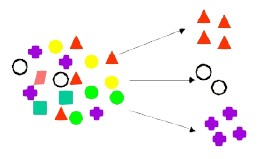
\includegraphics[height=50mm]{Figures/clustering.jpg}
\vspace{3.0cm}
% Title, author and degree
\vspace{1.0cm}
{\FontLb Efficient Evidence Accumulation Clustering for large datasets/big data} \\
%\vspace{0.2cm}
%{\FontMn Subtitle (optional)} \\
%\vspace{1.9cm}
\vspace{2.7cm}
{\FontMb Diogo Alexandre Oliveira Silva} \\
% {Alferes Aluno Engenheiro Electrotécnico 136787-A} \\
\vspace{2.0cm}
{\FontSn Thesis to obtain the Master of Science Degree in} \\
\vspace{0.3cm}
{\FontLb Electrical and Computer Engineering} \\
% {\FontLb Aeronautical Military Sciences in the speciality of Electrical Engineering} \\
\vspace{1.1cm}
{\FontSn Supervisors: Dra. Ana Luísa Nobre Fred \\ Dra. Helena Isabel Aidos Lopes} \\
\vspace{1.1cm}
{\FontMb Examination Committee} \\
\vspace{0.3cm}
{\FontSn %
\begin{tabular}{c}
Chairperson: Prof. Dr. João Fernando Cardoso Silva Sequeira \\
Supervisor: Dra. Ana Luísa Nobre Fred \\
% Co-supervisor: & Dra. Helena Aidos Lopes \\
Members of the Committee: Dr. Pedro Filipe Zeferino Tomás \\
 BGEN ENGEL José Manuel dos Santos Vicêncio \\% for FAP
 TCOR ENGEL Ana Paula da Silva Jorge% for FAP
\end{tabular} } \\
\vspace{1.5cm}
{\FontMb December 2015} \\
%
\end{center}

\cleardoublepage

 % file "Thesis_FrontCover.tex"

% ----------------------------------------------------------------------
% Dedication page (optional)
% ----------------------------------------------------------------------
% %%%%%%%%%%%%%%%%%%%%%%%%%%%%%%%%%%%%%%%%%%%%%%%%%%%%%%%%%%%%%%%%%%%%%%%%
%                                                                      %
%     File: Thesis_Dedication.tex                                      %
%     Tex Master: Thesis.tex                                           %
%                                                                      %
%     Author: Andre C. Marta                                           %
%     Last modified : 21 Jan 2011                                      %
%                                                                      %
%%%%%%%%%%%%%%%%%%%%%%%%%%%%%%%%%%%%%%%%%%%%%%%%%%%%%%%%%%%%%%%%%%%%%%%%

\null\vskip5cm%
\begin{flushright}
     Dedicated to someone special...
\end{flushright}
\vfill\newpage

\cleardoublepage

 % file "Thesis_Dedication.tex"

% ----------------------------------------------------------------------
%  Acknowledgments (optional)
% ----------------------------------------------------------------------
%%%%%%%%%%%%%%%%%%%%%%%%%%%%%%%%%%%%%%%%%%%%%%%%%%%%%%%%%%%%%%%%%%%%%%%%
%                                                                      %
%     File: Thesis_Acknowledgments.tex                                 %
%     Tex Master: Thesis.tex                                           %
%                                                                      %
%     Author: Andre C. Marta                                           %
%     Last modified : 21 Jan 2011                                      %
%                                                                      %
%%%%%%%%%%%%%%%%%%%%%%%%%%%%%%%%%%%%%%%%%%%%%%%%%%%%%%%%%%%%%%%%%%%%%%%%

\section*{\acknowledgments}

% Add entry in the table of contents as section
\addcontentsline{toc}{section}{\acknowledgments}

%Supervisors
It would come as a great oversight if I was not aware of the help and contribution I received for the completion of this undertaking.

I should start by expressing deep appreciation to my supervisors, Dr. Ana Fred and Dr. Helena Lopes.
The freedom I was allowed was crucial for keeping my motivation up for such a long period.
When that was lacking, their guidance and encouragement quickly put me back on track.

%Family & Friends
I leave my warmest regards to the family I built throughout my military and academic career, during these last years.
Your camaraderie has shaped where I stand and who I am today.
Your support throughout these long months was invaluable.

% Bella
To my loving girlfriend, who would always hear my boundless enthusiasm or disheartening frustrations, whichever was the case, and who followed me closest in the last months, I am deeply grateful.
You motivated me most of all, and that was no small task.

And to my parents, thank you for all your support and motivation during all these years.
You were always caring and encouraging and I am forever grateful for that.

Last, but not least, thank you to all my friends and family for understanding my absence during these challenging months.
\cleardoublepage

 % file "Thesis_Acknowledgements.tex"

% ----------------------------------------------------------------------
%  Abstract (both in English and Portuguese)
% ----------------------------------------------------------------------
%%%%%%%%%%%%%%%%%%%%%%%%%%%%%%%%%%%%%%%%%%%%%%%%%%%%%%%%%%%%%%%%%%%%%%%%
%                                                                      %
%     File: Thesis_Resumo.tex                                          %
%     Tex Master: Thesis.tex                                           %
%                                                                      %
%     Author: Andre C. Marta                                           %
%     Last modified : 21 Jan 2011                                      %
%                                                                      %
%%%%%%%%%%%%%%%%%%%%%%%%%%%%%%%%%%%%%%%%%%%%%%%%%%%%%%%%%%%%%%%%%%%%%%%%

\section*{Resumo}

% Add entry in the table of contents as section
\addcontentsline{toc}{section}{Resumo}

Avanços na tecnologia permitem a recolha e armazenamento de quantidades e variedades de dados sem precedente.
A maior parte destes dados são armazenados eletrónicamente e existe interesse em realizar análise automática dos mesmos.
As técnicas de \emph{clustering} estão entre as mais populares para essa tarefa porque não assumem nada sobre a estrutura dos dados \emph{a priori}.
Muitas técnicas existem, mas, típicamente, não têm um bom desempenho em todos os conjuntos de dados devido às especifidades de cada um.
Técnicas de \emph{ensemble clustering} tentam responder a esse desafio ao combinar outros algoritmos.
Esta dissertação foca-se numa em particular, o \emph{Evidence Accumulation Clustering} (EAC).
O EAC é uma algorithm robusto que tem demonstrado bons desempenhos na literatura numa variedade de conjuntos de dados.
No entanto, esta robustez vem com um maior custo computacional associado.
A sua aplicação não só é mais lenta como está restrita a conjuntos de dados pequenos.
Assim, o objetivo desta dissertação é escalar o EAC, possibilitando a sua a aplicação a conjuntos de dados grandes, com tecnologia disponivel numa típica estação de trabalho.
Com isto em mente, várias abordagens foram exploradas: acelerar processamento com outros algoritmos (\emph{quantum clustering}), através de processamento paralelo (com GPU), escalar com algoritmos de memória externa (disco rígido) e explorando a natureza esparsa do EAC.
Além disto, foi desenvolvido um método eficiente para construir uma matriz esparsa específico ao EAC.
A solução proposta é aplicável a conjuntos de dados grandes e é entre 6 a 200 vezes mais rápida que a original para conjuntos pequenos.

\vfill

\textbf{\Large Palavras-chave:} Métodos de agrupamento, EAC, K-Means, MST, GPGPU, CUDA, Matrizes esparsas, Single-Link

\cleardoublepage

 % file "Thesis_Resumo.tex"
%%%%%%%%%%%%%%%%%%%%%%%%%%%%%%%%%%%%%%%%%%%%%%%%%%%%%%%%%%%%%%%%%%%%%%%%
%                                                                      %
%     File: Thesis_Abstract.tex                                        %
%     Tex Master: Thesis.tex                                           %
%                                                                      %
%     Author: Andre C. Marta                                           %
%     Last modified : 21 Jan 2011                                      %
%                                                                      %
%%%%%%%%%%%%%%%%%%%%%%%%%%%%%%%%%%%%%%%%%%%%%%%%%%%%%%%%%%%%%%%%%%%%%%%%

\section*{Abstract}

% Add entry in the table of contents as section
\addcontentsline{toc}{section}{Abstract}

Advances in technology allow for the collection and storage of an unprecedent amount and variety of data.
Most of this data is stored electronically and there is an interest in automated analysis for generation of knowledge and new insights.
Since the structure of the data is unknown, clustering techniques become particularly interesting for knowledge discovery and data mining, as they make as few assumptions on the data as possible.
A vast body of work on these algorithms exist, yet, typically, no single algorithm is able to respond to the specificities of all data.
Ensemble clustering algorithm address this problem by combining other algorithms.
Evidence Accumulation Clustering (EAC) is a robust ensemble algorithm that has shown good results and is the focus of this dissertation.
However, this robustness comes with higher computational cost.
Its application is slower and restricted to smaller datasets.
Thus, the objective of this dissertation is to scale EAC, allowing its applicability to big datasets, with technology available at a typical workstation.
Accordingly, several approaches were explored: speed-up with other algorithms (\emph{quantum clustering}) or parallel computing (with GPU) and reducing space complexity by using external memory (hard drive) algorithms and exploiting the sparse nature of EAC.
A relevant contribution is a novel method to build a sparse matrix specialized in EAC.
Results show that the proposed solution is applicable to large datasets and presents speed-ups between 6 and 200 over the original implementation on different phases of EAC for small datasets.

\vfill

\textbf{\Large Key words:} Clustering methods, EAC, K-Means, MST, GPGPU, CUDA, Sparse matrices, Single-Link

\cleardoublepage

 % file "Thesis_Abstract.tex"

% ----------------------------------------------------------------------
%  Table of contents, list of tables, list of figures and nomenclature
% ----------------------------------------------------------------------

% Table of contents
%
\tableofcontents
\cleardoublepage 

% List of tables
%
% Generate list
\listoftables
% Add entry in the table of contents as section
\addcontentsline{toc}{section}{\listtablename}
\cleardoublepage 

% List of figures
%
% Generate list
\listoffigures
% Add entry in the table of contents as section
\addcontentsline{toc}{section}{\listfigurename}
\cleardoublepage 

% Nomenclature
%
% entries of nomenclature list
%%%%%%%%%%%%%%%%%%%%%%%%%%%%%%%%%%%%%%%%%%%%%%%%%%%%%%%%%%%%%%%%%%%%%%%%%
%                                                                      %
%     File: Thesis_Nomenclature.tex                                    %
%     Tex Master: Thesis.tex                                           %
%                                                                      %
%     Author: Andre C. Marta                                           %
%     Last modified : 21 Jan 2011                                      %
%                                                                      %
%%%%%%%%%%%%%%%%%%%%%%%%%%%%%%%%%%%%%%%%%%%%%%%%%%%%%%%%%%%%%%%%%%%%%%%%
%
% The definitions can be placed anywhere in the document body
% and their order is sorted by <symbol> automatically when
% calling makeindex in the makefile
%
% The \glossary command has the following syntax:
%
% \glossary{entry}
%
% The \nomenclature command has the following syntax:
%
% \nomenclature[<prefix>]{<symbol>}{<description>}
%
% where <prefix> is used for fine tuning the sort order,
% <symbol> is the symbol to be described, and <description> is
% the actual description.

% ----------------------------------------------------------------------
% Roman symbols [r]
\nomenclature[ru]{$\bf u$}{Velocity vector.}
\nomenclature[ru]{$u,v,w$}{Velocity Cartesian components.}
\nomenclature[rp]{$p$}{Pressure.}
\nomenclature[rC]{$C_D$}{Coefficient of drag.}
\nomenclature[rC]{$C_L$}{Coefficient of lift.}
\nomenclature[rC]{$C_M$}{Coefficient of moment.}

% ----------------------------------------------------------------------
% Greek symbols [g]
\nomenclature[g]{$\rho$}{Density.}
\nomenclature[g]{$\alpha$}{Angle of attack.}
\nomenclature[g]{$\beta$}{Angle of side-slip.}
\nomenclature[g]{$\mu$}{Molecular viscosity coefficient.}
\nomenclature[g]{$\kappa$}{Thermal conductivity coefficient.}

% ----------------------------------------------------------------------
% Subscripts [s]
\nomenclature[s]{$x,y,z$}{Cartesian components.}
\nomenclature[s]{$i,j,k$}{Computational indexes.}
\nomenclature[s]{$\infty$}{Free-stream condition.}
\nomenclature[s]{ref}{Reference condition.}
\nomenclature[s]{$n$}{Normal component.}

% ----------------------------------------------------------------------
% Supercripts [t]
\nomenclature[t]{T}{Transpose.}
\nomenclature[t]{*}{Adjoint.}

 % file "Thesis_Nomenclature.tex"
%
% Insert glossary/nomenclature section produced by MakeIndex
%\printnomenclature
% Add entry in the table of contents as section
%\addcontentsline{toc}{section}{\nomname}
%\cleardoublepage

% entries of glossary list
%%%%%%%%%%%%%%%%%%%%%%%%%%%%%%%%%%%%%%%%%%%%%%%%%%%%%%%%%%%%%%%%%%%%%%%%
%                                                                      %
%     File: Thesis_Glossary.tex                                        %
%     Tex Master: Thesis.tex                                           %
%                                                                      %
%     Author: Andre C. Marta                                           %
%     Last modified : 30 Oct 2012                                      %
%                                                                      %
%%%%%%%%%%%%%%%%%%%%%%%%%%%%%%%%%%%%%%%%%%%%%%%%%%%%%%%%%%%%%%%%%%%%%%%%
%
% The definitions can be placed anywhere in the document body
% and their order is sorted by <symbol> automatically when
% calling makeindex in the makefile
%
% The \glossary command has the following syntax:
%
% \glossary{entry}
%
% The \nomenclature command has the following syntax:
%
% \nomenclature[<prefix>]{<symbol>}{<description>}
%
% where <prefix> is used for fine tuning the sort order,
% <symbol> is the symbol to be described, and <description> is
% the actual description.

% ----------------------------------------------------------------------

% QUANTUM CLUSTERING
\glossary{name={\textbf{Qubit}},description={Quantum bit}}
\glossary{name={\textbf{QK-Means}},description={Quantum K-Means}}
\glossary{name={\textbf{QC}},description={Quantum clustering}}

\glossary{name={\textbf{PCA}},description={Principal Component Analysis}}
\glossary{name={\textbf{PC}},description={Principal Component}}

% EAC
\glossary{name={\textbf{EAC}},description={Evidence Accumulation Clustering}}
\glossary{name={\textbf{SL}},description={Single Link}}
\glossary{name={\textbf{HAC}},description={Hierarchical Agglomeration Clustering}}
\glossary{name={\textbf{MST}},description={Minimum Spanning Tree}}

% GPU
\glossary{name={\textbf{CPU}},description={Central Processing Unit}}
\glossary{name={\textbf{GPU}},description={Graphics Processing Unit}}
\glossary{name={\textbf{GPGPU}},description={General Purpose computing in Graphics Processing Units}}

\glossary{name={\textbf{API}},description={Application Programming Interface}}


\glossary{name={\textbf{FCM}},description={Fuzzy C-Means}}
\glossary{name={\textbf{SL-MST}},description={Single-Link based on Minimum Spanning Tree}}
\glossary{name={\textbf{WEAC}},description={Weighted Evidence Accumulation Clustering}} % file "Thesis_Glossary.tex"

% Insert glossary section produced by MakeIndex
\printglossary
% Add entry in the table of contents as section
\addcontentsline{toc}{section}{\glossaryname}
\cleardoublepage

% Set arabic numbering (1,2,...) after preface
%
\setcounter{page}{1}
\pagenumbering{arabic}

% ----------------------------------------------------------------------
%  Chapters
% ----------------------------------------------------------------------

%--------------------------------------------%
%--------------------------------------------%
%    INTROCUTION 
%--------------------------------------------%
%--------------------------------------------%

\section{Introduction}
%    CLUSTERING
%--------------------------------------------%
\subsection{Clustering}

% FRAME: WHAT IS CLUSTERING
\begin{frame}{What is clustering?}

``The goal of data clustering, also known as cluster analysis, is to discover the natural grouping(s) of a set of patterns, points, or objects.''
\footnote{A. K. Jain, “Data clustering: 50 years beyond K-means,” Pattern Recognition Letters, vol. 31}
%{\scriptsize A. K. Jain, “Data clustering: 50 years beyond K-means,” Pattern Recognition Letters, vol. 31}

\end{frame}
        
% FRAME: DIFFERENT CLUSTERING ALGORITHMS
% \begin{frame}{What is clustering?}

% \centering
% \includegraphics[width=0.8\columnwidth]{{{diff_algs_Fred2005}}}

% {\fontsize{5.5}{5.5} \selectfont Source: A. N. L. Fred and A. K. Jain, “Combining multiple clusterings using evidence accumulation,” IEEE Transactions on Pattern Analysis and Machine Intelligence, vol. 27}

% \end{frame}

\begin{frame}{What is clustering?}
\centering
\begin{tabular}{ccc}
  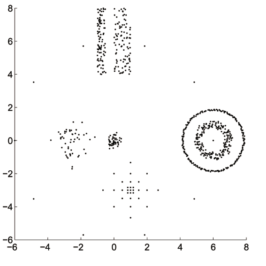
\includegraphics[width=0.3\textwidth]{diff_algs/raw} &   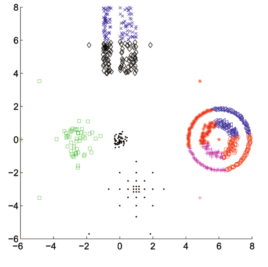
\includegraphics[width=0.3\textwidth]{diff_algs/b} & 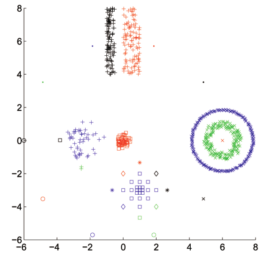
\includegraphics[width=0.3\textwidth]{diff_algs/c}  \\

  {\tiny (a)} & {\tiny (b)} & {\tiny (c)} \\

  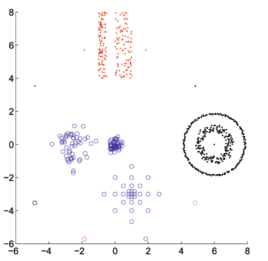
\includegraphics[width=0.3\textwidth]{diff_algs/d} &  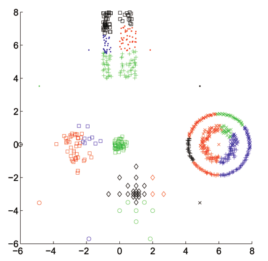
\includegraphics[width=0.3\textwidth]{diff_algs/e} &  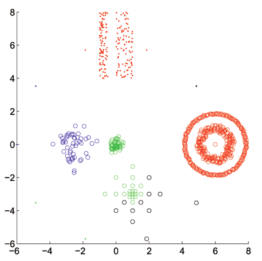
\includegraphics[width=0.3\textwidth]{diff_algs/f}\\

  {\tiny (d)} & {\tiny (e)} & {\tiny (f)}

\end{tabular}
{\fontsize{5.5}{5.5} \selectfont A. N. L. Fred and A. K. Jain, “Combining multiple clusterings using evidence accumulation”, IEEE Transactions on Pattern Analysis and Machine Intelligence, vol. 27}

\end{frame}


%--------------------------------------------%
%    EAC
%--------------------------------------------%
\subsection{EAC}
\begin{frame}{Evidence Accumulation Clustering}

\begin{itemize}
	\item State-of-the-art

	\item Robust

	\item Ensemble method

	% \item Robust state-of-the-art ensemble method

	% \item Three steps:
	% \begin{itemize}
	% 	\item \textbf{Production} of a clustering ensemble
	% 	\item \textbf{Combination} into a co-association matrix
	% 	\item \textbf{Recovery} of the natural clusters
	% \end{itemize}

	% \item More complex and computationally expensive

	% \item Harder to scale

\end{itemize}

\end{frame} 

\begin{frame}{EAC: Production}

\centering
\begin{tabular}{ccc}
  \includegraphics[width=0.3\textwidth]{EAC_plots/raw_data} &  & 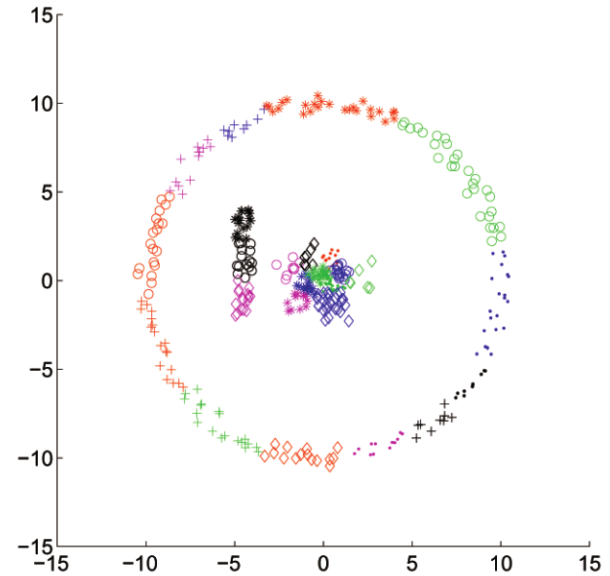
\includegraphics[width=0.3\textwidth]{EAC_plots/kmeans1} \\
 
   {\tiny (a)} & & {\tiny (b)} \\

  & &  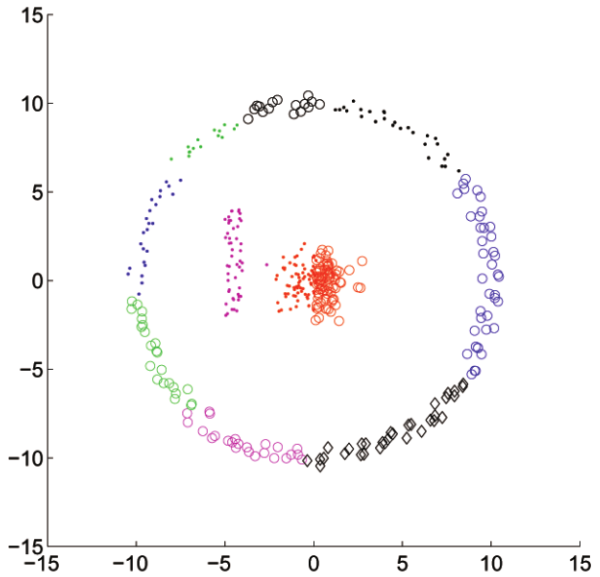
\includegraphics[width=0.3\textwidth]{EAC_plots/kmeans2} \\

  & & {\tiny (c)} \\
\end{tabular}

% {\fontsize{5.5}{5.5} \selectfont Source: A. N. L. Fred and A. K. Jain, “Combining multiple clusterings using evidence accumulation,” IEEE Transactions on Pattern Analysis and Machine Intelligence, vol. 27}

\end{frame}




\begin{frame}{EAC: Combination}

\centering
\begin{tabular}{ccc}
  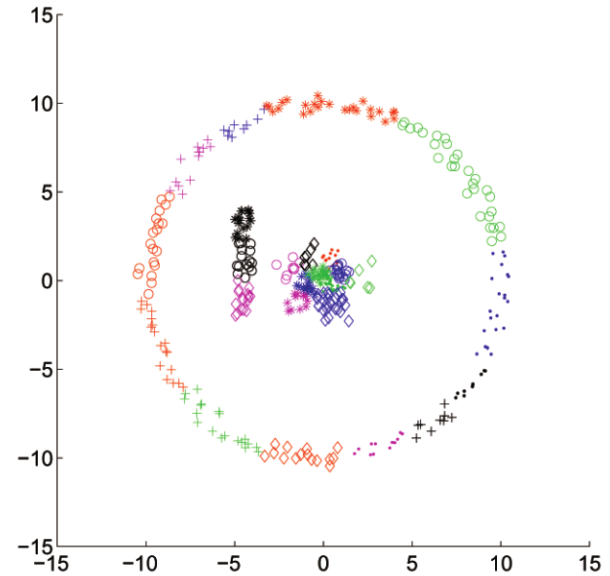
\includegraphics[width=0.3\textwidth]{EAC_plots/kmeans1} &   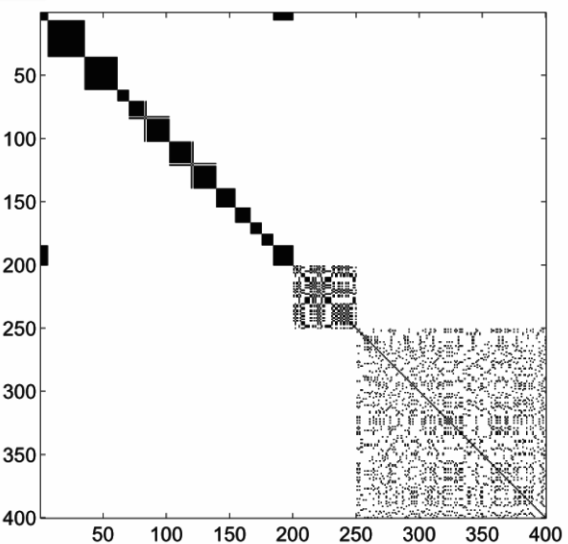
\includegraphics[width=0.3\textwidth]{EAC_plots/coassoc1} & 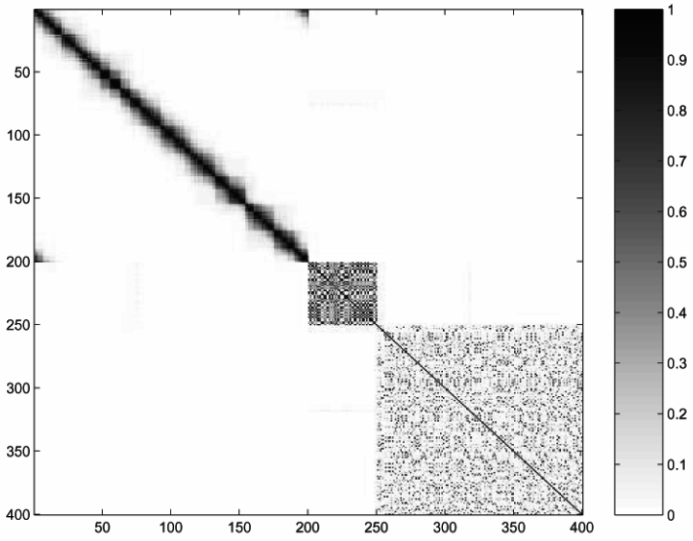
\includegraphics[width=0.3\textwidth]{EAC_plots/coassocEAC}  \\

  {\tiny (a)} & {\tiny (c)} & {\tiny (e)} \\

  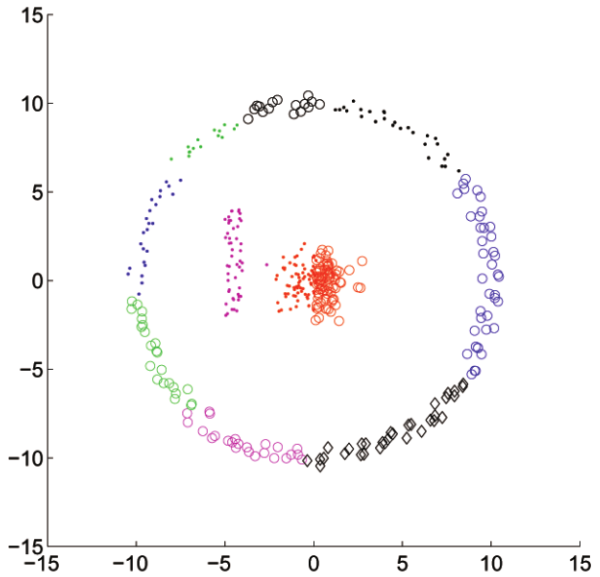
\includegraphics[width=0.3\textwidth]{EAC_plots/kmeans2} &  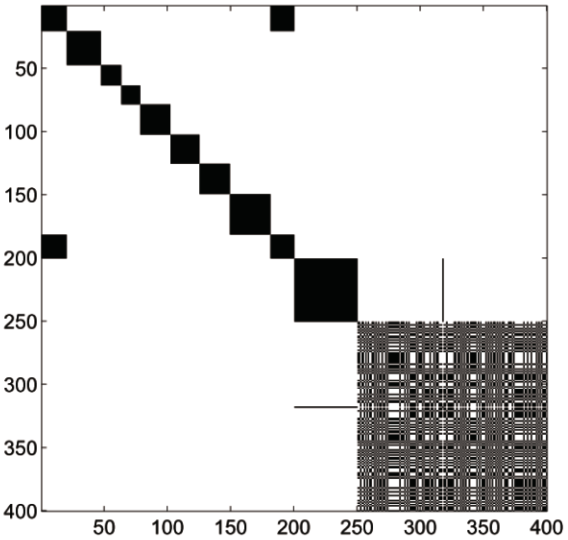
\includegraphics[width=0.3\textwidth]{EAC_plots/coassoc2} & \\

  {\tiny (b)} & {\tiny (d)} &

\end{tabular}

% {\fontsize{5.5}{5.5} \selectfont Source: A. N. L. Fred and A. K. Jain, “Combining multiple clusterings using evidence accumulation,” IEEE Transactions on Pattern Analysis and Machine Intelligence, vol. 27}

\end{frame}

\begin{frame}{EAC: Recovery}

\centering
\begin{tabular}{cc}
  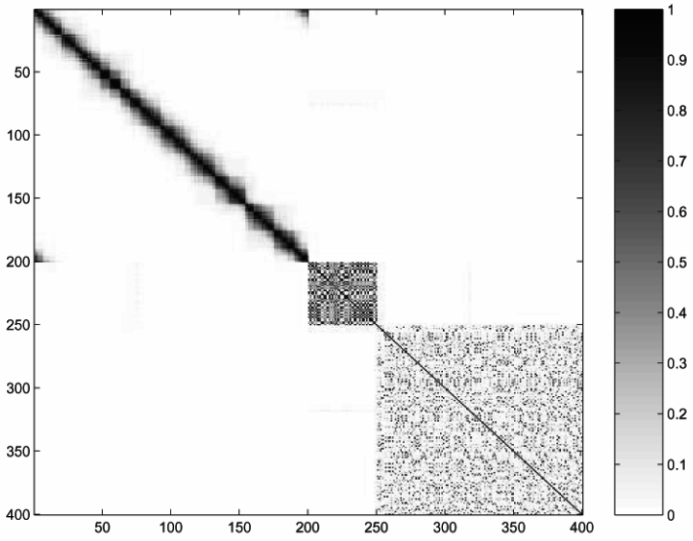
\includegraphics[width=0.3\textwidth]{EAC_plots/coassocEAC} &   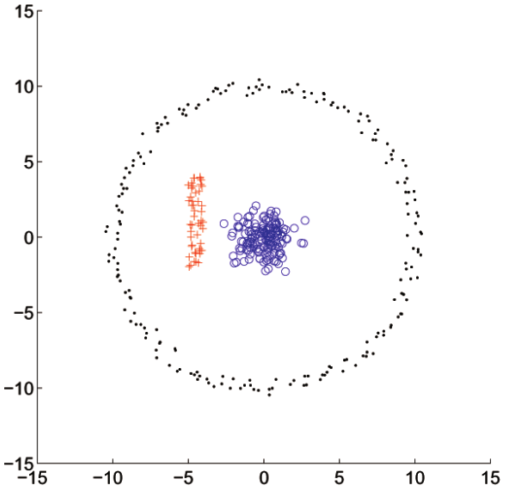
\includegraphics[width=0.3\textwidth]{EAC_plots/eac}  \\

  {\tiny (a)} & {\tiny (b)}
\end{tabular}


% {\fontsize{5.5}{5.5} \selectfont Source: A. N. L. Fred and A. K. Jain, “Combining multiple clusterings using evidence accumulation,” IEEE Transactions on Pattern Analysis and Machine Intelligence, vol. 27}

\end{frame}

\subsection{Goals}

\begin{frame}{Goals}
\begin{itemize}
% \item Study the integration of quantum inspired methods in EAC.
% \item Study the integration of the GPGPU paradigm in EAC.
\item Devise strategies to reduce computation and memory complexities of EAC.
\item Validation of Big Data EAC on real data.
\item Application of Evidence Accumulation Clustering to Big Data.
%\item Application of EAC to real-world large datasets.
\end{itemize}
\end{frame}    	 % file "Thesis_Introduction.tex"
%!TEX root = Thesis.tex

\chapter{Clustering: basic concepts, definitions and algorithms}
\label{chapter:clustering}

%this is mostly taken from Jain's 50 years beyond K-Means
Hundreds of methods for data analysis exist.
Many of these methods fall into the realm of machine learning, which is usually divided into 2 major groups: \textit{supervised} and \textit{unsupervised} learning.
% TODO: add some reference for the 2 major groups; optional: explain what learning is
Supervised learning deals with labeled data, i.e. data for which the ground truth is known, and tries to solve the problem of classification.
Examples of supervised learning algorithms are Neural Networks, Decision Trees, Linear Regression and Support Vector Machines. %TODO add refs
 %TODO: add ref for solving classification
Unsupervised learning deals with unlabeled data for which no extra information is known.
% An example of algorithms within this paradigm is clustering algorithms, which are the focus of this chapter.
Clustering methods are an example of unsupervised methods and are the focus of this chapter.
%Clustering algorithms an are example of unsupervised algorithms. % TODO: add refs

This chapter will serve as an introduction to clustering.
It starts by defining the problem of clustering in section \ref{sec:clustering}, goes on to provide useful definitions and notation in section \ref{sec:definitions and notation} and briefly addresses different properties of clustering algorithms in section \ref{sec:clustering properties}.
Two very well known algorithms are presented: K-Means in section \ref{sec:kmeans} and Single-Link in section \ref{sec:sl}.
Evidence Accumulation Clustering is a state of the art ensemble clustering algorithm and the focus of this dissertation.
Section \ref{sec:ensemble} will explain briefly the concept of ensemble clustering followed by an overview and application examples of the EAC algorithm in section \ref{sec:eac}.

\section{The problem of clustering}
\label{sec:clustering}

% have to say that I'm using a vectorial representation of the data (data as vector of features) without loss of generality. I have to specify that I'm dealing with a partitioning clustering but other kinds exist. In this context (of vectorial data and partitional algorithms) K-Means is one of the most known algorithms. It is simple and fast and, although it only yields good results in a specific set of cases, it is often used as a starting point for more robust algorithms, e.g. EAC. 

Cluster analysis methods are unsupervised and the backbone of the present work.
The goal of data clustering, as defined by \cite{Jain2010}, is the discovery of the \textit{natural grouping(s)} of a set of patterns, points or objects.
In other words, the goal of data clustering is to discover structure on data.
The methodology used is to group patterns (usually represented as a vector of measurements or a point in space \cite{Jain1999}) based on some similarity, such that patterns belonging to the same cluster are typically more similar to each other than to patterns of other clusters.
Clustering is a strictly data-driven method, in contrast with classification techniques which have a training set with the desired labels for a limited collection of patterns.
Because there is very little information, as few assumptions as possible should be made about the structure of the data (e.g. number of clusters).
Also, because clustering typically makes as few assumptions on the data as possible, it is appropriate to use it on exploratory data analysis.
The process of clustering data has three main aspects \cite{Jain1999}:

\begin{itemize}
    \item \textbf{Pattern representation} refers to the choice of representation of the input data in terms of size, scale and type of features.
    The input patterns may be fed directly to the algorithms or undergo \emph{feature selection} and/or \emph{feature extraction}.
    The former is simply the selection of which features should be used.
    The latter deals with the transformation of the original feature space such that the resulting space will produce more accurate and insightful clusterings, e.g. by applying Principal Component Analysis.
    % It should be noted that

    \item \textbf{Pattern similarity} refers to the definition of a measure for computing the similarity between two patterns.
    \item \textbf{Grouping} refers to the algorithm that will perform the actual clustering on the dataset with the defined pattern representation, using the appropriate similarity measure.
\end{itemize}

%TODO iris dataset reference
As an example, Figure \ref{fig:intro raw} shows the plot of the Iris dataset \cite{anderson1936species,fisher1936use}, a small well-known Machine Learning dataset.
This dataset has 4 features, of which only 2 are represented, and 3 classes, of which 2 are overlapping.
A class is overlapping another if they share part of the feature space, i.e. there is a region in the feature space whose patterns might belong to either class.
Figure \ref{fig:intro natural} presents the desired clustering for this dataset.

% Part of this went to the K-Means section
% The number of clusters was purposefully set to an "incorrect" number to demonstrate that the number of cluster of a dataset is not trivial to discover, even in such a simple example.
% In this synthetic dataset, the number of clusters is not clear due to the two superimposed Gaussians.
% The number of clusters is a common initialization parameter for clustering methods.
% When no prior information about the dataset is given, the number of clusters can be hard to discover.

\begin{figure}[!ht]
    \centering
    \begin{subfigure}[b]{0.45\textwidth}
        \centering
        \includegraphics[width=\textwidth]{clustering/raw_data}
        \caption{Input data, unlabeled.}
        \label{fig:intro raw}
    \end{subfigure}
    %\hfill
    \begin{subfigure}[b]{0.45\textwidth}
        \centering
        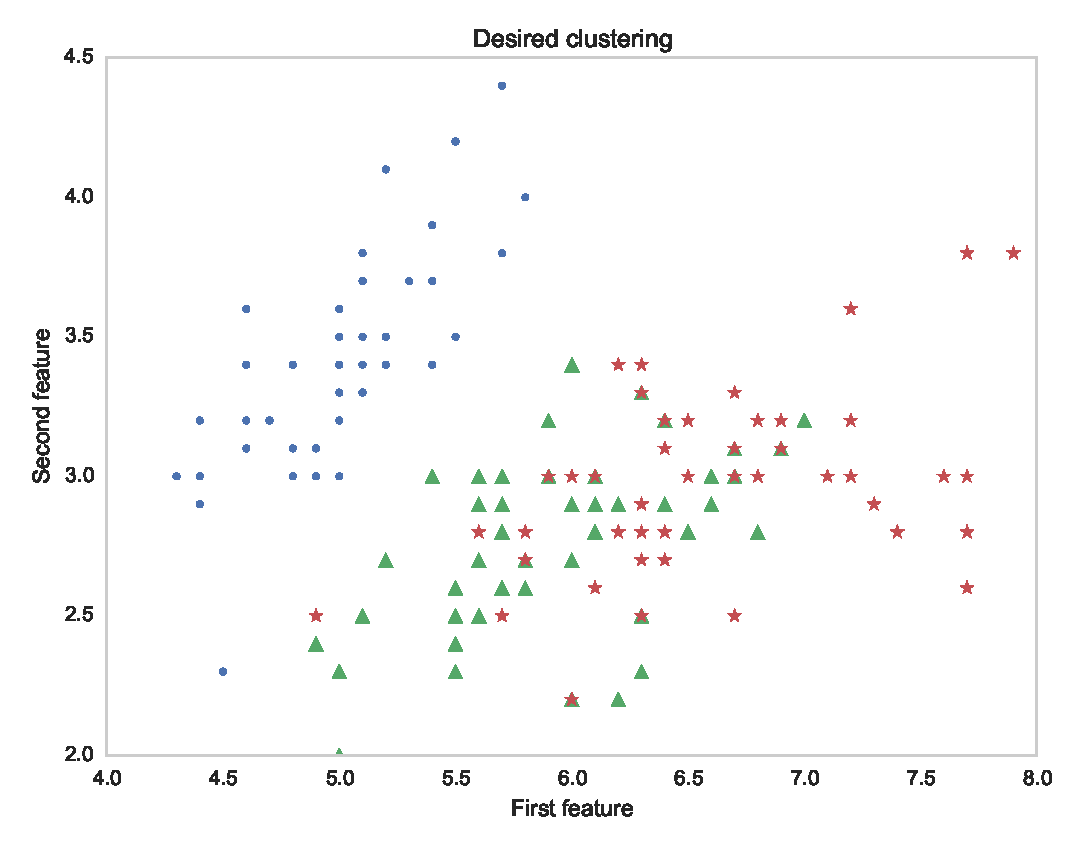
\includegraphics[width=\textwidth]{clustering/desired}
        \caption{Desired labels.}
        \label{fig:intro natural}
    \end{subfigure}

    \caption{First and second features of the Iris dataset. Fig. \ref{fig:intro raw} shows the scatter plot of the raw input data, i.e. how the algorithms "see" the data. Fig. \ref{fig:intro natural} shows the desired labels for each point, where each color and symbol are coded to a class.}
    \label{fig:clustering plots}
\end{figure}


\section{Definitions and Notation}
\label{sec:definitions and notation}

This section will introduce relevant definitions and notation within the clustering context that will be used throughout the rest of this document and were largely adopted from \cite{Jain1999}.

% TODO: review this part of the vector notation, it is fishy right now
%pattern, features
A \emph{pattern} $\mathbf{x}$ is a single data item and, without loss of generality, can be represented as a vector of $d$ \emph{features} $x_i$ that characterize that data item, $\mathbf{x} = (x_1, \ldots, x_d)$, where $d$ is referred to as the dimensionality of the pattern.
%pattern set
A \emph{pattern set} (or dataset) $\mathcal{X}$ is then the collection of all $n$ patterns $\mathcal{X} = \{ \mathbf{x}_1, \ldots, \mathbf{x}_n \}$.
The number of features is usually the same for all patterns in a given pattern set.

%classes
In cluster analysis, the desired clustering, typically, is one that reflects the natural structure of the data, i.e. the original ground truth labeling.
In other words, one wants to group the patterns that came from the same state of nature when they were generated, the same \emph{class}.
A class, then, can be viewed as a source of patterns and the effort of the clustering algorithm is to group patterns from the same source.
Throughout this work, these classes will also be referred to as the "natural" or "true" clusterings.
%labels
\emph{Hard} clustering (or partitional) techniques assign a class label $l_i$ to each pattern $\mathbf{x}_i$.
The whole set of labels corresponding to a pattern set $\mathcal{X}$ is given by $\mathcal{L} = \{ l_1, \ldots, l_n \}$, where $l_i$ is the label of pattern $\mathbf{x}_i$.
%partition
% Throughout this document, the whole set of labels may also be referred to as a partition.
Closely related to the whole set of labels is the concept of a \emph{partition}, which completely describes a clustering.
A partition $P$ is a collection of $k$ \emph{clusters}.
A cluster $C$ is a subset of $nc$ patterns $\mathbf{x}_i$ taken from the pattern set, where the patterns belonging to one subset do not belong to any other in the same partition.
A clustering \emph{ensemble} $\mathbb{P}$ is a set of $N$ partitions $P^j$ of a given pattern set, each composed of a set of $k_j$ clusters $C^j_i$, where $j=1, \ldots, N$, $i=1, \ldots, k_j$.
Each cluster is composed of a set of $nc^j_i$ patterns that does not intercept any other cluster of the same partition.
The relationship between the above concepts is condensed in the following expressions:

\begin{align*}
    ensemble \qquad & \mathbb{P} = \left \{   P^1, P^2, \ldots P^N   \right \}  \\
    partition \qquad & P^j = \left \{   C^j_1, C^j_2, \ldots C^{j}_{k_j}   \right \}  \\
    cluster \qquad & C^j_i = \left \{   x_1, x_2, \ldots x_{nc^j_i}   \right \}
\end{align*}



%TODO do this part better
%similarity
% Em relação aos conceitos: Proximidade não tem que ser métrica e pode ser semelhança ou dissemelhança. Pode sempre converter-se semelhança em dissemelhança e vice-versa, no entanto o mesmo já não acontece quando se convertem métricas. Uma distância é uma dissemelhança que é uma métrica (obedece às várias propriedades de métrica: simetria; d(x,x)=0 e desigualdade triangular). Quando se faz a conversão de uma distância para uma semelhança pode deixar de ser métrica. Mas isso só é mesmo importante quando se está a usar explicita ou implicitamente no processamento (por exemplo procura de vizinhos mais próximos, etc) a característica de desigualdade triangular. Em geral a propriedade de simetria é suficiente (e que d(x,x)=0 e sim(x,x)>sim(x,y)).

Typically, a clustering algorithm will use a \emph{proximity} measure for determining how alike are two patterns.
A proximity measure can either be a \emph{similarity} or a \emph{dissimilarity} measure, as one can easily be converted to the other.
The main difference is that the former increases in value as patterns are more alike, while the latter decreases in value.
A \emph{distance} is a dissimilarity function \emph{d} which yields non-negative real values and is also a \emph{metric}, which means it obeys the following three properties:



\begin{align*} 
    identity \qquad & d(\mathbf{x}_i, \mathbf{x}_i) = 0  \\
    symmetry \qquad & d(\mathbf{x}_i, \mathbf{x}_j) = d(\mathbf{x}_j, \mathbf{x}_i), i \neq j \\ 
    triangle \; inequality \qquad & d(\mathbf{x}_i, \mathbf{x}_j) + d(\mathbf{x}_j, \mathbf{x}_z)  \ge d(\mathbf{x}_x, \mathbf{x}_z)
\end{align*}



% \begin{align}
%     identity \qquad & d(\mathbf{x}_i, \mathbf{x}_i) = 0  \label{eq:identity} \\
%     symmetry \qquad & d(\mathbf{x}_i, \mathbf{x}_j) = d(\mathbf{x}_j, \mathbf{x}_i), i \neq j   \label{eq:symmetry} \\
%     triangle \; inequality \qquad & d(\mathbf{x}_i, \mathbf{x}_j) + d(\mathbf{x}_j, \mathbf{x}_z) \ge d(\mathbf{x}_x, \mathbf{x}_z) \label{eq:triangle inequality}
% \end{align}

where $\mathbf{x}_i$, $\mathbf{x}_j$ and $\mathbf{x}_z$ are 3 distinct patterns belonging to the pattern set $\mathcal{X}$.
Examples of proximity measures include the Euclidean distance, the Pearson’s correlation coefficient and Mutual Shared Neighbors \cite{jarvis1973clustering}.
It should be noted that different proximity measures may be more appropriate in different contexts, such as document, biological or time-series clustering.
Furthermore, data can come in different types such as numerical (discrete or continuous) or categorical (binary or multinomial) attributes.
The researcher should take these factors into account as different proximity measures are more appropriate for some type or even heterogeneous type data. 

An introduction of clustering would be incomplete without a discussion on how good is a partition after clustering.
Several \emph{validity measures} exist and they can placed in two main categories \cite{Aggarwal2014}.
\emph{External} measures use \emph{a priori} information about the data to evaluate the clustering against some external structure.
An application of an external measure could be to test how accurate a clustering algorithm is for a particular dataset by matching the output partition against the ground truth.
The \emph{Consistency Index} \cite{Fred2001} and the H-index \cite{Meila2003} are examples of such measures that will be used in this work. %a measure of accuracy based on the problem of minimum weighted bipartite graphs matching \cite{lange2004stability}, which throughout the remainder of the present work will be refered to as \emph{H-index}.
%Both these methods are based matching clusters by the number of co-occurrences they have, i.e.
Both of them are based on giving a score to each pair of clusters from two different partitions and then choosing the pairs that produce the best overall score.
\emph{Internal} measures, on the other hand, determine the quality of the clustering without the use of external information about the data.
The Davies-Bouldin index \cite{davies1979cluster} is such a measure.
This index outputs a high score to partitions with high inter-cluster distance and low intra-cluster distance, and vice versa.




\section{Characteristics of clustering techniques}
\label{sec:clustering properties}

Clustering algorithms may be categorized and described according to different properties.
For the sake of completeness, a brief discussion of some of their properties will be layed out in this section.

% hierarchical and partitional
%\emph{Partitional} and \emph{hierarchical} algorithms are the two most studied kinds of algorithms \cite{Aggarwal2014}.
It is common to organize cluster algorithms into two distinct types: \emph{partitional} and \emph{hierarchical}.
A partitional algorithm, such as K-Means, is a hard clustering algorithm that will output a partiton where each pattern belongs exclusively to one cluster.
A hierarchical algorithm produces a tree-based data structure called \emph{dendrogram}.
A dendrogram contains different partitions at different levels of the tree which means that the user can easily change the desired number of clusters by simply traversing the different levels.
This is an advantage over a partitional algorithm since a user can analyze different partitions with different numbers of clusters without having to rerun the algorithm.
% agglomerative vs divisive
Hierarchical algorithms can be further split into two approaches: bottom-up (or \emph{agglomerative}) and top-down (or \emph{divisive}).
% agglomerative
The former starts with all patterns as distinct clusters and will group them together according to some dissimilarity measure, building the dendrogram from the ground up; examples of algorithms that take this approach are Single-Link and Average-Link.
%divisive
The latter will start will all patterns in the same cluster and continuously split it until all patterns are separated, building the dendrogram from the top level to the bottom; this approach is taken by the Principal Directon Divisive Partitioning \cite{Boley1998} and Bisecting K-Means \cite{Steinbach2000} algorithms.


% monothetic vs polithetic
Another characteristic relates to how algorithms use the features for computing similarities.
If all features are used simultaneously the algorithm is called \emph{polithetic}, e.g. K-Means.
Otherwise, if the features are used sequentially, it is called \emph{monothetic}, e.g. \cite{Chavent1998}.

% fuzzy clustering
Contrasting with \emph{hard} clustering algorithms, are the \emph{fuzzy} algorithms.
A fuzzy algorithm will attribute to each pattern a degree of membership to each cluster.
A partition can still be extracted from this output by choosing, for each pattern, the cluster with higher degree of membership.
An example of a fuzzy algorithm is the Fuzzy C-Means \cite{Bezdek1984}.

% stochastic vs deterministic
Another characteristic is an algorithm's stochasticity.
A \emph{stochastic} algorithm uses a probabilistic process at some point in the algorithm, possibly yielding different results in each run.
As an example, the K-Means algorithm typically picks the initialization centroids randomly.
A \emph{deterministic} algorithm, on the other hand, will always produce the same result for a given input, e.g. Single-Link.

Finally, the last characteristic discussed is how an algorithm processes the input data.
An algorithm is said to be \emph{incremental} if it processes the input incrementally, i.e. taking part of the data, processing it and then doing the same for the remaining parts, e.g. PEGASUS \cite{Kang2011}.
A \emph{non-incremental} algorithm, on the other hand, will process the whole input in each run, e.g. K-Means.
This discussion is specially relevant when considering large datasets that may not fit in memory or whose processing would take too long for a single run and is therefore done in parallel.



% % examples of cluster analysis
% Cluster analysis is a relevant technique across several domains (\cite{Aggarwal2014}):

% \begin{itemize}
% 	\item grouping users with similar behaviour or preferences in \textbf{customer segmentation};
% 	\item image segmentation in the field of \textbf{image processing};
% 	\item clustering gene expression data, among other application, in the domain of \textbf{biological data analysis};
% 	\item generation of hierarchical structure for easy access and retrieval of \textbf{information systems}; % not referenced in book
% \end{itemize}

% Clustering is used in a wide variety of fields to solve numerous problems, e.g.:
% %TODO provide references to all of this
% % see https://sites.google.com/site/dataclusteringalgorithms/clustering-algorithm-applications
% % has applications with articles
% \begin{itemize}
% \item image segmentation in the field of image processing;
% \item generation of hierarchical structure for easy access and retrieval of information systems;
% \item recommender systems by grouping users by their behaviour and/or preferences;
% \item clustering customers for targeted marketing in 
% \item clustering gene expression data in biology;
% \item grouping of 
% \end{itemize}



\section{K-Means}
\label{sec:kmeans}

One of the most famous non-optimal solutions for the problem of partitional clustering is the K-Means algorithm \cite{kmeansoriginal}.
The K-Means algorithm uses $K$ \emph{centroid} representatives, $c_k$, for $K$ clusters.
Patterns are assigned to a cluster such that the squared error (or, more accurately, squared dissimilarity measure) between the cluster representatives and the patterns is minimized.
In essence, K-Means is a solution (although not necessarily an optimal one) to an optimization problem having the Sum of Squared Errors as its objective function, which is known to be a computationally NP hard problem \cite{Jain2010}.
It can be mathematically demonstrated that the optimal representatives for the clusters are the means of the patterns of each cluster \cite{Aggarwal2014}.
K-Means, then, minimizes the following expression, where the proximity measure used is the Euclidean distance:

\begin{align}
    \sum^K_{k=1} \sum_{\mathbf{x}_i \in C_k} \| \mathbf{x}_i - c_k  \| ^2  \label{eq:sse}
\end{align}

K-Means needs two initialization parameters: the number of clusters and the centroid initializations.
It starts by assigning each pattern to its closer cluster based on the cluster's centroid.
This is called the \textbf{labeling} step since one usually uses cluster labels for this assignment.
The centroids are then recomputed based on this assignment, in the \textbf{update} step.
The new centroids are the mean of all the patterns belonging to the clusters, hence the name of the algorithm.
% convergence
These two steps are executed iteratively until a stopping condition is met, usually the number of iterations, a convergence criteria or both.
The initial centroids are usually chosen randomly, but other schemes exist to improve the overall accuracy of the algorithm, e.g. K-Means++ \cite{Arthur2007}.
There are also methods to automatically choose the number of clusters \cite{Aggarwal2014}.

% similarity measures
The proximity measure used is typically the Euclidean distance.
This tends to produce hyperspherical clusters \cite{Jain1999}.
Still, according to \cite{Jain2010}, other measures have been used such as the L1 norm, Mahalanobis distance, as well as the cosine similarity \cite{Aggarwal2014}.
The choice of similarity measure must be made carefully as it may not guarantee that the algorithm will converge.

% empty clusters
A detail of implementation is what to do with clusters that have no patterns assigned to them.
One approach to this situation is to drop the empty clusters in further iterations.
However, allowing the existence of empty clusters or dropping empty clusters is undesirable since the number of clusters is an input parameter and it is expected that the output contains the specified number of clusters.
Other approaches exist dealing with this problem, such as equaling the centroid of an empty cluster to the pattern furthest away from its assigned centroid or reusing the old centroids as in \cite{Pakhira2009}.

% kmeans as a step for other algorithms
K-Means is a simple algorithm with reduced complexity $O(ntk)$, where $n$ is the number of patterns in the pattern set, $k$ is the number of clusters and $t$ is the number of iterations that it executes.
Accordingly, K-Means is often used as a foundational step of more complex and robust algorithms, such as the EAC algorithm.

% After the first iteration, the first step is executed with the new centroids.
% The end result of the algorithm is the labels produced in the first step of the last iteration.

% The sequential K-Means algorithm is composed by two main stages \cite{Jain2010}:

% \begin{enumerate}
%     \item \textbf{labeling stage} for the assigning labels to each pattern of the dataset, e.g. the label of the $i-th$ pattern is $0$ if the minimum distance is to the $0-th$ centroid;
%     \item \textbf{update stage} for the computation of the new centroids based on the labels assignment, i.e. the new centroids will be the mean of all the patterns assigned to it.
% \end{enumerate}

%example
As an example, the evolution and output of the K-means algorithm to the data presented in Fig. \ref{fig:clustering plots} is represented in Fig. \ref{fig:intro kmeans}.
The algorithm was executed with 3 random centroids.

\begin{figure}[hbtp]
    \centering
    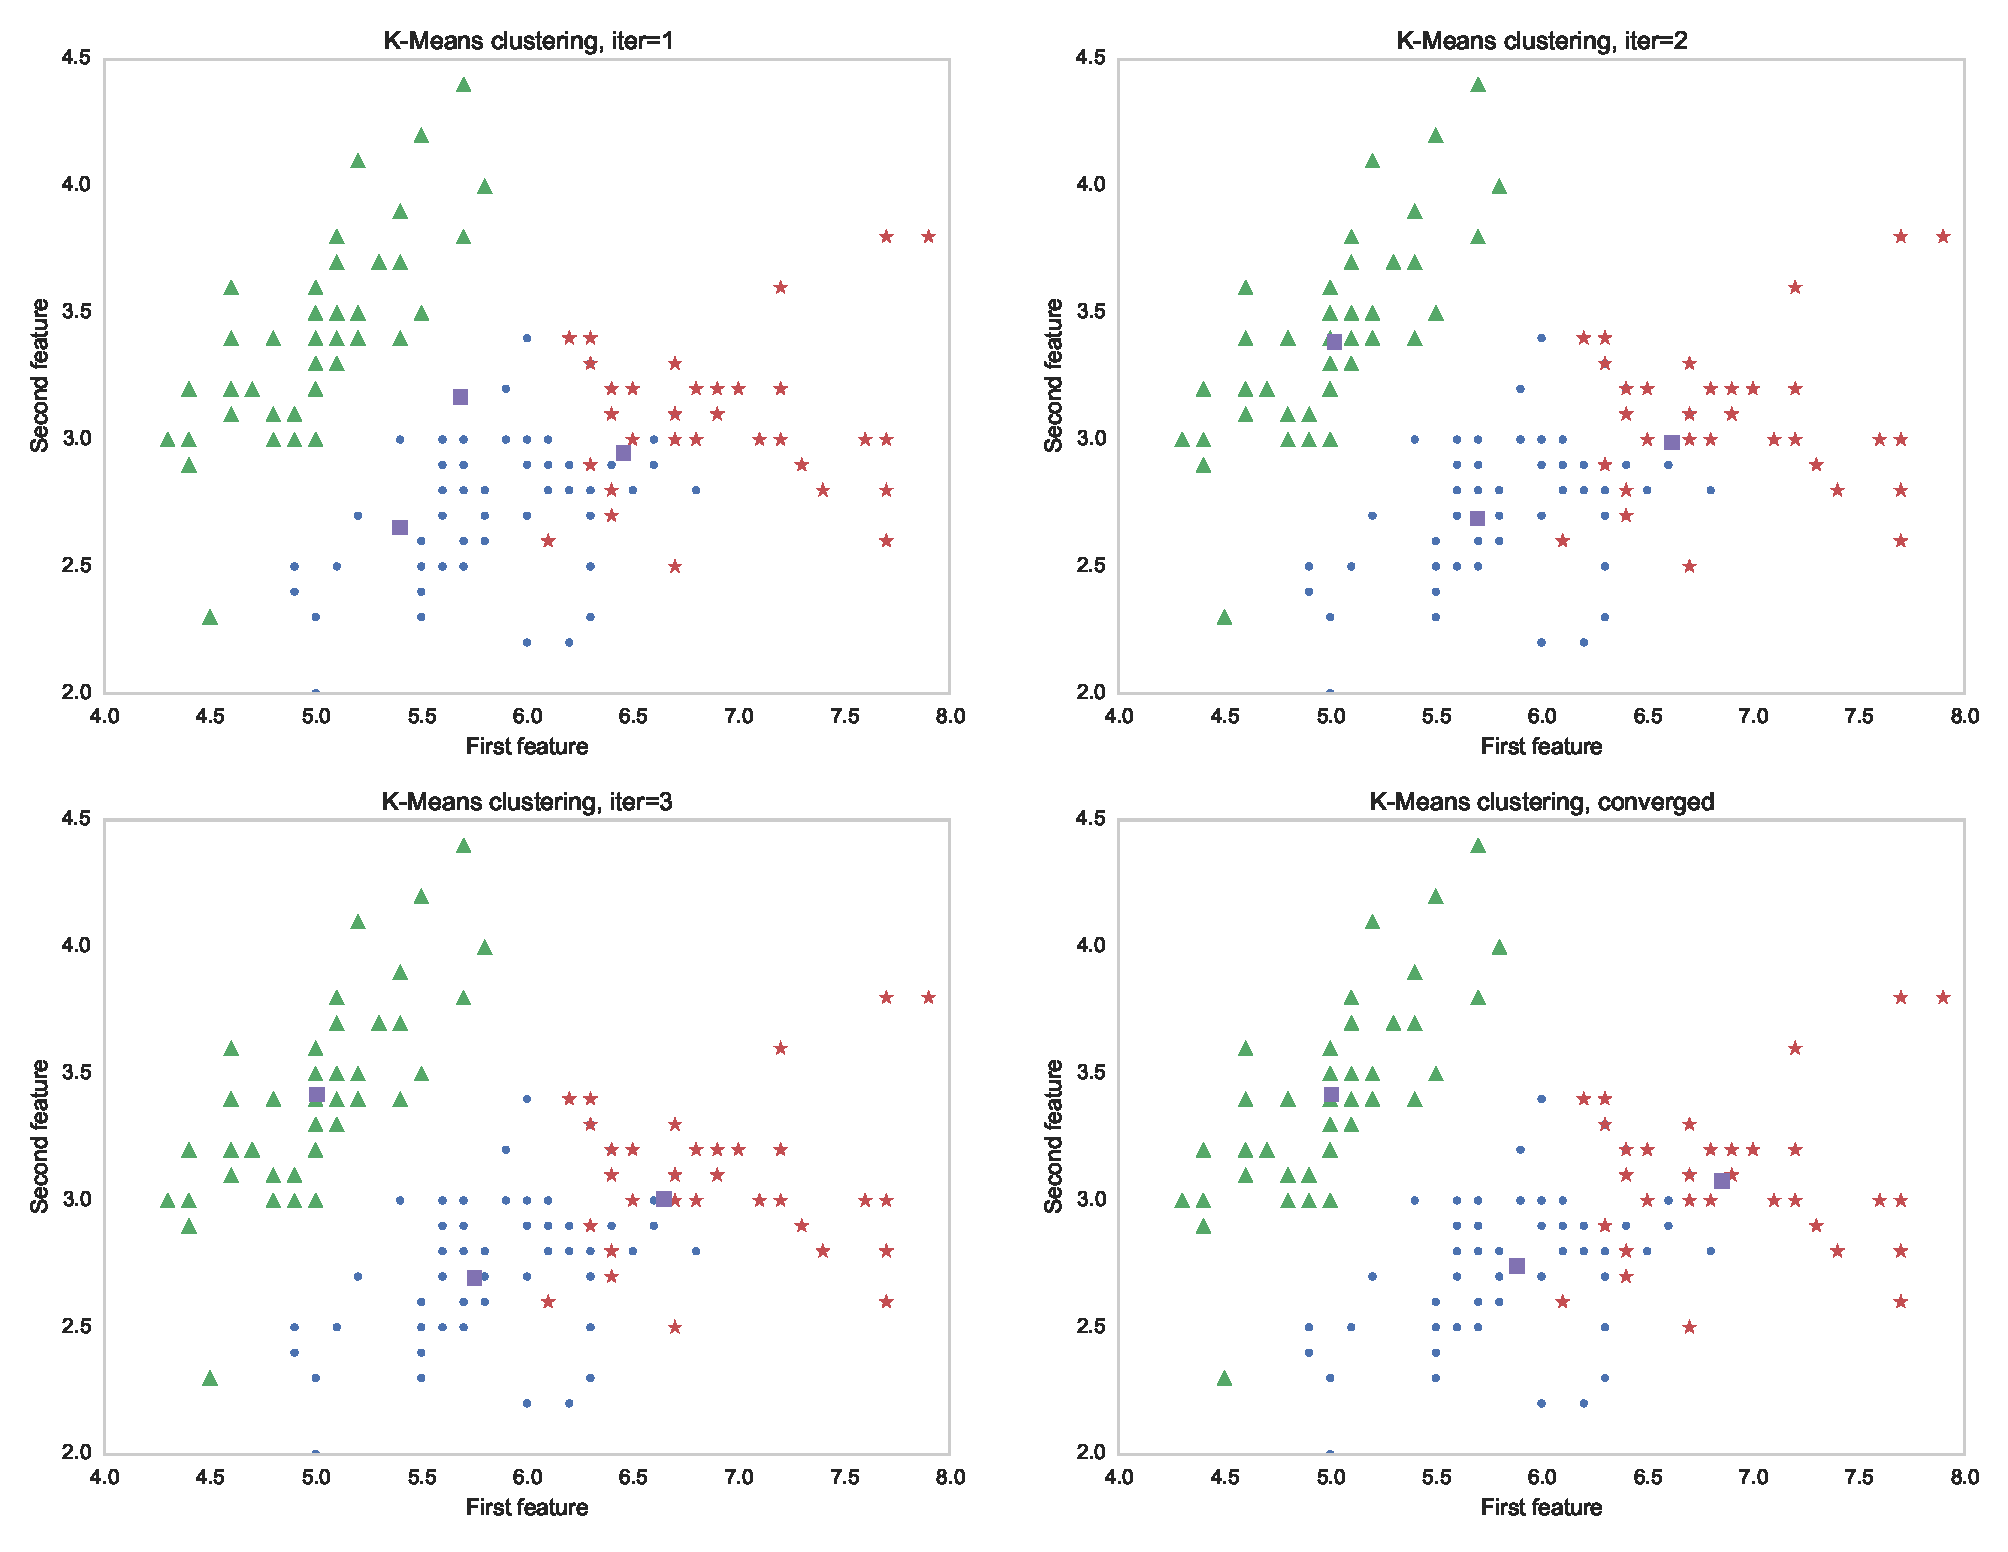
\includegraphics[width=\textwidth]{clustering/kmeans_progress}
    \caption{The output labels of the K-Means algorithm with the number of clusters (input parameter) set to 3. The different plots show the centroids (squares) evolution on each iteration. Between iteration 3 and the converged state 2 more iterations were executed.}
    \label{fig:intro kmeans}
\end{figure}

Even with the correct number of clusters, the clustering results do not match $100\%$ the natural clusters.
The accuracy relative to the natural clusters of Fig. \ref{fig:intro natural} is $88\%$ as measured by the Consistency Index (CI) \cite{Fred2001}.
In this example, the problem is the two overlapping clusters.
It is hard for an algorithm to discriminate between two clusters when they have similar patterns.
When no prior information about the dataset is given, the number of clusters can be hard to discover.
This is why, when available, a domain expert may provide valuable insight on tuning the initialization parameters.
% Others approaches, not addressed in this thesis, include the area of constrained clustering.

\section{Single-Link}
\label{sec:sl}

Single-Link \cite{sneath1962numerical} is one of the most popular hierarchical agglomerative clustering (HAC) algorithms.
HAC algorithms operate over a pair-wise dissimilarity matrix and output a dendrogram (e.g. Fig \ref{fig:sl dendrogram}).
The main steps of an agglomerative hierarchical clustering algorithm are the following \cite{Jain1999}:
\begin{enumerate}
    \item Create a pair-wise dissimilarity matrix of all patterns, where each pattern is a distinct cluster singleton;

    \item Find the closest clusters, merge them and update the matrix to reflect this change. The rows and columns of the two merged clusters are deleted and a new row and column are created to store the new cluster.% whose dissimilarities to other clusters will be the minimum of either the merging clusters.

    \item Stop if all patterns belong to a single cluster, otherwise continue to step 2.
\end{enumerate}

The algorithm stops when $n-1$ merges have been performed, which is when all patterns have been connected in the same cluster.
Just like in the K-Means algorithm, different similarity measures can be used between pairs of objects.

%different linkages
The proximity measure between clusters in the second step distinguishes between the different HAC linkage algorithms, such as Single-Link , Average-Link, Complete-Link, among others.
In Single-Link (SL), the proximity between any two clusters is the the dissimilarity between their closest patterns.
On the other hand, in Complete-Link, it is the proximity between their most distant patterns and, in Average-Link, is the proximity between the average point of each cluster.
In SL, because the algorithm connects first clusters that are more similar, it naturally gives more importance to regions of higher density \cite{Aggarwal2014}.

% naive & SLINK
The total time complexity of a naive implementation is $O(n^3)$ since it performs a $O(n^2)$ search in step two and it does it $n-1$ times.
Over time, more efficient implementations have been proposed, such as SLINK \cite{Sibson1973}.
SLINK needs no working copy of the $O(n^2)$ pair-wise similarity matrix (if the original can be modified), has a working memory of $O(n^2)$ and time complexity of $O(n^2)$.
This increase in performance comes from the observation that the $O(n^2)$ search can be transformed in a $O(n)$ search at the expense of keeping two arrays of length $n$ that will store the most similar cluster for each pattern and the corresponding similarity measure.
This way, to find the two closest clusters, the algorithm will not search the entire similarity matrix, but only the new similarity array since this array keeps the closest cluster of each cluster.
Naturally these arrays must be updated upon a cluster merge.

% SL from MST
An interesting property of the SL algorithm is its equivalence with a Minimum Spanning Tree (MST), an observation first made by \cite{Gower1969}.
In graph theory, a MST is a tree that connects all vertices together while minimizing the sum of all the distance between them.
An example of a graph and its corresponding MST can be seen in Fig. \ref{fig:mst example}.
In this context, the edges of the MST are the distances between the patterns and the vertices are the patterns themselves.
A MST contains all the information necessary to build a Single-Link dendrogram.
To walk down through the levels of the dendrogram from the MST, one cuts the least similar edges.
Furthermore, this approach can be used to apply Single-Link clustering to graphs-encoded problems in a straight-forward way.
Furthermore, the performance properties of this method are roughly the same as SLINK \cite{Mullner2011}.

The true advantage of using a MST based approach comes when the number of edges (similarities) $m$ of the MST is less than $\frac{n(n-1)}{2}$, where $n$ is the number of nodes (patterns) \cite{starck2007astronomical}.
This is because SLINK works over a inter pattern similarity matrix, meaning that the similarity between every pair of patterns must be explicitly represented.
The minimum number of similarities is $\frac{n(n-1)}{2}$, which is equivalent to the upper or lower half triangular matrices of the similarity matrix.
The MST, on the other hand, works over a graph that may or may not have edges between every pair of nodes.
Fast MST algorithms have a time complexity of $O(m \log n)$, which is a significant  improvement over $O(n^2)$ when $m << \frac{n(n-1)}{2}$.


\begin{figure}[!ht]
    \centering
    \begin{subfigure}[b]{0.3\textwidth}
        \centering
        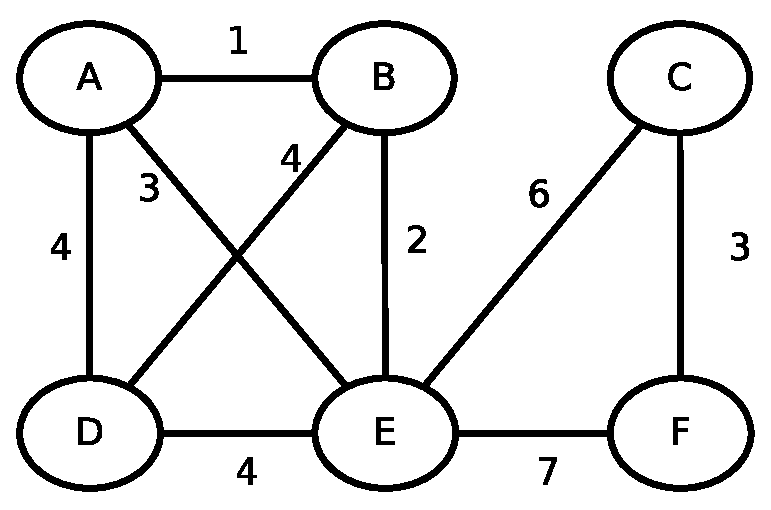
\includegraphics[width=\textwidth]{clustering/mst_graph}
        \caption{Example of a graph.}
        \label{fig:graph}
    \end{subfigure}
    %\hfill
    \hspace{30pt}
    \begin{subfigure}[b]{0.3\textwidth}
        \centering
        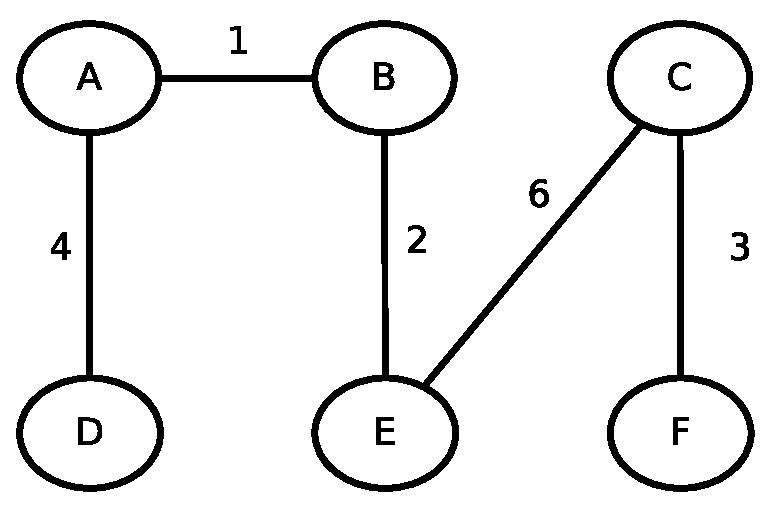
\includegraphics[width=\textwidth]{clustering/mst_mst}
        \caption{MST of the graph to the left.}
        \label{fig:graph mst}
    \end{subfigure}

    \caption{The above figures show an example of a graph (left) and its corresponding Minimum Spanning Tree (right). The circles are vertices and the edges are the lines linking the vertices.}
    \label{fig:mst example}
\end{figure}

An example of a Single-Link dendrogram and resulting cluster can be observed in Fig. \ref{fig:sl plots}.
The dendrogram in Fig. \ref{fig:sl dendrogram} has been truncated to 25 clusters in the bottom level for the sake of readability.
The clustering presented on Fig. \ref{fig:sl clustering} is the result of cutting the dendrogram such that only 3 clusters exist (the number of classes).
The accuracy, as measured by the CI, is of $58\%$.

\begin{figure}[!ht]
    \centering
    \begin{subfigure}[b]{0.45\textwidth}
        \centering
        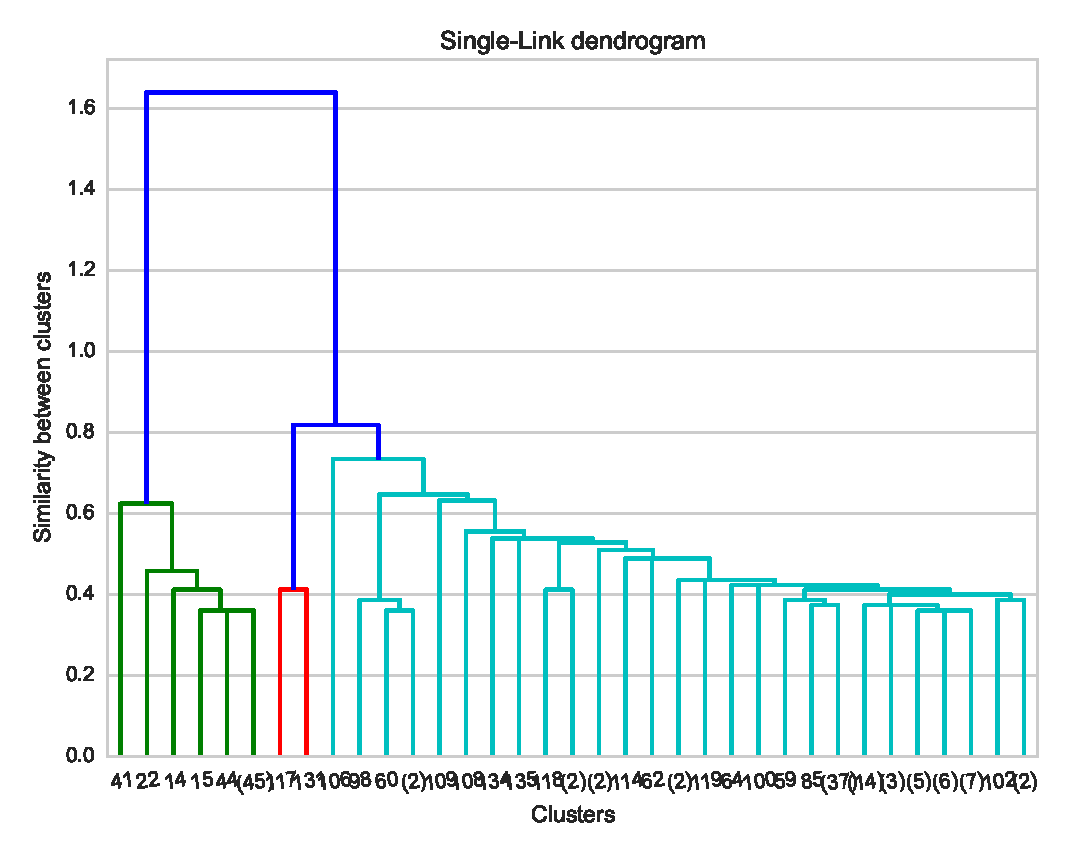
\includegraphics[width=\textwidth]{clustering/sl_dendrogram}
        \caption{Single-Link dendrogram truncated to 25 clusters in the bottom level.}
        \label{fig:sl dendrogram}
    \end{subfigure}
    %\hfill
    \begin{subfigure}[b]{0.45\textwidth}
        \centering
        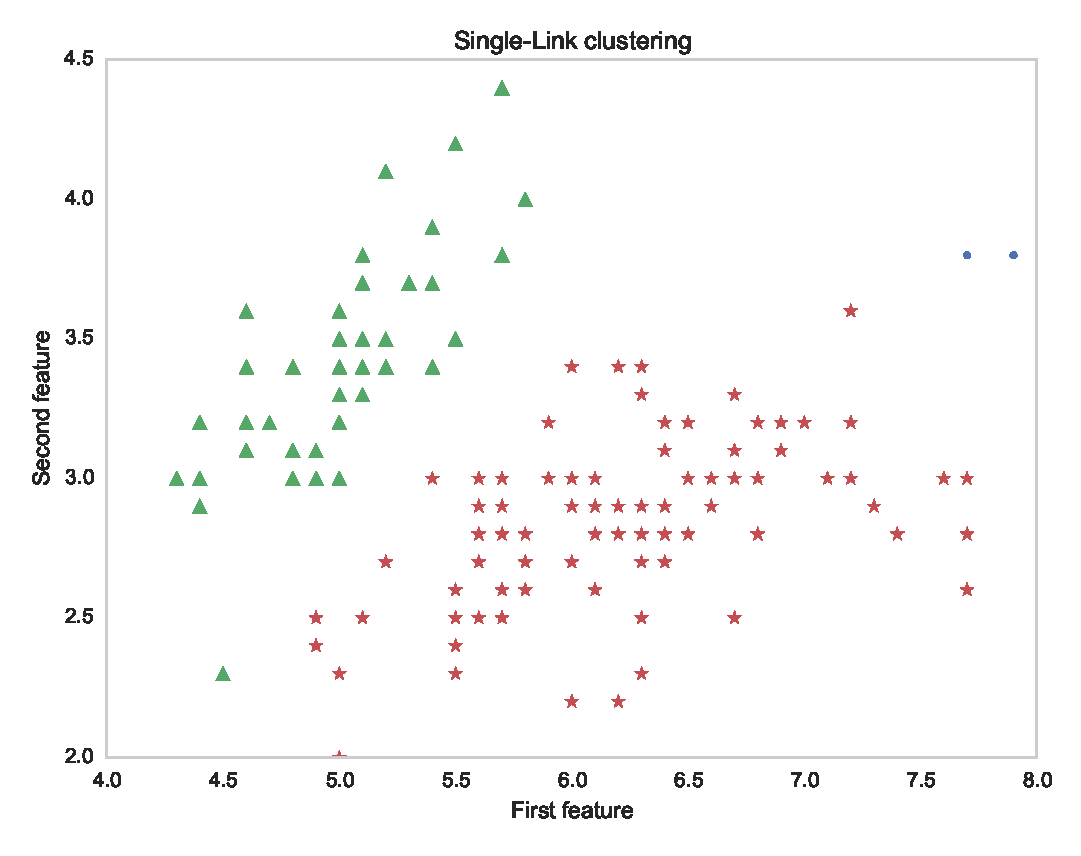
\includegraphics[width=\textwidth]{clustering/sl}
        \caption{Clustering with 3 clusters.}
        \label{fig:sl clustering}
    \end{subfigure}

    \caption{The above plots show the dendrogram and a possible clustering taken from a Single-Link run over the Iris dataset. Fig. \ref{fig:sl clustering} was obtained by performing a cut on a level that would yield a partition of 3 clusters.}
    \label{fig:sl plots}
\end{figure}





% % % % % % % % % % % % % % % % % % % % % % % % % % % % % % % % % % % % % % % %
%
%                   EVIDENCE ACCUMULATION CLUSTERING
%
% % % % % % % % % % % % % % % % % % % % % % % % % % % % % % % % % % % % % % % %

\section{Ensemble Clustering}
\label{sec:ensemble}

The underlying idea behind ensemble clustering is to take a collection of partitions, a \emph{clustering ensemble}, and combine it into a single partition.
There are several motivations for ensemble clustering.
Data from real world problems appear in different configurations regarding shape, cardinality, dimensionality, sparsity, etc. 
Different clustering algorithms are appropriate for different data configurations, e.g. K-Means tends to group patterns in hyperspheres \cite{Jain1999} so it is more appropriate for data whose structure is formed by hypershere like clusters.
If the true structure of the data at hand is heterogeneous in its configuration, a single clustering algorithm might perform well for some part of the data while other performs better for some other part.
Since different partitions are used, one can use a mix of algorithms to address different properties of the data such that the combination is more \textbf{robust} to noise and outliers \cite{topchy2004mixture} and the final clustering has a \textbf{better quality} \cite{Aggarwal2014}.
Even using several partitions from different initializations of the same algorithm may also allow retrieving complex shaped structures from otherwise simple methods.
Ensemble clustering can also be useful in situations where one does not have direct access to all the features of a given dataset but can have access to partitions from different subsets and later combining with an ensemble algorithm.
Furthermore, the generation of the clustering ensemble can be \textbf{parallelized and distributed} since each partition is independent from every other partition.

A clustering ensemble, according to \cite{Fred2005}, can be produced from (1) different data representations, e.g. choice of preprocessing, feature selection and extraction, sampling; or (2) different partitions of the data, e.g. output of different algorithms, varying the initialization parameters on the same algorithm.

% different approaches to ensemble clustering
Ensemble clustering algorithms can take three main distinct approaches \cite{Aggarwal2014}: based on pair-wise similarities, probabilistic or direct.
EAC \cite{Fred2005} and CSPA \cite{Strehl2002} are examples of pair-wise similarity based approach, where the algorithms use a co-associations matrix.
The MMCE \cite{topchy2004mixture} and BCE \cite{wang2011bayesian} are examples of a probabilistic approach.
This approach will be further clarified when the EAC algorithm is explained.
HGPA \cite{Strehl2002}, MCLA \cite{Strehl2002} and bagging \cite{Dudoit2003} are examples of a direct approach to combining the ensemble clusterings, where the algorithms work directly with the labels without creating a co-association matrix.
A detailed and thorough review of the similarity measures that can be used on with clustering ensembles and the state of the art algorithms can be consulted in \cite{Aggarwal2014}.

% Many cluster ensemble algorithms exist, e.g. Bipartite \cite{Hore2009}, Metis Merger \cite{Hore2009}, CSPA \cite{Strehl2002}, HGPA \cite{Strehl2002}, MCLA \cite{Strehl2002} and EAC \cite{Fred2002}.

\section{Evidence Accumulation Clustering}
\label{sec:eac}

\subsection{Overview}

The goal of EAC is to find an optimal partition $P^*$ containing $k^*$ clusters, from the clustering ensemble $\mathbb{P}$. The optimal partition should have the following properties \cite{Fred2005}:

\begin{itemize}
    \item \textbf{Consistency} with the clustering ensemble;
    \item \textbf{Robustness} to small variations in the ensemble; and,
    \item \textbf{Goodness} of fit with ground truth information, when available.
\end{itemize}

\emph{Ground truth} is the true labels of each sample of the dataset, when such exists, and is used for validation purposes.
Since EAC is an unsupervised method, this typically will not be available.
EAC makes no assumption on the number of clusters in each data partition.
Its approach is divided in 3 steps:

\begin{enumerate}
\item \textbf{Production} of a clustering ensemble $\mathbb{P}$ (the evidence);
\item \textbf{Combination} of the ensemble into a co-association matrix;
\item \textbf{Recovery} of the natural clusters of the data.
\end{enumerate}

% introduce the creation of the ensemble
In the first step, a clustering ensemble is produced.
Within the context of EAC, it is of interest to have variety in the ensemble with the intention of better capturing the underlying structure of the data.
One such parameter to measure that variety is the number of clusters in the partitions of the ensemble.
Typically, the number of clusters in each partition is drawn from an interval $[K_{min}, K_{max}]$ with uniform probability.
This influences other properties of other parts of the algorithm such as the sparsity of the co-association matrix as will become clearer in future chapters.
Reviewing the literature \cite{Fred2002,Fred2005,Lourenco2007,lourenco2014ecg}, it is clear the ensemble is usually produced by random initialization of K-Means (specifying only the number of centroids within the above interval).
Still, other clustering algorithms have been used for the production of the ensemble \cite{Duarte2005} such as Single-Link, Average-Link and CLARANS.

The ensemble of partitions is combined in the second step, where a non-linear transformation turns the ensemble into a co-association matrix \cite{Fred2005}, i.e. a matrix $\mathcal{C}$ where each of its elements $n_{ij}$ is the association value between the pattern pair $(i,j)$.
The association between any pair of patterns is given by the number of times those two patterns appear clustered together in any cluster of any partition of the ensemble, i.e. the number of co-occurrences in the same cluster.
The rationale is that pairs that are frequently clustered together are more likely to be representative of a true link between the patterns \cite{Fred2002}, revealing the underlying structure of the data.
In other words, a high association $n_{ij}$ means it is more likely that patterns $i$ and $j$ belong to the same class.
The construction of the co-association matrix is at the very core of this method.

The co-association matrix itself is not the output of EAC.
Instead, it is used as input to other methods to obtain the final partition.
The co-association between any two patterns can be interpreted as a similarity measure.
Thus, since this matrix is a similarity matrix it's appropriate to use algorithms that take this type of matrices as input, e.g. K-Medoids or hierarchical algorithms such as Single-Link or Average-Link, to name a few.
Typically, algorithms use a distance as the dissimilarity, which means that they minimize the distance to obtain the highest similarity between objects.
However, a low value on the co-association matrix translates in a low similarity between a pair of objects, which means that the co-association matrix requires prior transformation for accurate clustering results, e.g. replace every similarity value $n_{ij}$ between every pair of object $(i,j)$ by $max \{ \mathcal{C} \} - n_{ij}$.

Although any algorithm can be used, the final clustering is usually done using SL or AL.
Each of these algorithms will take as input the transformed co-association matrix as the dissimilarity matrix.
Furthermore, not knowing the "natural" number of clusters one can use the lifetime criteria.
The k-cluster lifetime is defined by \citet{Fred2005} as the range of threshold values on the dendrogram that lead to the identification of k clusters.
The lifetime criteria chooses the longest lifetime as the threshold interval where a cut in the dendrogram should be made so as to produce a partition.
In other words, the number of clusters $k$ should be such that it maximizes the cost of cutting the dendrogram from $k-1$ clusters to $k$.


% paragraph on weighted EAC: Weighting Cluster Ensembles in Evidence Accumulation Clustering
Related work to EAC has been developed.
The Weighted EAC (WEAC) algorithm \cite{Duarte2005} and a study on the sparsity of the co-association matrix \cite{Lourenco2010} should be mentioned.
The latter is discussed in more depth in chapter \ref{chapter:stateofart}.
The former introduces the novelty of having weights associated to each partition such that good quality partitions are more relevant than their counterparts.
These weights are based on internal validity measures.
Weighing the partitions in terms of quality has shown to improve the original algorithm, accuracy wise.


%examples of applications
EAC has been used with success in several areas.
To name a few, it was used for the automatic identification of chronic lymphocyt leukemia \cite{Qian2010}, for the unsupervised analysis of ECG-based biometric database to highlight natural groups and gain further insight \cite{lourenco2014ecg} and as a solution to the problem of clustering of contour images (from hardware tools) \cite{Lourenco2007}.

% \subsection{Advantages and Disadvantages}
% %#REVIEW advantages and disadvantages of EAC

% An advantage of EAC is that it takes no input parameters such as the number of output clusters.
% Furthermore, it provides good accuracy on datasets with hard shapes \cite{Fred2005}.
% On the other hand, a big disadvantage is space complexity of the evidence combination step.
% In this step, when using the standard EAC, a co-association matrix is build, resulting in a complexity of $O(N^2)$.
% This translates in an almost prohibitive use of this method for bigger datasets.
 % file "Thesis_Introduction.tex"
%!TEX root = Thesis.tex

\chapter{State of the art}
\label{chapter:stateofart}

% Na reunião em do feedback do relatório tinha-se falado em ter o overview do EAC no capítulo de nomenculatura e conceitos de clustering (que também irá incluir o K-Means e o single link). No entanto, tendo que estes dois algorithmos são "clássicos" e o EAC é state-of-the-art não faria sentido ter a explicação do EAC logo no inicio do capítulo State of the Art?

% A ideia seria então começar por explicar o EAC. Depois disso, rever o que foi feito em termos de escalibilidade do mesmo. Depois ter uma secção de Big Data em que basicamente se mostraria o que pode ser feito nesta área (ou talvez ter esta secção antes da escalibilidade do EAC). E só depois poria as secções do quantum clustering e do conceito e algoritmos GPU.


% motivation
Scalability of EAC to large datasets is the concern of this work and, because of that, this chapter starts by reviewing what has been done in terms of scaling EAC in section \ref{sec:eac scaling}.
EAC is a method of three parts and this dissertation is concerned with the scalability of the whole algorithm which means that each step must be optimized.
Scaling an algorithm means one has to take into account both speed of execution and memory requirements.
Increasing speed can be attained with either faster algorithms and/or faster computation of existing algorithms.
% Both these approaches to faster generation of the ensemble were pursued and researched.
This chapter reflects research done within both approaches.

% EAC section
% Before reviewing methods and techniques relevant for scaling EAC, this chapter starts by presenting the state of the art of EAC and related research in section \ref{sec:eac}.
% This section provides a brief overview of ensemble clustering, explains the EAC algorithm, refers to where it has been applied and reviews what has been done in terms of scaling it.

% large datasets section
Although research on the application of EAC to large datasets has not been pursued before, cluster analysis of large datasets has. 
Since EAC uses traditional clustering algorithms (e.g. K-Means, Single-Link) in its approach, it is useful to understand how scalable the individual algorithms are as they will have a big impact in the scalability of EAC.
Furthermore, valuable insights may be taken from the techniques used in the scalability of other algorithms.
To this end, section \ref{sec:big data} presents a brief review on cluster analysis of large datasets, with a focus on parallelization with GPUs.
Furthermore, it offers a more detailed description of a GPU parallel version of K-Means and an approach for parallelizing Single-Link with the GPU.

% quantum clustering
An alternative approach on clustering for scaling with faster algorithms, the still young field of quantum clustering, was reviewed in section \ref{sec:quantum clustering}.
This line of research was taken mostly with the first step of EAC in mind.


% The former in the form of the still young field of quantum clustering, which is briefly reviewed in section , and the latter in the field of parallel computation, more specifically on computation in GPUs, reviewed in section \ref{sec:gpgpu}.
% While quantum clustering was only reviewed for the first step, the parallel computation paradigm was investigated with all steps in mind.
% For that reason, K-Means GPU versions were researched as well as a MST-based Single Linkage Clustering method.

% % % % % % % % % % % % % % % % % % % % % % % % % % % % % % % % % % % % % % % %
%
%  					EAC SCALABILITY
%
% % % % % % % % % % % % % % % % % % % % % % % % % % % % % % % % % % % % % % % %


\section{Scalability of EAC}
\label{sec:eac scaling}
The quadratic space and time complexity of processing the $n \times n$ co-association matrix is an obstacle to an efficient scaling of EAC.
Two approaches have been proposed to address this obstacle: one dealing with reducing the co-association matrix by considering only the distances of patterns to their $p$ neighbors and the other by using a sparse co-association matrix and maximizing its sparsity.

\subsection{$p$ neighbors approach}
The first approach, \cite{Fred2005}, proposes an alternative $n \times p$ co-association matrix, where only the $p$ nearest neighbors of each pattern are considered in the evidence combination step.
This comes at the cost of having to keep track of the neighbors of each pattern in a separate data structure of $O(np)$ memory complexity and also of pre-computing the $p$ neighbors, which has a time complexity of $O(n^2)$ to compute the proximity measure from each pattern to every other pattern.
The quadratic space complexity of the co-association matrix is then transformed to $O(2np)$: $O(np)$ for the actual co-association matrix and $O(np)$ for keeping track of the neighbors.
Since usually one has $p < \frac{n}{2}$ (value for which both this approach and the original $n \times p$ matrix would take the same space), the cost of storing the extra data structure is lower than that of storing an $n \times n$ matrix, e.g. for a dataset with $10^6$ patterns and $p=\sqrt{10^6}$ (a value much higher than the $20$ neighbors used in \cite{Fred2005}), the total memory required for the co-association matrix would decrease from $3725.29 GB$ to $7.45 GB$ ($0.18\%$ of the memory occupied by the complete matrix).
% However, it should be noted that computing the $p$ nearest neighbors requires the computation of $n^2$ distance values.

\subsection{Increased sparsity approach}
The second approach, presented in \cite{Lourenco2010}, exploits the sparse nature of the co-association matrix.
The co-association matrix is symmetric and with a varying degree of sparsity.
The former property translates in the ability of storing only the upper triangular of the matrix without any loss on the quality of the results.
The latter property is further studied with regards to its relationship with the minimum $K_{min}$ and maximum $K_{max}$ number of clusters in the partitions of the input ensemble.
The core of this approach is to only store the non-zero values of the upper triangular of the co-association matrix.
The authors study 3 models for the choice of these parameters:

\begin{itemize}
	\item choice of $K_{min}$ based on the minimum number of gaussians in a gaussian mixture decomposition of the data;
	\item based on the square root of the number of patterns ($\{K_{min},K_{max}\} = \{\frac{\sqrt{n}}{2},\sqrt{n}\}$);
	\item or based on a linear transformation of the number of patterns ($\{K_{min},K_{max}\} = \{\frac{n}{A},\frac{n}{B}\},A<B$).
\end{itemize}

where $A$ and $B$ are two suitable constants chosen by the researcher.
The study compared the impact of each model in the sparsity of the co-association matrix (and, thus, the space complexity) and in the relative accuracy of the final clusterings.
Both theoretical predictions and results revealed that the linear model produces the highest sparsity in the co-association matrix, under a dataset consisting of a mixture of Gaussians.
Furthermore, it is true for both linear and square root models that the sparsity increases as the number of samples increases.

For real datasets, the performance of the three models became increasingly similar with the increase of the cardinality of the problem.
It was found that the chosen granularity of the input partitions ($K_{min}$) is the variable with most impact, affecting both accuracy and sparsity.
The authors reported this technique has linear space and time complexity on benchmark data.

The number of samples of the datasets analysed in \cite{Lourenco2010} was under $10^4$.
Furthermore, it should be noted that the remarks concerning the sparsity of the co-association matrix in the aforementioned study refer to the number of non-zero elements in the matrix and does not take into account extra data structures that accompany real sparse matrices implementations.

% Although the results appear promising, the present work aims to deal with datasets much larger than this and, as a consequence, this technique should be further evaluated and tested to attest to its usefulness to very large datasets. %TODO: this paragraph is probably more relevant in the methodology section so as to introduce why other techniques were necessary


% % % % % % % % % % % % % % % % % % % % % % % % % % % % % % % % % % % % % % % %
%
%  					BIG DATA CLUSTERING
%
% % % % % % % % % % % % % % % % % % % % % % % % % % % % % % % % % % % % % % % %

\section{Clustering with large datasets}
\label{sec:big data}

% \subsection{The concept of Big Data}
% % there is a difference between this and the big data section in the state of the art chapter
% % here we are dealing with the big data paradigm, an overview of what is, what has been happening
% % I'm trying t justigy why big data is an interesting 
% % most focus should into the problems themselves and why they are interesting

% examples of success application

% characteristics and challenges
% \subsection{Computation in Big Data}

% this is probably good for motivating this section in the introduction of the chapter
% Scalability of EAC within the big data paradigm is the concern of this work.
% Although this line of research has not been pursued before, cluster analysis of large datasets has.
% Since EAC uses traditional clustering algorithms (e.g. K-Means, Single-Link) in its approach, it is useful to understand how scalable the individual algorithms are as they will have a big impact in the scalability of EAC.
% Furthermore, valuable insights may be taken from the techniques used in the scalability of other algorithms.


%this was taken from the Data Clustering: Algorithms and Applications book

% introcution for big data clustering
When large datasets, and big data, is in discussion, two perspectives should be taken into account \cite{Aggarwal2014}.
The first deals with the applications where data is too large to be stored efficiently.
This is the problem that streaming algorithms such as LOCALSEARCH \cite{bigdatastream} try to solve by analyzing data as it is produced, close to real-time processing.
The other perspective is data that is actually stored for later processing which is the perspective relevant to the present work and will be further discussed below.

% different approaches on big data clustering
The flow of clustering algorithms typically involves some initialization step (e.g. choosing the number of centroids in K-Means) followed by an iterative process until some stopping criteria is met, where each iteration updates the clustering of the data \cite{Aggarwal2014}.
In light of this, to speed up and/or scale up an algorithm, three approaches are available: (1) reduce the number of iterations, (2) reduce the number of patterns and/or features to process or (3) parallelizing and distributing the computation.
The solutions for each of these approaches are, respectively, one-pass algorithms (e.g. CLARANS \cite{ng2002clarans}, BIRCH \cite{zhang1996birch}, CURE \cite{guha1998cure}), randomized techniques that reduce the input space complexity (e.g. PCA, CX/CUR \cite{drineas2006fast}) and parallel algorithms (parallel K-Means \cite{Zechner2009b}, parallel spectral clustering \cite{chen2011parallel}).

% another example for randomized techniques that reduce input space complexity: local-preserving projection \cite{johnson1984extensions};
% CX/CUR is a global projection

% parallelization approach to big data clustering
Parallelization can be attained by adapting algorithms to multi core CPU, GPU, distributed over several machines (a \emph{cluster}) or a combination of the former, e.g. parallel and distributed processing using GPU in a cluster of hybrid workstations.
Each approach has its advantages and disadvantages.
% CPU
The CPU approach has access to a larger memory but the number of computation units is reduced when compared with the GPU or cluster approach.
Furthermore, CPUs have advanced techniques such as branch prediction, multiple level caching and out of order execution - techniques for optimized sequential computation.
% GPU
GPU have hundreds or thousands of computing units but typically the available device memory is reduced which entails an increased overhead of memory transfer between host (workstation) and device (GPU) for computation of large datasets.
In addition, it is harder to scale the above solutions for even bigger datasets.
On the other hand, GPUs can be found on a large variety of computing platforms, from mobile devices to workstations and datacenters.
% clusters
A cluster offers a parallelized and distributed solution, which is easier to scale.
According to \cite{Aggarwal2014}, the two algorithmic approaches for cluster solutions are (1) memory-based, where the problem data fits in the main memory of the machines of the cluster and each machine loads part of the data; or (2) disk-based, comprising the widely used MapReduce framework capable of processing massive amounts of data in a distributed way.
The main disadvantage is that there is a high communication and memory I/O cost to pay.
Communication is usually done over the network with TCP/IP, which is several orders of magnitude slower than the direct access of the CPU or GPU to memory (host or device).

% overview of the section; motivation for GPU K-Means and GPU SL/MST
The present work is oriented towards GPU based parallelization, since GPUs are an easily accessible commodity and the goals of the dissertation are oriented towards computation on a single machine.
Taking that into consideration, this section reviews a GPU parallel version of the K-Means algorithm and goes on to describe a GPU parallel approach for performing Single-Link clustering.
For an overview of General Purpose computing in GPUs (GPGPU), the reader is referred to Appendix A.
% Taking that into consideration, this section starts by covering a review of the General Purpose computing on GPUs paradigm.
% It goes on to review a GPU parallel version of the K-Means algorithm and a GPU parallel approach for performing Single-Link clustering.


\subsection{Parallel K-Means}
\label{sec:art parallel kmeans}

K-Means is an obvious candidate to generate the ensemble of the first step of EAC because it uses different initializations and parameters and due to its simplicity.
Besides, K-Means is a very good candidate for parallelization.
Still, other algorithms can be used to produce ensembles.

% As explained in chapter \ref{chapter:clustering}, K-Means has two main steps: labeling and update.

Several parallel implementations of this algorithm for the GPU exist \cite{Bai2009, Wu2011, Zechner2009, Sirotkovi2012, Farivar2008} and all report significant speed-ups relative to their sequential counterparts in certain conditions, usually after the input dataset goes above a certain cardinality, dimensionality or number of clusters threshold.
The first step is inherently parallel as the computation of the label of the $i$-th pattern is not dependent on any other pattern, but only on the centroids.
Two approaches to parallelize this step on the GPU are possible, a centroid-centric or a data-centric \cite{Bai2009}.
In the former each thread is responsible for a centroid and will compute the distance from its centroid to every pattern.
These distances must be stored and, in the end, the patterns are assigned to the closest centroid.
In the latter, each thread will compute the distance from one or more data points to every centroid and determines to which centroid they are closest.
This strategy has the advantage of using less memory since it does not need to store all the pair-wise distances to perform the labeling - it only needs to store the best distance for each pattern.
According to \cite{Bai2009}, the former approach is suitable for devices with a low number of cores so as to stream the data to each one, while the latter is better suited to devices with more cores.

The approach taken in \cite{Zechner2009b} only parallelizes the labeling stage and takes a data-centric approach to the problem.
Each thread computes the distance from a set of data points to every centroid and determines the labels.
The remaining steps are performed by the host CPU.
This study reported speed-ups up to 14, for input datasets of $500\:000$ points.
Furthermore, it should be noted that the speed up was measured against a sequential version with all C++ compiler optimizations turned on, including vector operations (which, by themselves, are a way of parallelizing computation).
The parallelized algorithm's flow can be observed in Figure \ref{fig:kmeans}.

\begin{figure}[hbtp]
	\centering
	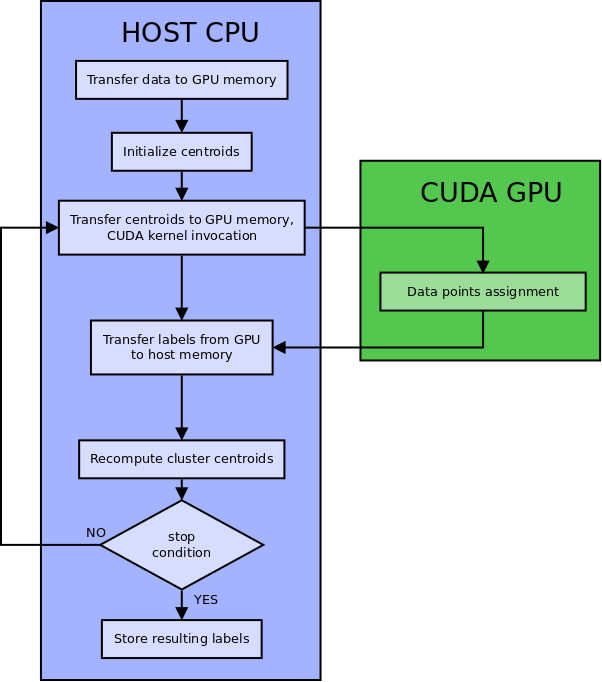
\includegraphics[width=0.7\textwidth]{stateofart/gpgpu/kmeans}
	\caption{Flow execution of the GPU parallel K-Means algorithm.}
	\label{fig:kmeans}
\end{figure}

The implementation of \citet{Zechner2009b} uses one thread per data point.
Each centroid is transfered to shared memory and each thread will compute the distance from its data point to the centroid.
Moreover, the data point is fetched from global memory in a coalesced manner.

It should be noted that the literature reports that the performance of K-Means using Dynamic Parallelism is slightly worse than its standard GPU counterpart \cite{DiMarco2013}.
% The results of aforementioned study showed datasets sufficiently large to make them relevant for the present work, considering the focus of the dissertation. 

\subsection{Parallel Single-Link Clustering}
\label{sec:parallel_SL}

Single-Link (SL) is an important step in the EAC chain.
Given the new similarity metric (how many times a pair of patterns are clustered together in the ensemble), SL provides an intuitive way of obtaining the final partition: patterns that are clustered together often in the ensemble should remain clustered together in the final solution.

% explain how SL works -> is done in the clusteirng chapter
% The sequential SL algorithm works over a pair-wise similarity matrix and starts by considering that every data point is a separate cluster.
% Then, in each iteration, it selects the smallest weight that connects two clusters and merges the two clusters.
% The algorithm stops when $n-1$ merges have been performed, which is when all the data points have been connected in the same cluster.
% The output is a dendrogram connecting all the data points at different levels.

% SL link to MST
SL is not easily parallelized since a new cluster generated at each step may include the one generated in the previous iteration.
The most parallelizable part is the computation of the pair-wise similarity matrix, which is only useful if the input is raw data instead of a similarity matrix as in the case of EAC.
%, which in EAC is computed with the part of the input (the co-association matrix) and, thus, not considered.
The relationship between SL and the Minimum Spanning Tree, explained in chapter \ref{chapter:clustering}, is the key to parallelize it.
If one takes this approach for solving the SL problem, it becomes easier to parallelize it since parallel MST algorithms are abundant in literature \cite{Vineet2009,rostrup2013fast,Sousa2015}.
The same approach for extracting the final clustering in EAC was used in \cite{Fred2002}.

% An important relationship between SL and the Minimum Spanning Tree problem of graphs is the key to parallelize SL.
% If one takes the pair-wise similarity matrix to be a graph (each pattern is a node and each association an edge), then, when performing SL over this graph, the result can be interpreted as a structured MST.
% To get $n$ clusters, one cuts the $n-1$ links with highest cost.
% Furthermore, the MST approach to solve SL has been reported to be among the fastest solutions, since (1) it needs only $O(n)$ working space instead of the $O(n^2$ space of a pair-wise similarity matrix working copy and (2) it reads each similarity only once \cite{Mullner2011}.
% It should be noted that another algorithm with the characteristics mentioned for the MST approach for SL exist in another algorithm, the SLINK \cite{Sibson1973}, which even has some advantages under certain conditions \cite{Mullner2011}.

\subsubsection{Algorithm for finding Minimum Spanning Trees}
There are several algorithms for computing an MST.
The most famous are Kruskal \citep{kruskal1956shortest}, Prim \citep{prim1957shortest} and Borůvka \citep{boruuvka1926jistem}.
Borůvka's algorithm is also known as Sollin's algorithm.
The first two are mostly sequential, while the latter has the highest potential for parallelization, specially in the first iterations.
As such, even though GPU parallel variants of Kruskal's \citep{rostrup2013fast} and Prim's \citep{Wang2011} algorithms exist, the focus will be on Borůvka's.% (which was also the first to be parallelized for the GPU).

Several parallel implementations of this algorithm for the GPU exist, e.g. \citep{Vineet2009}, \cite{harish2009large} and \citep{Sousa2015}. \citet{Sousa2015} provides a more in-depth review over the current state of the art of MST solvers for the GPU and proposes an algorithm reported to be the fastest.
This section will review the algorithm proposed in \citep{Sousa2015}, referred to as \emph{Sousa2015} from henceforth.

%some graph theory and graph representation
Since this algorithm operates over graphs, relevant graph notation is introduced here.
In graph theory, a graph $G = (V,E)$ is composed by a set of vertices $V$ and a set of edges $E$ connecting those vertices.
Furthermore, if $G$ is a connected graph, then there is a path between any $s,t \in V$.
An example of a graph can be observed in Fig. \ref{fig:mst example} of chapter \ref{chapter:clustering}, where the MST was first introduced.
A $|V| \times |V|$ matrix can fully represent a graph if one takes each element $(i,j)$ of the matrix to be the weight of the edge connecting vertices $i$ and $j$.
Typically, a graphs is not fully connected (vertices connected to all the other vertices), which means that the matrix is often sparse.

\subsubsection{CSR format}
\emph{Sousa2015} takes in a graph as input, represented in the CSR format (a format used for sparse matrices).
This representation is equivalent to having a square matrix $G$ with zeroed diagonal where the $g_{ij}$ element of the matrix is the weight of the link connecting the node $i$ with the node $j$.
This format is represented in Fig. \ref{fig:csr}.
It requires three arrays to fully describe the graph:

\begin{itemize}
	\item a \emph{data} array containing all the non-zero values, where values from the same row appear sequentially from left to right and top to bottom, i.e. in \emph{row-major} order, e.g. if the first row has 20 non-zero values, then the first 20 elements from this array belong to the first row;
	\item an \emph{indices} array of the same size as \emph{data} containing the column index of each non-zero value;
	\item an \emph{indptr} array of the size of the number of rows containing a pointer to the first element in the \emph{data} and \emph{indices} arrays that belongs to each row, e.g. if the $i-th$ element (row) of \emph{indptr} is $k$ and it has 10 values, then all the elements from $k$ to $k + 10$ in \emph{data} belong to the $i-th$ row.
\end{itemize}

\begin{figure}[hbtp]
\centering
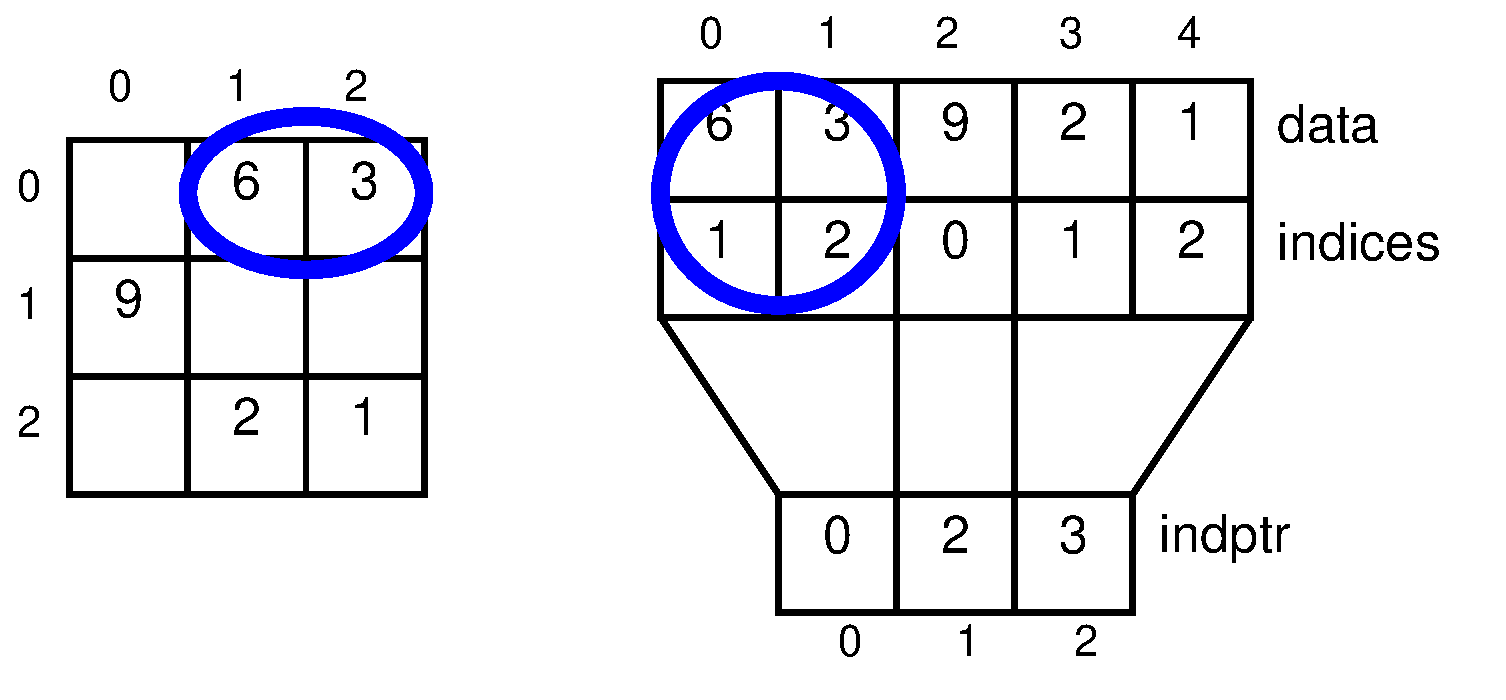
\includegraphics[width=0.5\textwidth]{stateofart/gpgpu/csr_format}
\caption{Correspondence between a sparse matrix and its CSR counterpart.}
\label{fig:csr}
\end{figure}

Within the algorithm's context, these three arrays are denominated as \emph{first\_edge}, \emph{destination} and \emph{weight}, respectively.
There change in denomination is for making their purposes clearer.
Although these three arrays can completely describe a graph, the algorithm uses an extra array \emph{outdegree} that stores the number of non-zero values of each row and can be deduced from the \emph{first\_edge} array.

The length and purpose of each of these arrays are:
\begin{itemize}
	\item \emph{first\_edge} is an array of size $|V|$, where the \emph{i-th} element points to the first edge corresponding to the \emph{i-th} vertex.
	\item \emph{outdegree} is an array of size $|V|$, where the \emph{i-th} element contains the number of edges attached to the \emph{i-th} vertex.
	\item \emph{destination} is an array of size $|E|$, where the \emph{j-th} element points to the destination vertex of the \emph{j-th} edge.
	\item \emph{weight} is an array of size $|E|$, where the \emph{j-th} element contains the weight of the \emph{j-th} edge.
\end{itemize}

$|V|$ is the number of vertices and $|E|$ is the number of edges.
The number of edges is duplicated to cover both directions, since the algorithm works with undirected graphs.
This basically means that instead of using the the upper (or lower) triangular matrix (which can also completely describe the graph), it uses a complete matrix resulting in double redundancy of each edge.
The edges in the \emph{destination} array are grouped together by the vertex they originate from, e.g. if edge $j$ is the first edge of vertex $i$ and this vertex has 3 edges, then edges $\{j,j+1,j+2\}$ are the outgoing edges of vertex $i$ and are stored sequentially in the \emph{destination} array.

\subsubsection{Steps of the algorithm}

Within the context of the algorithm the \emph{id} of a vertex is its index in the \emph{first\_edge} array, the \emph{color} represents a component and is the \emph{id} of the component representative and the \emph{successor} of a vertex is the destination vertex of one of its edges.
One should keep in mind this is a parallel algorithm and each of its steps is computed concurrently.
Except for the \emph{exclusive prefix sum}, each thread processes a single vertex and each computation is usually independent.
In some steps, however, threads need to access the same resource and it is important the state of the resource does not change in the middle of the operation that accesses it.
In these cases, atomic operations (operation that are guaranteed to be isolated and, thus, not interruptible) are used.
The algorithm's flow is presented in Figure \ref{fig:mst sousa} and its main steps are explained below.

%maybe have the figures from the paper here to illustrate the process?
\begin{enumerate}
	\item \emph{Find minimum edge per vertex}: select and store the minimum weighted edge for each vertex and resolve same weight conflict by picking the edge with lower destination vertex id.

	\item \emph{Remove mirrored edges}: an edge is mirrored if the successor of its the destination vertex is the origin vertex, e.g. if vertex 1 points to vertex 2 and vertex 2 points back to vertex 1.
	% a mirrored edge the successor of its destination vertex is its origin vertex.
	All mirrored edges are removed from the selected edges in the first step. All edges that are not removed are added to the resulting MST.

	\item \emph{Initialize and propagate colors}: this step is responsible for identifying connected components so the graph may be contracted.
	Each connected component will be a super-vertex in the contracted graph, which means it will be a single vertex representing a subgraph.
	Each vertex is initialized with the same color of its successor's id.
	If a vertex has no successor because that edge was removed in the previous step, then it will be the representative vertex of the component and its color is initialized with its own id.
	The colors are then propagated by setting each vertex's color to the color of its successor, until convergence.

	\item \emph{Create new vertex ids}: only the super-vertices will be propagated to the next iteration but they will have new ids for building the new contracted graph.
	The new ids will range from $0$ to $s$, where $s$ is the number of super-vertices.
	% The vertex that will represent a super-vertex is the vertex whose color has its own id.
	The vertices representing a super-vertex (component) will take the new ids in increasing order according to their own ids in increasing order, e.g. vertex $2$ is the representative with lowest id so it will have the id $0$ in the contracted graph.
	This step relied on the \emph{exclusive scan} operation, which is explained in section \ref{sub:scan}.

	\item \emph{Count, assign, and insert new edges}: the final step consists in building the contracted graph.
	The algorithm will count the number of edges connecting each super-vertex to other super-vertices, i.e. the connections between subgraphs.
	This is simply accomplished by selecting every edge whose origin and destination colors are distinct.
	For each such edge the corresponding positions of the origin and destination super-vertices in a new \emph{outdegree} array are incremented with an atomic operation.
	The new \emph{first\_edge} array is obtained from performing an exclusive scan over \emph{outdegree}.
	The next step is to assign and insert edges in the contracted graph.
	Once again, the algorithm will determine which edges will be in the contracted graph by checking the origin and destination colors.
	A copy, called \emph{top\_edge}, of the new \emph{first\_edge} array will track of where to insert the new edges.
	When an edge is assigned to a super-vertex it is inserted in the new \emph{weight} and \emph{destination} arrays composing the contracted graph.
	The position of insertion is specified by \emph{top\_edge} and the algorithm increments \emph{top\_edge} atomically so the next edge will not overwrite the previous one.
	The increment is done with an atomic operation since multiple edges can be assigned to the same super-vertex and the insertion of all edges is being done in parallel.
	It should be noted that duplicated edges are not removed, i.e. several distinct connections between two super-vertices can be kept, since the author considers that the benefit of doing so does not outweigh the computational overhead.
\end{enumerate}

\begin{figure}[hbtp]
\centering
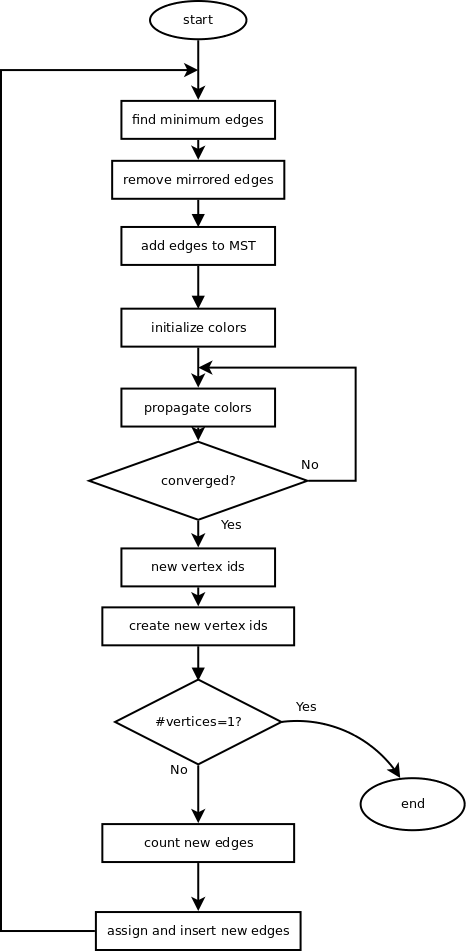
\includegraphics[width=0.5\textwidth]{stateofart/gpgpu/mst_boruvka_flow}
\caption{Flow execution of Sousa2015.}
\label{fig:mst sousa}
\end{figure}

It should be noted, however, that this algorithm does not support unconnected graphs, i.e., it is not able to output a forest of MSTs.
%Upon contact, the author reported that 
A solution to that problem is, on the step of building the flag array, only mark a vertex if it is both the representative of its supervertex and has at least one neighbour.

\subsubsection{Exclusive scan}
\label{sub:scan}
%Algorithm 1 assumes that there are as many processors as data elements. For large arrays on a GPU running CUDA, this is not usually the case. Instead, the programmer must divide the computation among a number of thread blocks that each scans a portion of the array on a single multiprocessor of the GPU. Even still, the number of processors in a multiprocessor is typically much smaller than the number of threads per block, so the hardware automatically partitions the "for all" statement into small parallel batches (called warps) that are executed sequentially on the multiprocessor. An NVIDIA 8 Series GPU executes warps of 32 threads in parallel. Because not all threads run simultaneously for arrays larger than the warp size, Algorithm 1 will not work, because it performs the scan in place on the array. The results of one warp will be overwritten by threads in another warp.

%To solve this problem, we need to double-buffer the array we are scanning using two temporary arrays. Pseudocode for this is given in Algorithm 2, and CUDA C code for the naive scan is given in Listing 39-1. Note that this code will run on only a single thread block of the GPU, and so the size of the arrays it can process is limited (to 512 elements on NVIDIA 8 Series GPUs). Extension of scan to large arrays is discussed in Section 39.2.4.

The \emph{scan} operation is one of the fundamental building blocks of parallel computing. 
Furthermore, two of the steps of the Borůvka variant of \cite{Sousa2015} are performed with an exclusive scan where the operation is a sum. 
To illustrate the functioning of the exclusive scan, let us consider the particular case where the operation of the scan is the sum and the identity (the value for which the operation produces the same output as the input) is naturally $0$.
An example of this operation is presented in Fig. \ref{fig:exprefix sum}.

\begin{figure}[hbtp]
\centering
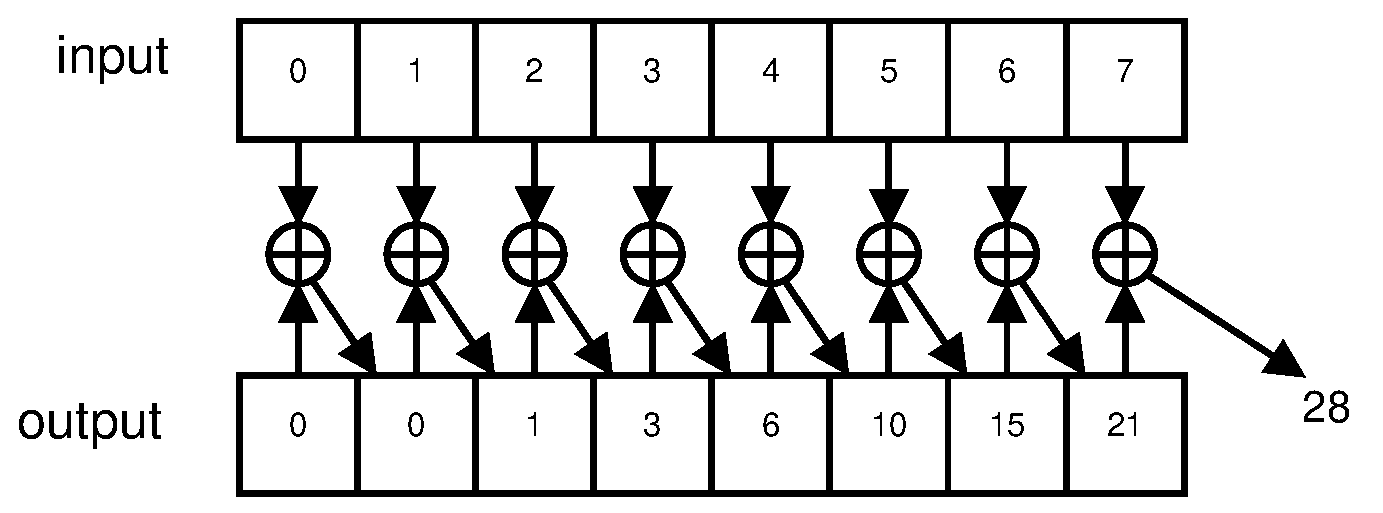
\includegraphics[width=0.5\textwidth]{stateofart/gpgpu/exprefix_sum}
\caption{Example of the exprefix sum operation.}
\label{fig:exprefix sum}
\end{figure}

The first element of the output will be the identity (if it were an inclusive scan, it would be the first element itself).
The second element is the sum between the first element of the input array and the first element of the output array, etc.
The nature of this algorithm seems highly sequential, since each element of the output array depends on the previous one, but two main parallel versions can be found in literature: \citet{Hillis1986} and \citet{Blelloch1990}. 
The two approaches focus on distinct efforts.
The former focuses on optimizing the number of steps \cite{Hillis1986}, has a work complexity of $O(nlogn)$ and a step complexity of $O(logn)$.
The latter focuses on optimizing the amount of work done \cite{Blelloch1990}, has a work complexity of $O(n)$ and a step complexity of $O(2logn)$.
The focus of this dissertation will be on the Blelloch's algorithm.
The reason for this is that the main objective is to deal with very large datasets which guarantees that there will be more work to be done (operations on the data) than there will be available computing resources (streaming processors in the GPU in this case).
When there is more work than processors, one wants to minimize the total amount of work.
On the other hand, when there is more processors than work, one wants to minimize the amount of steps of the algorithm as this translates in the biggest increase in speed.


% HIlli and Steele complexities: $nlogn$ work (operations) and $logn$ steps
% Blelloch complexities: $2n$ work and $2logn$ steps

Blelloch's algorithm is comprised by two main phases: the \emph{reduce phase} (or \emph{up-sweep}) and the \emph{down-sweep phase}.
The algorithm is based on the concept of \emph{balanced binary trees} \cite{Harris2007}, but it should be noted that no such data structure is actually used.
An in-depth explanation of this concept and how it relates to the algorithm falls outside the scope of the present work and it is recommended that the reader consult \cite{Harris2007} or \cite{Blelloch1990} for such details.

During the reduce phase (see Figure \ref{fig:scan reduce}), the algorithm traverses the tree and computes partial sums at the internal nodes of the tree.
This operation is also known as a parallel reduction due to the fact that the total sum is stored in the root node (last node) of the tree \cite{Harris2007}.

\begin{figure}[hbtp]
\centering
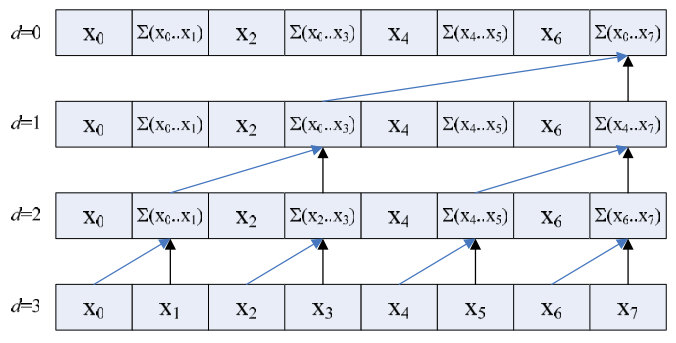
\includegraphics[width=0.8\textwidth]{stateofart/gpgpu/blelloch_reduce}
\caption{Representation of the reduce phase of Blelloch's algorithm \cite{Harris2007}. \emph{d} is the level of the tree and the input array can be observed at $d=0$.}
\label{fig:scan reduce}
\end{figure}

In the down-sweep phase (see Figure \ref{fig:scan down-sweep}) the algorithm traverses back the tree.
During the traversal, and using the partial sums calculated in the reduce phase, it builds the scan in place (overwriting the result of the reduce phase).

\begin{figure}[hbtp]
\centering
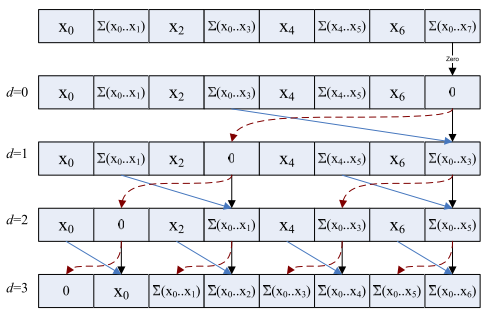
\includegraphics[width=0.8\textwidth]{stateofart/gpgpu/blelloch_downsweep}
\caption{Representation of the down-sweep phase of Blelloch's algorithm \cite{Harris2007}. \emph{d} is the level of the tree.}
\label{fig:scan down-sweep}
\end{figure}

The computational complexity of this algorithm is higher than that of its sequential counterpart.
The sequential version has a $O(n)$ computational complexity, since it only goes through the input array once and performs exactly $n$ additions.
Blelloch's algorithm, on the other hand, performs $n-1$ additions in the reduce phase and $n-1$  in the down-sweep phase, but still keeps the linear work complexity of the sequential version.
Since it is a parallel algorithm and the computation will be distributed across several processing units, its performance is significantly better.
It should be noted that, as described, the algorithm supports input arrays of a size that is a power of $2$.
However, \citet{Harris2007} explains how to overcome this limitation and also offers the description of an implementation for CUDA along with hardware specific optimizations, which presented a speed-up as high as 6.

% % % % % % % % % % % % % % % % % % % % % % % % % % % % % % % % % % % % % % % %
%
%  					QUANTUM CLUSTERING
%
% % % % % % % % % % % % % % % % % % % % % % % % % % % % % % % % % % % % % % % %

\section{Quantum clustering}
\label{sec:quantum clustering}

The field of quantum clustering has shown promising results regarding potential speed-ups in several tasks over their classical counterparts. 
Currently, two major approaches for the concept of quantum clustering were found in the literature: quantization of clustering methods to work in quantum computers or algorithms inspired by quantum physics.

The former approach translates in converting algorithms to work partially or totally on a different computing paradigm, with support of quantum circuits or quantum computers.
% relevant papers for machine learnigng quantum paradigm
Both \citet{Aimeur2013} and \citet{Lloyd2013} show how the quantum paradigm can be used for speed-ups in machine learning algorithms, with the possibility of obtaining exponential speed-ups.
Many of these quantizations make use of Groover's database search algorithm \cite{grover1996fast}, or a variant of it, e.g. \citet{Wiebe2014}.
Most literature on this approach is also mostly theoretical, since the physical requirements still do not exist for testing these methods.
This approach can be seen as part of the bigger problem of quantum computing and quantum information processing.
An alternative to using real quantum systems would be to simulate them.
% get refs for simulation of quantum systems not being feasable; Feynmann; I think washington course had something
However, simulating quantum systems in classical computers is a very hard task by itself and literature suggest that it is not feasible \cite{Feynman1982}.
% Given that the scope of the thesis is to accelerate clustering, having the extra overhead of simulating the systems would not allow speed-ups. 
The quantization approach falls outside the scope of this dissertation, but \citet{wittek2014quantum} offers a thorough review on the state of the art of machine learning in the quantum paradigm.

% Computational intelligence is the second approach, i.e. to use algorithms that muster inspiration from quantum analogies.
The second approach is part of the wider field of Computational Intelligence.
A study of the literature reveals that it typically further divides itself into two categories \cite{Casper2013}. 
One comprises the algorithms based on the concept of the qubit, the quantum analogue of a classical bit with interesting properties found in quantum objects.
Several algorithms have been modeled after this concept, often also gathering inspiration from evolutionary genetic algorithms, which were successfully applied in several areas:
\begin{itemize}
	\item tackling the Knapsack problem as described in \citet{Han2000} and its improved version \cite{Liu2010};

	\item solving the traveling salesman problem \cite{Talbi2004};

    \item two implementations of a Quantum K-Means algorithm \cite{Casper2012KMeans,Xiao2010};

    \item a Quantum Artificial Bee Colony algorithm \cite{hung2013quantum,Casper2013};

    \item two approaches for Fuzzy C-Means (FCM), namely Quantum New Weighted Fuzzy C-Means (QNW-FCM) \cite{Casper2013} and Quantum Fuzzy C-Means (QFCM) \cite{hung2013quantumcmeans,Casper2013};

    \item a novel quantum inspired clustering technique based on manifold distance \cite{Liang2009};

    \item a Quantum-inspired immune clonal clustering algorithm based on watershed \cite{Li2010}.
\end{itemize}

%schrodinger
The other approach models data as a quantum system and uses Schrödinger's equation in some way.
Often, the data is modeled as a quantum system, where each pattern is a particle, and Schrödinger's equation is used to evolve the particle system into a solution.
This has been applied in an optimization problem for electromagnetics using a quantum particle swarm \cite{mikki2006quantum} and also on several clustering algorithms:
\begin{itemize}
	\item the Quantum Clustering \cite{Horn2001b} algorithm treats patterns as quantum particles whose potential is computed with Schrödinger's equation and the system is evolved with the Gradient Descent method;

	\item Dynamic Quantum Clustering \cite{Weinstein2009} is a variation of \citet{Horn2001b} that uses Schrödinger's equation to evolve the system;

	\item a Fuzzy C-Means approach \cite{li2007quantum} based on Quantum Clustering \cite{Horn2001b};

	\item QPSO+FCM, a Fuzzy C-means \cite{Wang2007} based on Quantum-behaved Particle Swarm Optimization (QPSO) \cite{Sun2004}.

\end{itemize}

For more information on quantum inspired algorithms, the reader is referred to \citet{Manju2014} which offers a thorough survey on the state of the art of quantum inspired computation intelligence algorithms.
The following two sections contain a brief overview of the concept of the qubit and the description of an algorithm that uses this approach.
Afterwards, an algorithm that follows the Schrödinger's equation approach is reviewed.

\subsection{The quantum bit approach}
\label{sec:qubit}

\subsubsection{The quantum bit}

To understand the algorithms based on the concept of the qubit, it is useful to cast some insight about its properties and functioning.
This section has the purpose to provide a brief introduction to this topic.
An extended and in-depth review of this and related topics can be found in \citet{Lanzagorta2008}.
The qubit is a quantum object with certain quantum properties such as entanglement and superposition.
Within the context of the studied algorithm, the only property used is superposition.
A qubit can have any value between 0 and 1 (superposition property) until it is observed, which is when the system collapses to either state.
However, the probability with which the system collapses to either state  may be different.
The superposition property or linear combination of states can be expressed \cite{Casper2012KMeans} as % add ref for the mathematical formulation below: this can be found in the QK-Means papers


$$
% [\psi] = \alpha[0] + \beta[1]
| \psi \rangle = \alpha | 0 \rangle + \beta | 1 \rangle
$$

where $\psi$ is an arbitrary state vector and $\alpha$, $\beta$ are the the probability amplitude coefficients of basis states $| 0 \rangle$ and $| 1 \rangle$, respectively.
The Dirac bra ket notation is employed, where the \emph{ket} $| . \rangle$ corresponds to a column vector.
The basis states correspond to the spin of the modeled particle (in this case, a ferminion, e.g. electron).
The coefficients are subjected to the following normalization:

$$|\alpha|^2 + |\beta|^2 = 1$$

where $|\alpha|^2$, $|\beta|^2$ are the probabilities of observing states $[0]$ and $[1]$, respectively, and $\alpha$ and $\beta$ are complex quantities that represent a qubit:

$$\begin{bmatrix}
\alpha \\
\beta
\end{bmatrix}$$

Moreover, a qubit string may be represented by:
$$
\begin{bmatrix}
\left. \begin{matrix}
\alpha_1\\ 
\beta_1
\end{matrix}\right| & \left.\begin{matrix}
\alpha_2\\ 
\beta_2
\end{matrix}\right| & \begin{matrix}
\alpha_3\\ 
\beta_3
\end{matrix}
\end{bmatrix}
$$

The probability of observing the state $|000 \rangle$ will be $|\alpha_1|^2 \times |\alpha_2|^2 \times |\alpha_3|^2$.
To use this model for computing purposes, black-box objects called \emph{oracles} are used.
Oracles are important to understand quantum speed-ups.
They can be understood as subroutines that cannot be usefully examined or as unknown physical systems that perform a quantum operation on a qubit string \cite{Rosenbaum2011} and with properties one would like to estimate.
Within the context of the present work an oracle is an abstraction for the programmer.
It is an object which can be called and changes state (which can be observed) as a consequence.
For the purpose of the following sections, the concept of the oracle is more related to \emph{oracles with internal randomness} \cite{Rosenbaum2011} or, more simply, a probabilistic Turing machine, as in the case of \cite{hung2013quantum}.

% # get ref -->
% Def from wiki: In complexity theory and computability theory, an oracle machine is an abstract machine used to study decision problems.
% It can be visualized as a Turing machine with a black box, called an oracle, which is able to decide certain decision problems in a single operation.
% The problem can be of any complexity class.
% Even undecidable problems, like the halting problem, can be used. %from http://en.wikipedia.org/wiki/Oracle_machine


\subsubsection{Quantum K-Means}
\label{sec:qkmeans}

% Several clustering algorithms \cite{Casper2013,Casper,Xiao2010}, as well as optimization problems \cite{Wang2013}, are modeled after this concept.
% To test the potential of the algorithms under this paradigm, a quantum variant of the K-Means algorithm based on\cite{Casper} was chosen as a case study.

% This section will describe the Quantum K-Means algorithm \cite{Casper2012KMeans}.


% \subsubsection{Description of the algorithm}

The Quantum K-Means (QK-Means) algorithm, as described in \cite{Casper2012KMeans}, is based on the classical K-Means algorithm.
It extends the basic K-Means with concepts from quantum mechanics (the qubit) and evolutionary genetic algorithms.

Within the context of this algorithm, oracles contain strings of qubits and generate their own input by observing the state of the qubits.
After collapsing, the qubit value corresponds to a classical bit, with a binary value.

Ideally, oracles would contain actual quantum systems or simulate them - this would correctly account for the desirable quantum properties.
As it stands, oracles are not quantum systems or even simulate them and can be more appropriately described as random number generators.
Each string of qubits represents a number, so the number of qubits in each string will define its precision.
The number of strings chosen for the oracles depends on the number of clusters and dimensionality of the problem (e.g. for 3 centroids of 2 dimensions, 6 strings will be used since 6 numbers are required).
Each oracle will represent a possible solution.

The algorithm has the following steps:
\begin{enumerate}
\item Initialize population of oracles
\item Collapse oracles
\item K-Means
\item Compute cluster fitness
\item Store
\item Quantum Rotation Gate
\item Collapse oracles
\item Quantum cross-over and mutation
\item Repeat 3-7 until generation (iteration) limit is reached
\end{enumerate}


\paragraph{Initialize population of oracles}

The oracles are created in this step and all qubit coefficients are initialized with $\frac{1}{\sqrt{2}}$, so that the system will observe either state of the qubit with equal probability.
This value is chosen taken into account the necessary normalization of the coefficients, as described in the previous section.

\paragraph{Collapse oracles}

Collapsing the oracles implies making an observation of every qubit of each string in all oracles.
This is done by first choosing a coefficient to use (either can be used), e.g. $\alpha$.
Then, a random value $r$ between 0 and 1 is generated.
If $\alpha \ge r$ then the system collapses to $[0]$, otherwise to $[1]$.

\paragraph{K-Means}
In this step we convert the binary representation of the qubit strings to base 10 and use those values as initial centroids for K-Means.
For each oracle, classical K-Means is then executed until it stabilizes or reaches the iteration limit.
The solution centroids are returned to the oracles in binary representation.

\paragraph{Compute cluster fitness}
Cluster fitness is computed using the Davies-Bouldin index for each oracle.
The score of each oracle is stored in the oracle itself.

\paragraph{Store}
The best scoring oracle is stored.

\paragraph{Quantum Rotation Gate}
So far, the algorithm consisted of the classical K-Means with a complex random number generation for the centroids and complicated data structures, namely the oracles.
This is the step that fundamentally differs from the classical version.
In this step, a quantum gate (in this case a rotation gate) is applied to all oracles except the best one.
The basic idea is to shift the qubit coefficients of the least scoring oracles in the direction of the best scoring one.
These oracles will have a higher probability of collapsing into initial centroid values closer to the best solution so far.
This way, in future generations, the oracles do not initiate with the best centroids so far (which would not converge into a better solution) but we they are close while still ensuring diversity (which is also a desired property in the genetic computing paradigm).
In other words, we look for better solutions than the one we got before in each oracle while moving in the direction of the best we found so far.

The genetic operations of cross-over and mutation are both part of the genetic algorithms toolbox.
Literature suggests that this operations may not be required to produce variability in the population of qubit strings \cite{Liu2010}.
The reason for this is that enough variability is produced with the use of the angle-distance rotation method \cite{Liu2010} in the quantum rotation operation, with a careful choice of the rotation angle.
Still, when used, the goal of these operations is to produce further variability into the population of qubit strings.

\subsection{Schrödinger's equation approach} % Horn and Gottlieb's algorithm}
\label{sec:horn}

The other approach to clustering that gathers inspiration from quantum mechanical concepts is to use the Schrödinger equation.
The algorithm under study was created by Horn and Gottlieb \cite{Horn2010} and was later extended by Weinstein and Horn \cite{Weinstein2009}.

The first step in this methodology is to compute a probability density function of the input data.
This is done with a Parzen-window estimator in \cite{Horn2001a,Weinstein2009}.
The Parzen-window density estimation of the input data is done by associating a Gaussian with each point, such that

$$ \psi (\mathbf{x}) = \sum ^N _{i=1} e^{- \frac{\left \| \mathbf{x}-\mathbf{x}_i \right \| ^2}{2 \sigma ^2}} $$

where $N$ is the total number of points in the dataset, $\sigma$ is the variance and $\psi$ is the probability density estimation. $\psi$ is chosen to be the wave function in Schrödinger's equation.
%The details of why this is fall outside of the scope of the present work and are explained in \cite{Weinstein2009,Horn2001a,Horn2001b}.
Further details can be found in \citet{Weinstein2009,Horn2001a,Horn2001b}.

With this information, one will compute the potential function $V(x)$ that corresponds to the state of minimum energy (ground state = eigenstate with minimum eigenvalue) \cite{Horn2001a}, by solving the Schrödinger's equation in order of $V(x)$:      

\begin{align}
V \left ( \mathbf{x} \right ) = E + \frac {\frac{\sigma^2}{2}\nabla^2 \psi }{\psi}
= E - \frac{d}{2} + \frac {1}{2 \sigma^2 \psi} \sum ^N _{i=1} \left \| \mathbf{x}-\mathbf{x}_i \right \| ^2 e^{- \frac{\left \| \mathbf{x}-\mathbf{x}_i \right \| ^2}{2 \sigma ^2}}
\label{eq:wave}
\end{align}

And since the energy should be chosen such that $\psi$ is the groundstate (i.e. eigenstate corresponding to minimum eigenvalue) of the Hamiltonian operator associated with Schrödinger's equation (not represented above), the following is true

\begin{align}
E = - min \frac {\frac{\sigma^2}{2}\nabla^2 \psi }{\psi}
\label{eq:wave sol}
\end{align}

From equations \ref{eq:wave} and \ref{eq:wave sol}, $V(x)$ can be computed.
This potential function is related to the inverse of a probability density function.
Minima of the potential correspond to intervals in space where points are together.
So minima will naturally correspond to cluster centers \cite{Horn2001a}.
However, it is very computationally intensive to compute $V(x)$ to the whole space, so the compututation of the potential function is only done at the data points.
This should not be problematic since clusters' centers are generally close to the data points themselves. 
Even so, the minima may not lie on the data points themselves.
One method to address this problem is to compute the potential on the input data and converge these points toward some minima of the potential function.
This is done with the gradient descent method in \cite{Horn2001a}. 

Another method \cite{Weinstein2009} is to think of the input data as particles and use the Hamiltonian operator to evolve the quantum system in the time-dependent Schrödinger's equation.
Given enough time steps, the particles will converge to and oscillate around potential minima.
This method makes the Dynamic Quantum Clustering algorithm.
The nature of the computations involved in this algorithm make it a good candidate for parallelization techniques.
\citet{Wittek2013} parallelized this algorithm to the GPU obtaining speed-ups of up to two magnitudes relative to an optimized multicore CPU implementation. %TODO: leave this or not? I did not test this so maybe it is better not

% #TODO describe the fine cluster algorithm; critique how this is done; what was developed;

%[1] N. Wiebe, A. Kapoor, and K. Svore, “Quantum Algorithms for Nearest-Neighbor Methods for Supervised and Unsupervised Learning,” p. 31, 2014.
%
%\cite{Wiebe2014}

%[2] D. Horn and A. Gottlieb, “The Method of Quantum Clustering.,” NIPS, no. 1, 2001.
%\cite{Horn2001a}

%[3] M. Weinstein and D. Horn, “Dynamic quantum clustering: a method for visual exploration of structures in data,” Phys. Rev. E - Stat. Nonlinear, Soft Matter Phys., vol. 80, no. 6, pp. 1–15, Dec. 2009.
%\cite{Weinstein2009}

%[4] E. Casper and C. Hung, “Quantum Modeled Clustering Algorithms for Image Segmentation,” vol. 2, no. March, pp. 1–21, 2013.
%\cite{Casper2013}
%
%[5] E. Casper, C.-C. Hung, E. Jung, and M. Yang, “A Quantum-Modeled K-Means Clustering Algorithm for Multi-band Image Segmentation.” [Online]. Available: http://delivery.acm.org/10.1145/2410000/2401639/p158-casper.pdf?ip=193.136.132.10&id=2401639&acc=ACTIVE SERVICE&key=2E5699D25B4FE09E.F7A57B2C5B227641.4D4702B0C3E38B35.4D4702B0C3E38B35&CFID=476955365&CFTOKEN=55494231&__acm__=1423057410_0d77d9b5028cb3. [Accessed: 04-Feb-2015].

%\cite{Casper}

%[6] J. Xiao, Y. Yan, J. Zhang, and Y. Tang, “A quantum-inspired genetic algorithm for k-means clustering,” Expert Syst. Appl., vol. 37, pp. 4966–4973, 2010.
%\cite{Xiao2010}

%
%[7] H. Wang, J. Liu, J. Zhi, and C. Fu, “The Improvement of Quantum Genetic Algorithm and Its Application on Function Optimization,” vol. 2013, no. 1, 2013.
%\cite{Wang2013}

%
%[8] W. Liu, H. Chen, Q. Yan, Z. Liu, J. Xu, and Y. Zheng, “A novel quantum-inspired evolutionary algorithm based on variable angle-distance rotation,” 2010 IEEE World Congr. Comput. Intell. WCCI 2010 - 2010 IEEE Congr. Evol. Comput. CEC 2010, 2010.
%\cite{Liu2010} % add new .tex files for new chapters
%!TEX root = Thesis.tex

\chapter{EAC for large datasets: proposed solutions}
\label{chapter:methodology}


%TODO explain methodology to obtain results of quantum clustering of just present results on why it was not viable?

%TODO This is where I explain my approach to the problem of EAC in Big Data

The aim of this thesis is the optimization and scalability of EAC, with a focus for large datasets.
EAC is divided in three steps and each has to be considered for optimization.
This chapter will present the considered solutions for each step, which are also visually summarized in Fig. \ref{fig:proposed solutions}.

\begin{figure}[hbt!]
    \centering
    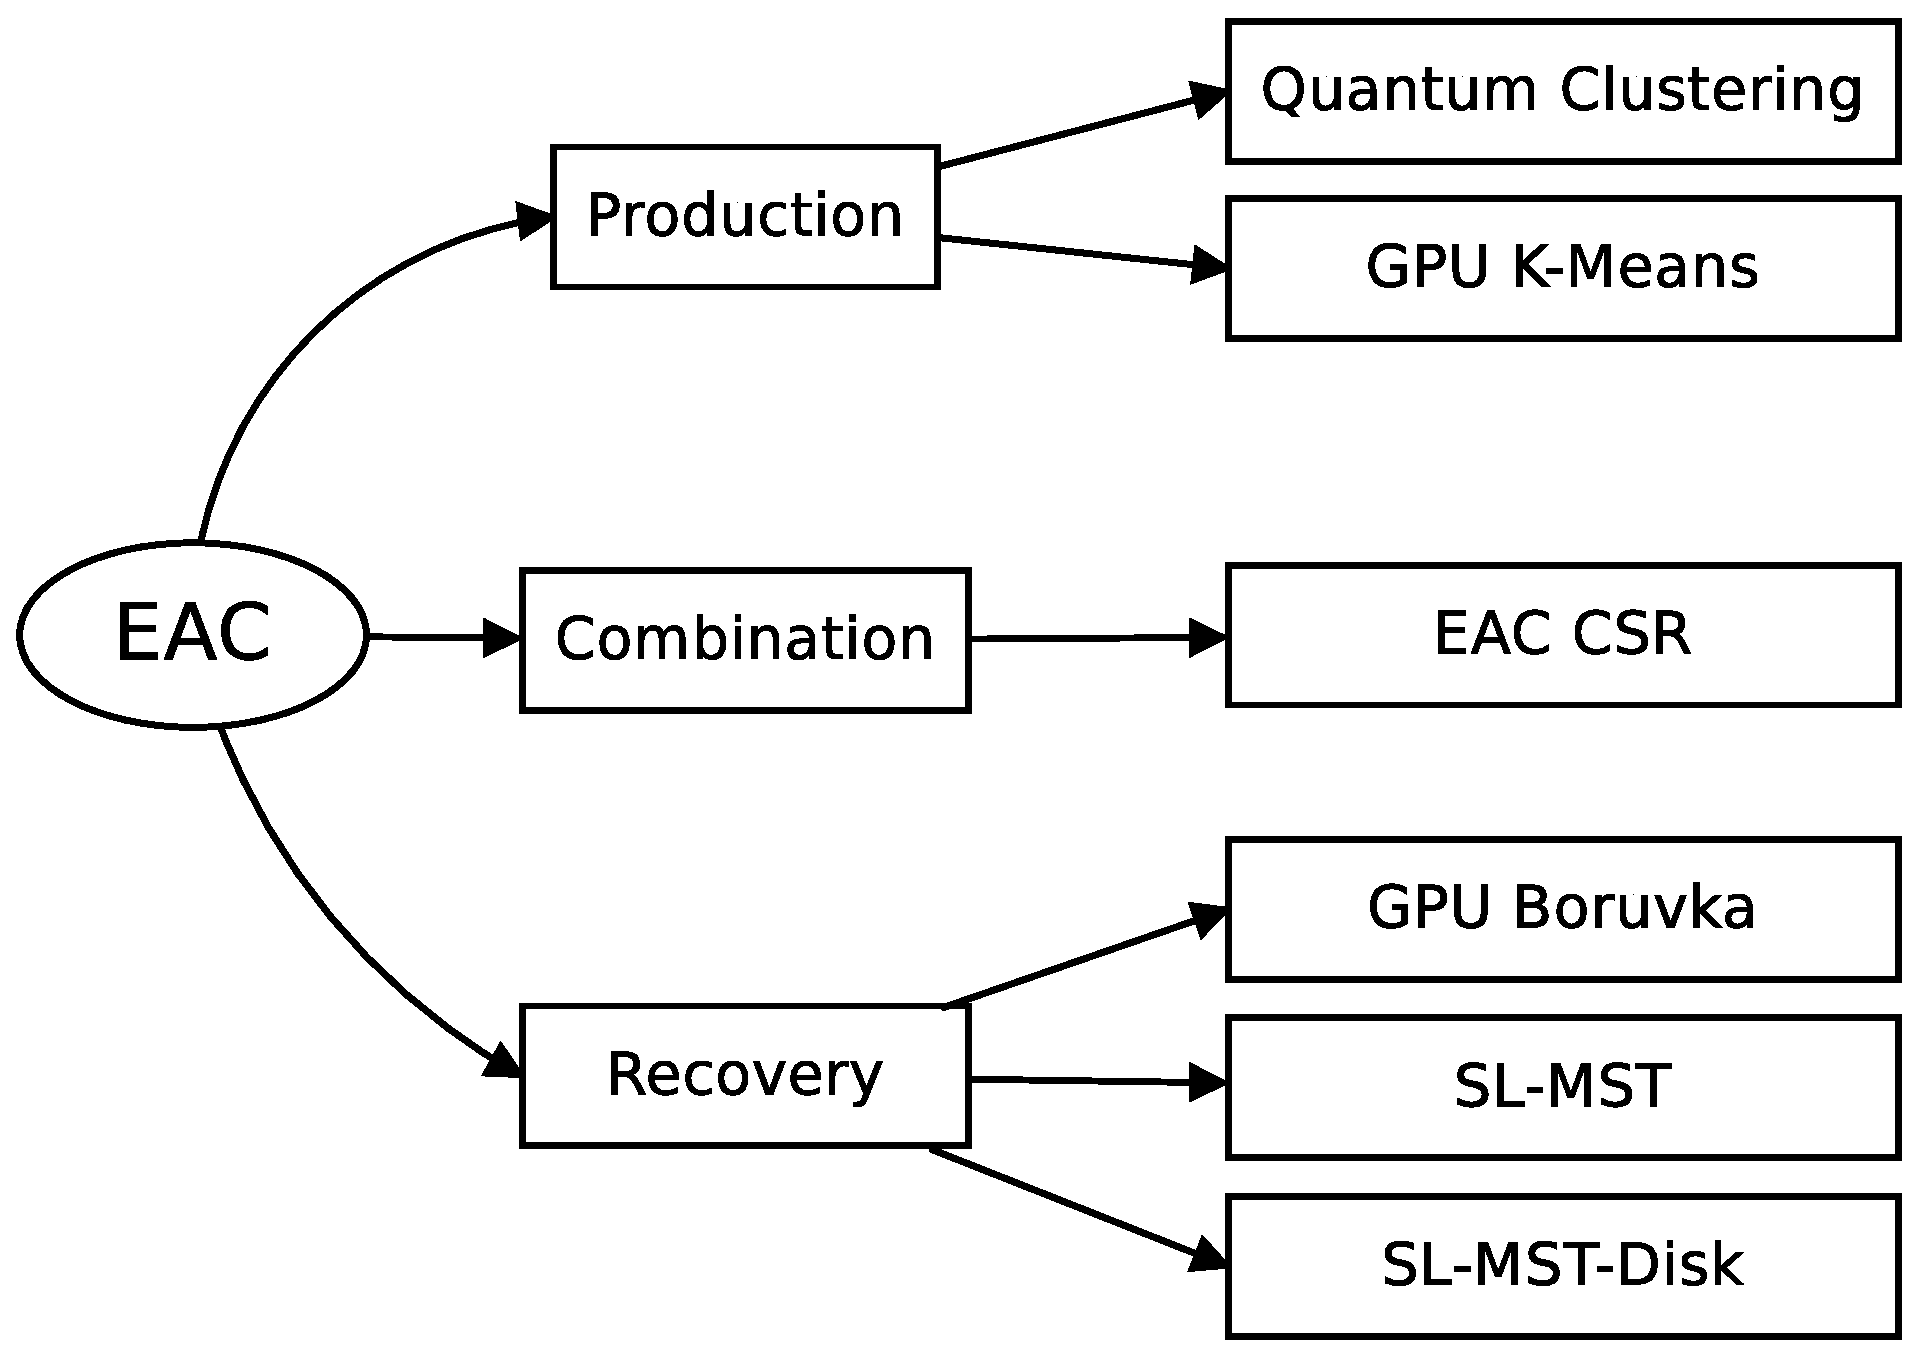
\includegraphics[width=0.6\textwidth]{{{methodology/diagram_proposed_solutions}}}
    \caption{Diagram of proposed solution in each phase of EAC.}
    \label{fig:proposed solutions}
\end{figure}

The first step is the gathering of evidence, i.e. generating an ensemble of partitions.
The main objective for the optimization of this step is speed.
Using fast clustering methods for generating partitions is an obvious solution, as is the optimization of particular algorithms aiming for the same objective.
Since each partition is independent from every other partition, parallel computing over a cluster of computing units would result in a fast ensemble generation.
Using either or any combination of these strategies will guarantee a speed-up.

Initial research was under the field of quantum clustering.
After this pursuit proved fruitless for being slow, the focus of research shifted to parallel computing, more specifically a K-Means parallel version within the GPGPU paradigm.
%After this pursuit proved fruitless regarding one of the main requirements (speed), the focus of research shifted to parallel computing, more specifically a K-Means parallel version within the GPGPU paradigm.
	
The second step is mostly bound by memory.
The complete co-association matrix has a space complexity of $\mathcal{O}(n^2)$.
Such complexity becomes prohibitive for big data, e.g. a dataset of $2 \times 10^6$ patterns will result in a complete co-association matrix of $14901 \; GB$ if values are stored in single precision floating-point format.
%This work was focused on sparse matrices.% and cutting associations.
This problem is addressed by exploring the inherent sparse nature of the co-association matrix.

The last step has to take into account both memory and speed requirements.
The final clustering must be able to produce good results and be fast while not exploding the already big space complexity from the co-association matrix.
The work in this last step was initially directed towards parallelization and afterwards out-of-core processing using a disk stored co-association matrix.% and sparse matrices.

The methodology for optimizing for speed is relevant and permeates the approach taken to every problem faced in the present work.
For optimizing the speed of an algorithm, one starts by first profiling that algorithm and analyze which parts take the longest to compute.
These parts are the focus of optimization as any change on them will have the greatest effect on the overall algorithm.
To further illustrate this point, let us consider an algorithm that spends 75\% of its time on a section of the code to which a speed-up of $2$ is possible and 25\% on a part to which an infinite speed-up is possible (this translates in its execution time being negligible).
Let us further assume that only one part of the algorithm may be optimized.
If one optimizes the first part, the local speed-up is $2$ and the overall speed-up is $1.6$.
On the other hand, if one optimizes the second part, the local speed-up is infinite but the overall speed-up is only $1.333(3)$.
%refer Amdhal Law? it is formally more oriented torwards parallel computing and number of threads

All the algorithms were implemented in Python with high reliance on numerical and scientific modules, namely NumPy \cite{VanDerWalt2011} and SciPy \cite{JonesSciPy,Oliphant2007,Millman2011}.
The main reason for using Python on all implementations was to use the same technology everywhere and have a high interoperability between modules.
Important modules for visualizing and processing statistical results were MatplotLib \cite{hunter2007matplotlib} and Pandas \cite{McKinney2010}, respectively.
The SciKit-Learn \cite{Pedregosa2011} machine learning library has a plethora of implemented algorithms which were used for benchmarking as well as integration in the devised solutions.
The iPython \cite{Perez2007} module was used for interactive computing which allowed for accelerated prototyping and testing of algorithms.
Python is an interpreted language which translates in its performance being worse than a compiled language such as C or Java.
To address this problem, the open-source Numba \cite{numba} module from Continuum Analytics was used to allow for writing code in native Python and have it converted to fast compiled code.
Furthermore, this module provides a pure Python interface for the CUDA API.
The proprietary NumbaPro module was used for two high level CUDA functions, namely \emph{argsort} and \emph{max}. %TODO write this one a bit better


\section{Quantum Clustering}

Research under this paradigm aimed to find a candidate for the first phase of EAC.
Two candidates were considered: Quantum K-Means (QK-Means) and Horn and Gottlieb's quantum clustering (QC) algorithm.
These algorithms were chosen so as to have a representative from both approaches of quantum inspired algorithms identified in chapter \ref{chapter:stateofart}.


The implementation of QK-Means followed the description presented in section \ref{sec:qkmeans}, with the exception of the removal of the genetic operations \emph{cross-over} and \emph{mutation}.
The main goal for the first phase of EAC is speed but these operations aim at improving the quality of the solution by producing variability in the oracles.
Furthermore, literature \cite{Liu2010} suggests that enough variability is produced in the quantum rotation step with the angle-distance rotation method.
As such, it was an implementation decision to cut the overhead of these operations for the sake of time optimization.

An implementation of QC was already available in Matlab.
Accordingly, implementing this algorithm translated into porting the code from Matlab to Python.

% For both, the experiments that were setup had the goal of evaluating the speed and accuracy performances of the algorithms.


% This should be 
% Under the qubit concept, no other algorithms were experimented with since the results for this particular algorithm showed that this kind of approach is infeasible due to the cost in computational speed.
% The results highlight that fact.

\section{Speeding up Ensemble Generation with Parallel K-Means}

K-Means is an obvious candidate for the generation of partitions since it is simple, fast and partitions do not need to be accurate - variability in the partitions is a desirable property.
This relaxation on the accuracy of the partitions already allows for a faster generation of partitions since fewer iterations of the algorithm need to be executed for a partition to be generated - typically 3 iterations suffice.
Further gains are possible with a parallel GPU version of K-Means.
The overview of the algorithm used is presented in section \ref{sec:art parallel kmeans}, but some implementation differences exist, namely the lack of some optimizations used in the original source.
The choice to only parallelize the labeling phase was motivated by the maximum potential speed-ups presented below.
Afterwards, the implementation is described.

\subsection{Maximum potential speed-up}

Previously, it was mentioned that the methodology followed for speeding up an application was to first profile the code and identify the portions of code that can be optimized and what fraction of the total computational time they take.
Table \ref{tab:kmeans max speedup} presents statistical results on the theoretical maximum speed-up for the two K-Means phases.
These results came from the same experiment as that presented in section \ref{sec:parallel kmeans}.
The sequential version of K-Means was executed over a wide spectrum of datasets varying the number of patterns, dimensions and centroids.
The theoretical maximum speed-up is considered to be the overall speed-up of the algorithm if one of its phases had infinite speed-up, i.e. when its time is negligible relative to the other phases.
Analyzing these results it is clear that the labeling phase holds the most potential for optimizations.
Furthermore, the theoretical speed-up also increases with the problem complexity (number of patterns, dimensions and centroids), since, the execution time for the labeling phase with more complex datasets is higher compared to the update phase.
The theoretical speed-up of the update phase is almost negligible when compared to the labeling phase.
This illustrates the importance of profiling the code before proceeding with optimizations, since effort invested in the update phase would yield little effect.

\begin{table}[h]
\centering
\caption{Maximum theoretical speed-up for the labeling and update phases of K-Means based on experimental data. The datasets used range from $1000$ to $500 \: 000$ patterns, from $2$ to $1000$ dimensions and from $2$ to $2048$ centroids.}

\begin{tabular}{lrr}
\toprule
{} &  Labeling phase &  Update phase \\
\midrule
mean  &               540.8308 &                    1.0468 \\
std   &               879.9143 &                    0.0836 \\
min   &                 2.9983 &                    1.0002 \\
25\% percentile &      18.6578 &                    1.0015 \\
50\% percentile &      99.8681 &                    1.0101 \\
75\% percentile &     681.2509 &                    1.0567 \\
max   &              5026.9722 &                    1.5199 \\
\bottomrule
\end{tabular}

\label{tab:kmeans max speedup}
\end{table}

\subsection{Implementation details}

The implementation gives as much freedom as possible to the user regarding CUDA parameter choices, such as the threads per block, blocks per grid or number of patterns to process per thread.
By default, each thread will compute the label of one pattern and the blocks are unidimensional and composed by 512 threads, which maximizes GPU occupancy since no shared memory is used.
The number of blocks, then, is the number of patterns divided by the number of threads per block.
If the number of blocks exceeds the maximum allowed for one dimension (65535), the grid configuration automatically uses other dimensions.
The other parameter that the user can choose deals with how data is transfered back and forward between host and device.
The user can choose to allow the Numba CUDA API to handle all the memory transfers or to allow the implementation to optimize those.
The latter will minimize the amount of data transfers and memory allocations and is the default option.
Furthermore, it also allows for the algorithm to be executed multiple times without redundant transfer of the pattern set.
This permits the production of an entire ensemble with a single transfer of the pattern set.
These parameters (number of patterns per thread, number of threads per block and memory transfer mode) may be configured at runtime.
Still, a typical user does not need to be knowledgeable about CUDA to be able to use this implementation, since the tuning of these parameters is optional.

The CUDA implementation of the label computation part of the algorithm starts by transferring the data to global memory (pattern set and initial centroids) and allocates space for the labels and corresponding distances, also in global memory.
Both data and centroids are transfered and stored in a row-major order and all memory transfers are synchronous.
The computation of a label for one pattern is done by iteratively computing the distance from the pattern to each centroid and storing the label and the distance corresponding to the closest centroid.
Finally, the labels and distances are sent back to the host for computation of the centroids.
This procedure is available as a CUDA kernel or as three different sequential versions: pure Python, based on NumPy or compiled code with Numba.
These same sequential versions exist for the recomputation of the centroids.
The fastest of CPU versions is the Numba based, followed by the one based on NumPy and finally pure Python.
The implementation of the centroid computation starts by counting the number of patterns attributed to each centroid.
Afterwards, it checks if there are any "empty" clusters, i.e. if there are centroids that are not the closest ones to any pattern.
Dealing with empty clusters is important because, although empty clusters may be desirable in some situations, the target use expects that the output number of clusters to be the same as defined in the input parameter.
Centroids corresponding to empty clusters will be the patterns that are furthest away from their centroids, which is the reason why the distances to the centroids are kept and transfered.
Any other centroid $c_i$ will be the mean of the patterns that were labeled $i$.

At the end of each iteration, a stopping criteria is checked: either the difference between the centroids of two consecutive iterations reached an user supplied threshold (default of 0.0001) or the maximum number of iterations was reached (default of 300).
In EAC, the number of iterations is the stopping criteria used with a low number of iterations (e.g. 3 in the present work).


\section{Dealing with the space complexity of the co-association matrix}

In chapter \ref{chapter:stateofart}, two approaches to the space complexity of the co-association matrix in the second phase of EAC are presented: one dealing with $p$ prototypes and the other with the inherent sparsity of the matrix. 

The results presented in the sparsity study of EAC \cite{Lourenco2010} show that it is possible to obtain a high sparsity in the co-association matrix.
In some cases the density of the matrix was as low as 1\%.
This motivated the focus of the work on exploiting the inherent sparsity of the matrix.
A discussion on using sparse matrices and a novel solution for building the co-association matrix is presented in section \ref{sec:sparse coassoc}.

As stated before, the focus of the work is on sparse matrices.
Still, for the sake of completeness, the different strategies considered for the prototypes approach are discussed here.
One strategy is to use the \textbf{p-Nearest Neighbors} as prototypes, as already presented in chapter \ref{chapter:stateofart}.
Before building the co-association matrix, the $p$ closest patterns to each pattern are computed and stored in the $n \times p$ neighbor matrix.
During the voting mechanism of EAC only the neighbors of each pattern are considered.
This strategy has a space complexity of $O(2nk)$ and requires the computation of the k-Nearest Neighbors.
A second strategy is to use \textbf{p random prototypes}, which will be a set of unique $p$ patterns.
This will be the same for every pattern.
Here the voting mechanism is altered so that if a pattern is clustered with any of the prototypes, the correspondent element in the co-association matrix is incremented.
This has the advantage that only a $n \times p$ matrix needs to be stored along with a $p$ array for the chosen prototypes.
Furthermore, if $p$ is high enough to provide a representative pattern of the dataset the results can be as good as the full matrix.
The third, and final, possible strategy identified is similar to the random prototypes.
The difference is that instead of choosing $p$ random patterns from the dataset, the prototypes will be the representatives of the dataset from another algorithm, e.g. K-Medoids, K-Means.

It would be ideal to combine both approaches (sparsity and neighbors) to further reduce space complexity, but they are not necessarily compatible.
This is specially true for the p-Nearest Neighbors strategy since it is unlikely that a pattern will never be clustered with its closest $p$ neighbors.
This means that the $n \times p$ co-association matrix may not have many zeros which translates in little advantage for using the sparsity augmentation approach the matrix of co-associations.
% Still, one should note that the p-Nearest Neighbors strategy is closely related to a sparse representation.
% these seem more like comments for results.
% Still, this highly depends on the number of neighbors relative to the number of patterns and also the granularity of the partitions.
% If the number of neighbors is high, one of the neighbors can be sufficiently far away from the pattern to not clustered with it.
% If the granularity of the partitions is high (i.e. there are a high number of small clusters) then each cluster may have sufficiently few patterns that neighbors are not included.

\section{Building the sparse matrix}
\label{sec:sparse coassoc}

Building a non-sparse matrix is easy and fast since the memory for the whole matrix is allocated and indexing the matrix is direct.
When using sparse matrices, neither is true.
In the specific case of EAC, there is no way to know what is the number of associations the co-association matrix will have which means it is not possible to pre-allocate the memory to the correct size of the matrix.
This translates in allocating the memory gradually which may result in fragmentation, depending on the implementation, and more complex data structures, which incurs overhead.

% Several sparse matrices exist
% some are better for building others for computing
% describe my solution

Documentation of the SciPy library recommends different sparse formats for either building a matrix or operating over it.
For building a matrix, the COO (COOrdinate), DOK (Dictionary of Keys) and LIL (List of Lists) formats are recommended.
All of these formats rely on extra data structures such as lists as dictionaries to efficiently build the matrices incrementally, i.e. allocating memory as it is required.
For operating over a matrix, the documentation recommends converting from one of the previous formats to either CSR (Compressed Sparse Row) or CSC (Compressed Sparse Column).

%TODO insert real times from small simulation
As observed before, the sparsity study of EAC \cite{Lourenco2010} did not account for the overhead of using the data structures supporting sparse matrices.
However, scaling to very large datasets must take this into account.
Exploratory testing revealed that using one of the recommended matrices, allowed for building the matrix took around two orders of magnitude as long as using a full allocated matrix.
Furthermore, because of the extra data structures, the implementations from SciPy would saturate the main memory from datasets with less than 1 million patterns.
Using the CSR format did not saturate memory but it took a completely unacceptable amount of time, many orders of magnitude above any of the formats recommended for building the matrix.

After a search in the literature for efficient and scalable ways to build a sparse matrix proved fruitless, these problems motivated the design of a new method for building the matrix specialized for the characteristics of EAC.
The solution devised is based on the CSR format (described previously in section \ref{sec:parallel_SL}), which has the desired properties of having a low memory trace and allows for fast computations.

\subsection{EAC CSR}

The first step is making an initial assumption on the maximum number of associations \emph{max\_assocs} that each pattern can have.
A possible rule is $$max\_assocs = 3 \times bgs$$ where $bgs$ is the biggest cluster size in the ensemble.
The biggest cluster size is a good heuristic for trying to predict the number of associations a pattern will have since it is the limit of how many associations each pattern will have in any partition.
Furthermore, one would expect that the neighbors of each pattern will not vary significantly, i.e. the same neighbors will be clustered together with a pattern repeatedly in many partitions.
This rule was motivated by the relationship between the maximum number of associations and the biggest cluster size, which will be presented in the results.
This scheme for building the matrix uses 4 supporting arrays, 3 of which (\emph{indices}, \emph{data} and \emph{indptr}) are part of the standard CSR format. The arrays are:

\begin{itemize}
	\item \textbf{indices} - an array of $n \times max\_assocs$ size that stores the columns of each non-zero value of the matrix, i.e. the destination pattern to which each pattern associates with;
	\item \textbf{data} - an array of $n \times max\_assocs$ size that stores all the non-zero values;
	\item \textbf{indptr} - an array of $n$ size where the \emph{i-th} element is the index of the \emph{indices} and \emph{data} arrays that holds the value and column of the first non-zero value in the \emph{i-th} row.
	\item \textbf{degree} - an array of $n$ size that stores the number of non-zero values of each row.
\end{itemize}

Each pattern (row) has a maximum of \emph{max\_assocs} pre-allocated that it can use to fill with new associations.
New associations that exceed this pre-allocated maximum are discarded.
%Since each pattern has a maximum pre-defined number of associations, \emph{indptr} does not really need to exist since it can be easily deduced (e.g. $indices[n] = n \times max\_assocs$).
The \emph{degree} array is the one keeping track of the number of associations of each pattern.
The data types used are picked to be smallest necessary for the problem at hand.
The \emph{data} array is usually composed of singly Byte unsigned integer values since the ensemble size is typically less than 255.
The \emph{indices} array stores unsigned integers of the smallest size possible to store the number of patterns of the dataset.
The data type of \emph{indptr} is an 8 Byte integer, since the number of associations of large problems are usually often bigger than $2^{32}$.
Lastly, the \emph{degree} array stores 4 Byte unsigned integers.
The last two data types never change, since the size of the \emph{indptr} and \emph{degree} arrays is usually negligible compared to the combined size of the \emph{data} and \emph{indices} arrays.
Throughout this section, the interval of the \emph{indices} array corresponding to a specific pattern (row) is referred to as that pattern's \emph{indices} interval.
If it is said that an association is added to the end of the \emph{indices} interval, this refers to the beginning of the part of the interval that is free for new associations.
The term indices is used either in the context of the array, in which case it will appear as \emph{indices}, or as the plural of index, in which case it will appear as indices.
Furthermore, it should be noted that this method assumes that the clusters received come sorted in a increasing order.

The first partition is inserted in a special way.
Since it is the first and the clusters are sorted, it is a matter of copying the cluster to the \emph{indices} array in the positions of each pattern, with the exclusion of the pattern itself.
The data array (containing the co-association score) is set to 1 on the relevant positions.
This process can be observed clearly in Fig. \ref{fig:first part}.
Because it is the fastest partition to be inserted, it is picked to be the one with the least amount of clusters (more patterns per cluster) so that each pattern gets the most amount of associations in the beginning (on average).
This is only applicable if the whole ensemble is provided, otherwise there is no way to know what is the biggest cluster of the whole ensemble.
This increases the probability that any new cluster will have more patterns that correspond to already established associations.
Because the clusters are sorted and only a copy of each cluster was made, it is not necessary to sort each row of the matrix by column index.

\begin{figure}[hbtp]
\centering
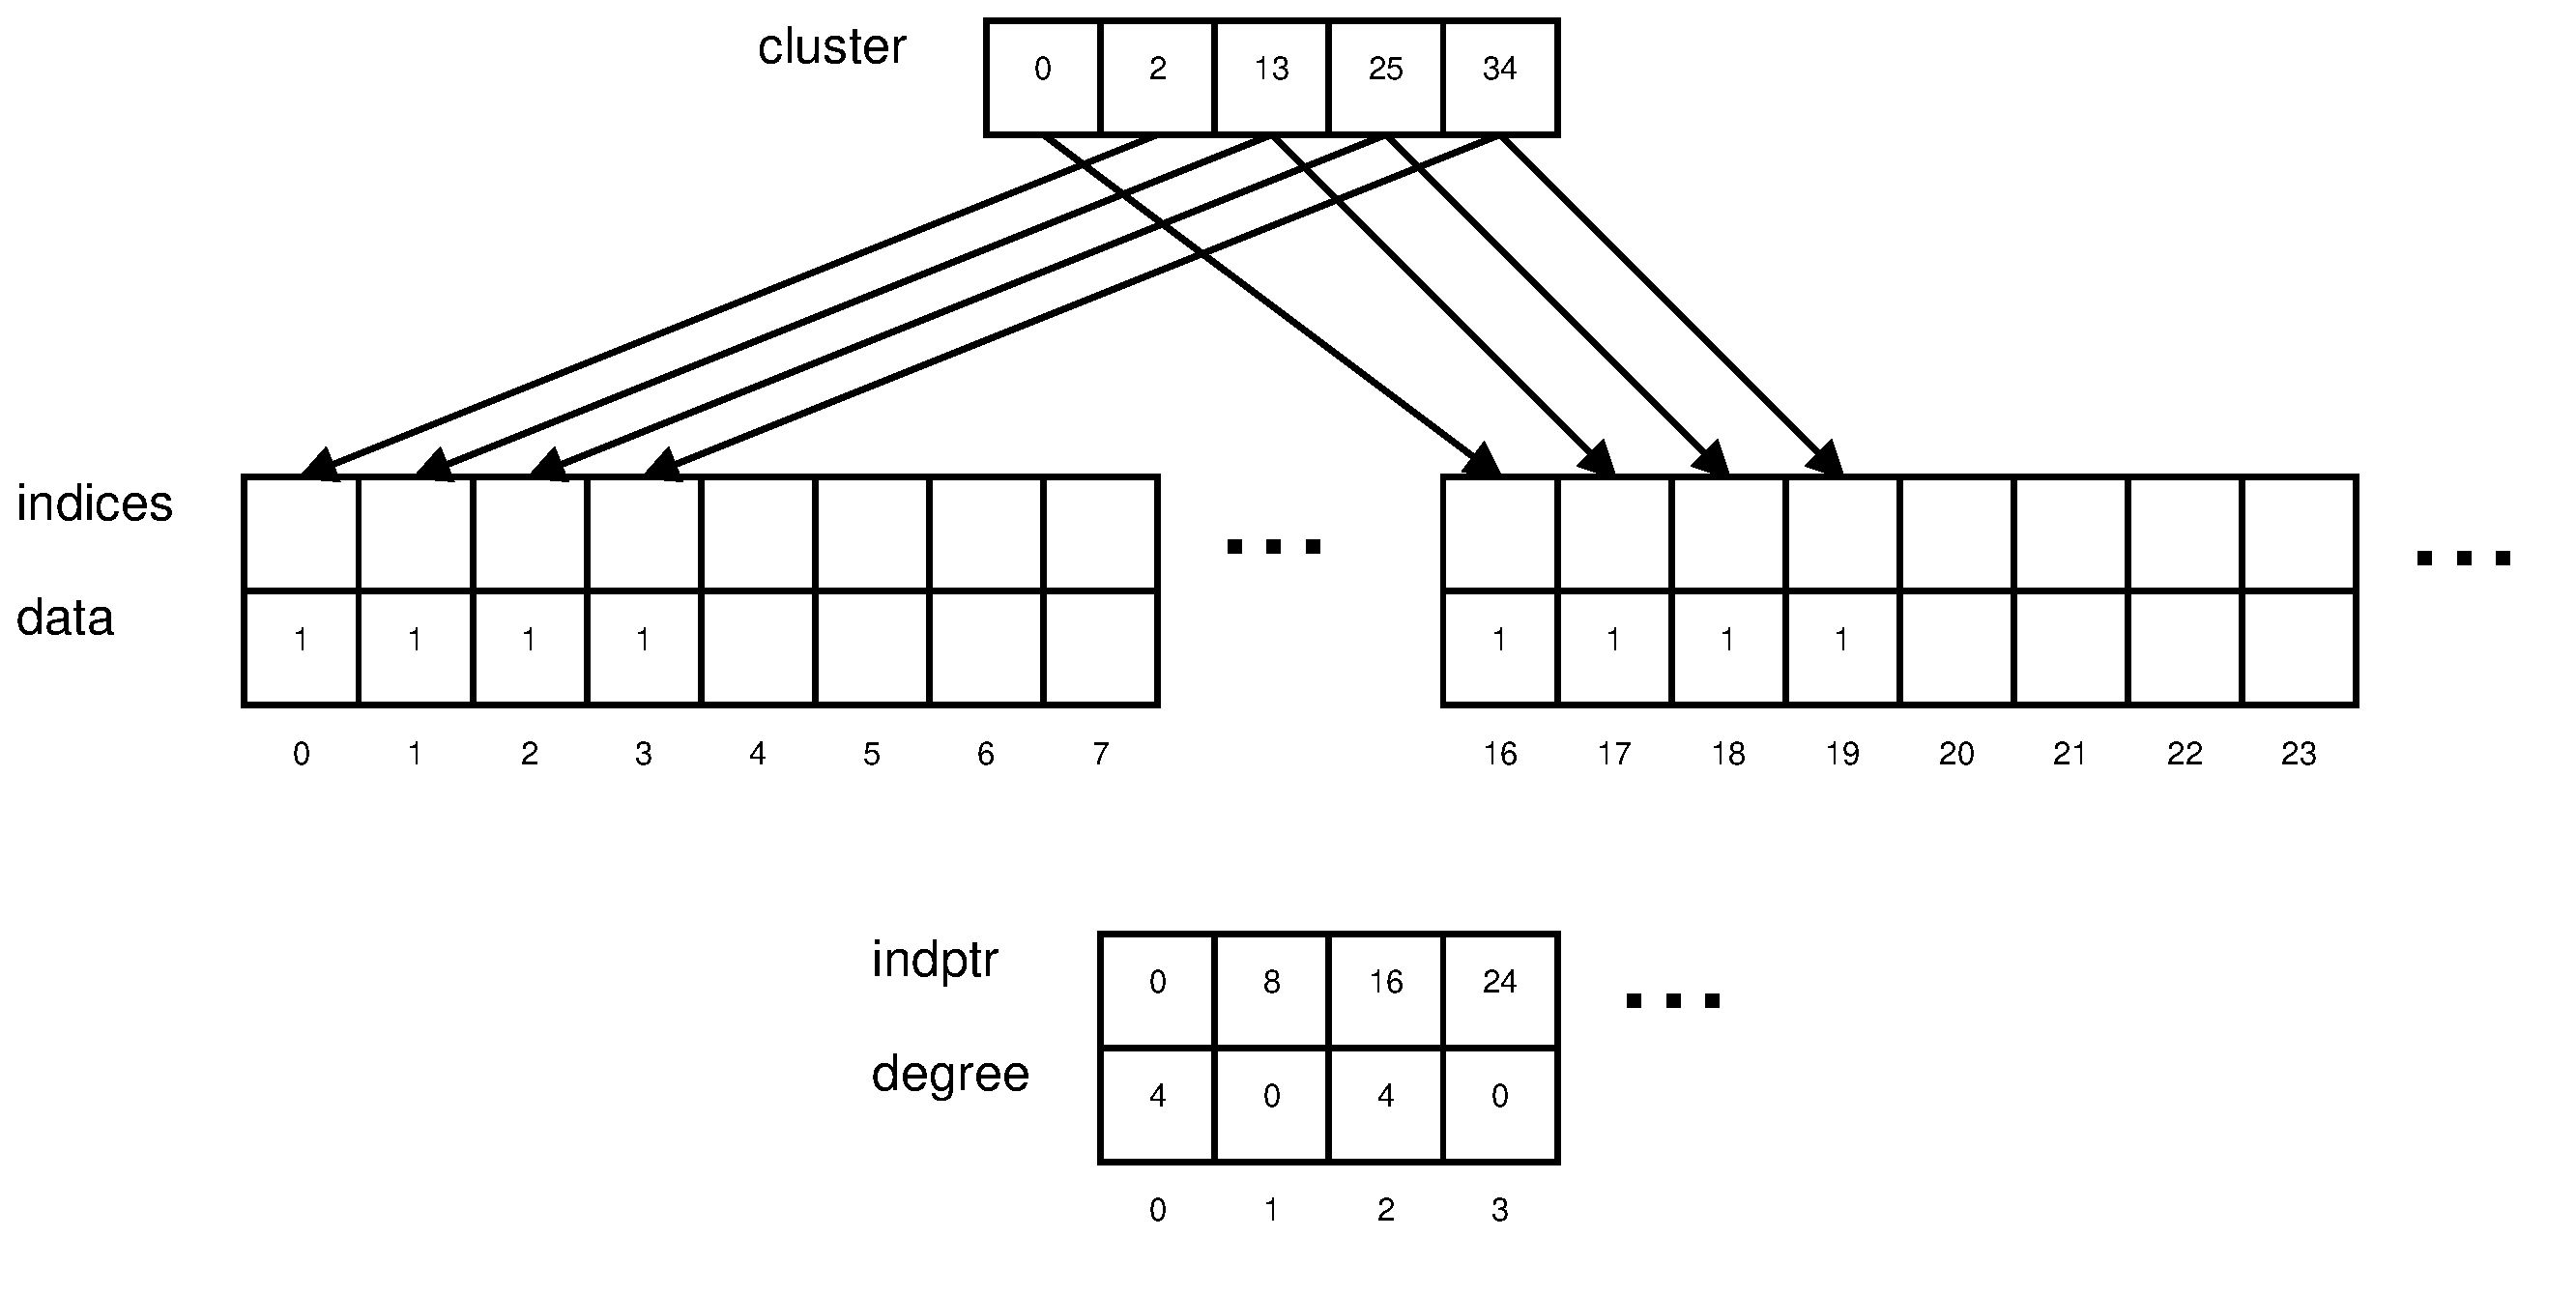
\includegraphics[width=\textwidth]{methodology/eac_csr_first_part}
\caption{Inserting a cluster of the first partition in the co-association matrix.}
\label{fig:first part}
\end{figure}

For the remaining partitions, the process is different.
Now, it is necessary to check if an association already exists.
For each pattern in a cluster it is necessary to add or increment the association to every other pattern in the cluster.
This is described in Algorithm \ref{alg:eac csr update cluster}.


\begin{algorithm}
\caption{Update matrix with cluster.}\label{alg:eac csr update cluster}
\begin{algorithmic}[1]
\Procedure{update\_cluster}{$indices, data, indptr, degree, cluster, max\_assocs$}
\For{$pattern$ $\mathbf{n}$ $in$ $cluster$}
	\For{$every$ $other$ $pattern$ $\mathbf{na}$ $in$ $cluster$}
		\State{$ind$ $=$ $binary\_search(na, indices,$$interval$ $of$ $n$ $in$ $indices)$}
		\If{$ind \ge 0$}
			\State{$increment$ $data[ind]$}
		\Else
            \If{$maximum$ $assocs$ $not$ $reached$}
			    \State{$add$ $new$ $assoc.$ $with$ $weight$ $1$}
            \EndIf
		\EndIf
	\EndFor
\EndFor
\EndProcedure
\end{algorithmic}
\end{algorithm}

Binary search is used to search for the association in the \emph{indices} array in the interval corresponding to a specific row (or pattern).
This is necessary because it is not possible to index directly a specific position of a row in the CSR format.
Since a binary search is performed $(ns - 1)^2$ times for each cluster, where $ns$ is the number of patterns in any given cluster, the indices of each pattern must be in a sorted state at the beginning of each partition insertion.
Two strategies for sorting were devised.
The \underline{first strategy} is to just insert the new associations at the end of the \emph{indices} array (in the correct interval for each pattern) and then, at the end of processing each partition, use a sorting algorithm to sort all the patterns' intervals in the \emph{indices} array.
This was easily implemented with existing code, namely using \emph{NumPy}'s \emph{quicksort} implementation, which has an average time complexity of $O(n \log n)$

The \underline{second strategy} is more complex.
It results from the observation that, if one could know in which position each new association should be inserted, it would be possible to move all old associations to their final sorted positions and insert the new ones.
Furthermore, this would be done in an efficient manner with minimum number of comparisons (and thus branches in the execution of the code).
For this end, the implemented binary search returns the index of the searched value (key) if it is found or the position for a sorted insertion of the key in the array, if it is not found.
In reality, it returns $-ind -1$ if it is not found, where $ind$ is the index for sorted insertion.
This means that the position where each new association should be inserted is now available.
New associations are stored in two auxiliary arrays of size $max\_assocs$: one (\emph{new\_assoc\_ids}) for storing the patterns of the associations and the other (\emph{new\_assoc\_idx}) to store the indices where the new associations should be inserted (the result of the binary search).
The process is illustrated with an example in Fig. \ref{fig:normal part}, detailed in Algorithm \ref{alg:eac csr sort cluster} and explained in the following paragraph.

After each pass on a cluster (adding or incrementing all associations to a pattern in the cluster), the new associations have to be added to the pattern's \emph{indices} interval in a sorted manner.
The number of associations corresponding to the $i$-th pattern (\emph{degree[i]}) is incremented by the amount of new associations to be added.
%The new interval of the \emph{indices} array belonging to the $i$-th pattern now has \emph{degree[i]} plus the number of new associations.
An element is added to the end of the \emph{new\_assoc\_idx} array with the value of \emph{degree[i]} so that the last new association can be included in the general cycle.
During the sorting process a pointer to the current index to add associations $o\_ptr$ is kept ( it is initialized to the new total number of associations of a pattern).
The sorting mechanism looks at two consecutive elements in the \emph{new\_assoc\_idx} array, starting from the end.
If the $i$-th element of the \emph{new\_assoc\_idx} array is greater or equal than the $(i-1)$-th element, then all the associations in the \emph{indices} array between them (including the first element) are shifted to the right by $i$ positions. %are copied to the end of the \emph{indices} interval, i.e. they are shifted to the right by $i$ positions.
Then, or in case the comparison fails, the $(i-1)$-th element of the \emph{new\_assoc\_ids} is copied to the \emph{indices} array in the position specified by \emph{o\_ptr}.
The \emph{o\_ptr} pointer is decremented anytime an association is written in the \emph{indices} array.

\begin{figure}[hbtp]
\centering
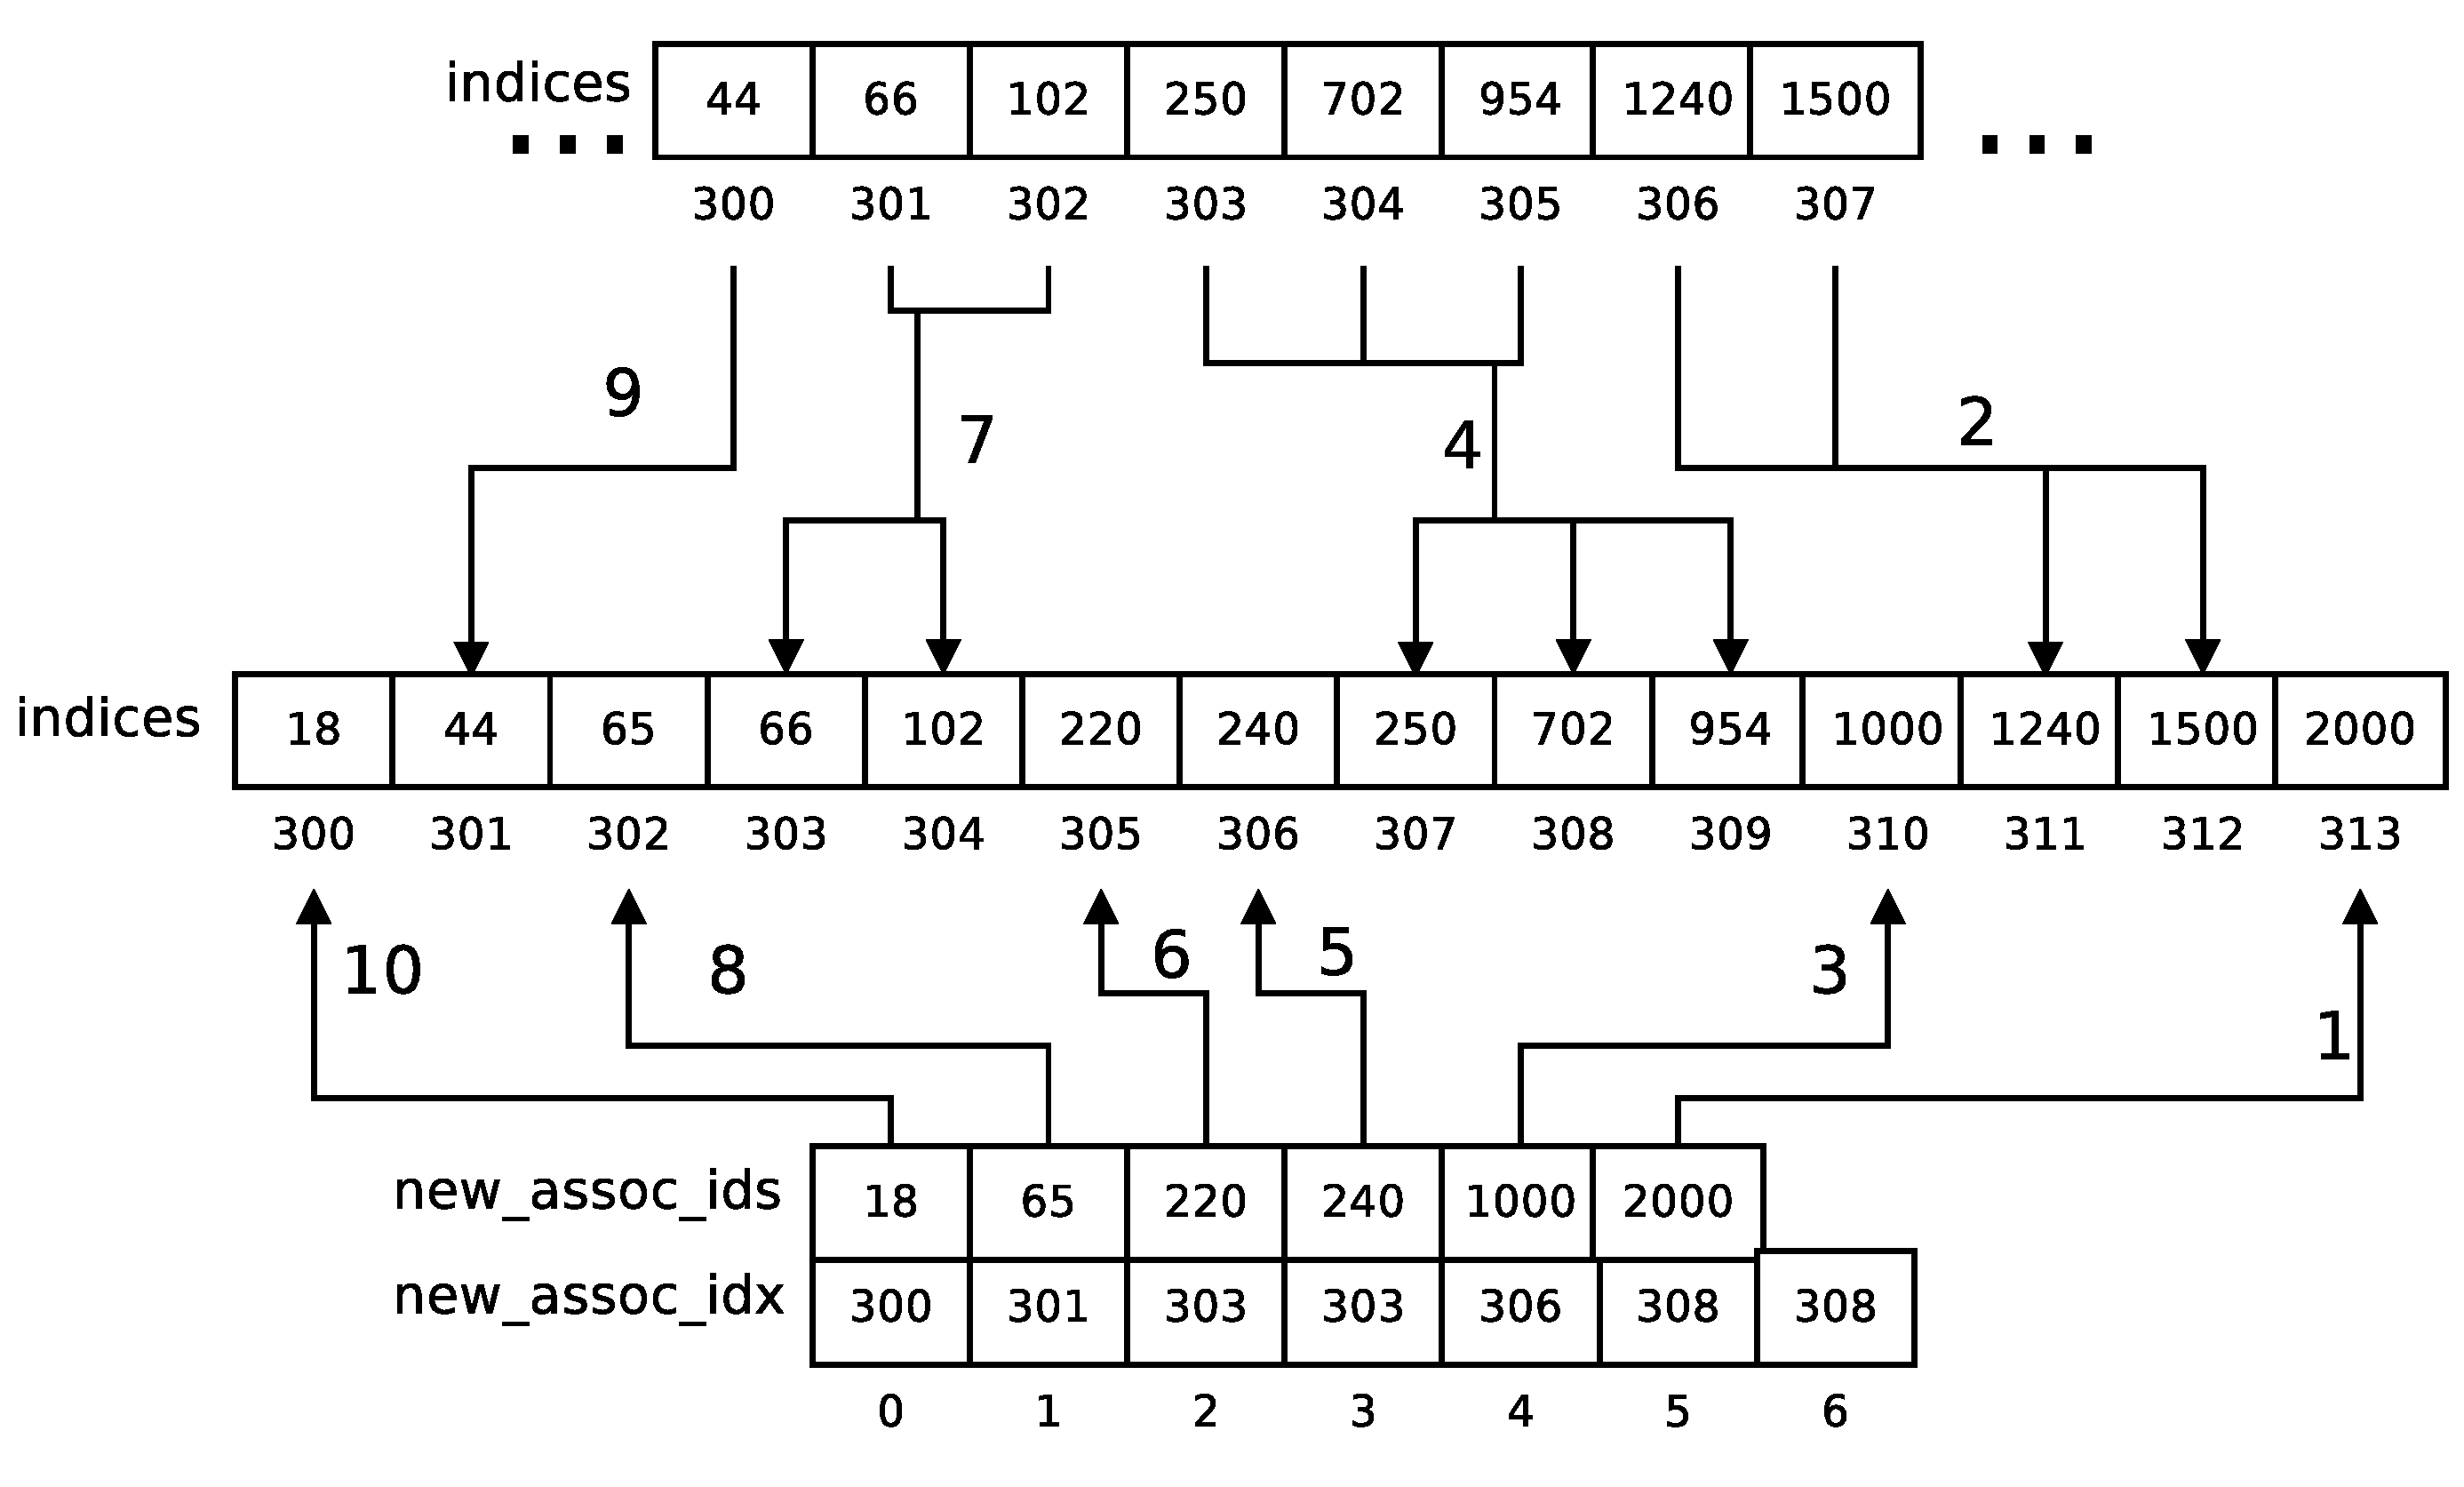
\includegraphics[width=\textwidth]{methodology/sorted_insert}
\caption{Inserting a cluster from a partition in the co-association matrix. The arrows indicate to where the indices are moved. The numbers indicate the order of the operation.}
\label{fig:normal part}
\end{figure}

\begin{algorithm}
\caption{Sort the \emph{indices} array in the interval of a pattern $n$.}\label{alg:eac csr sort cluster}
\begin{algorithmic}[1]
\Procedure{sort\_indices}{$indices, data, indptr, degree, n, new\_assocs\_ptr, new\_assocs\_ids, new\_assocs\_idx$}
\State{$new\_assocs\_idx[new\_assocs\_ptr] = indptr[n] + degree[n]$}
\State{$i = new\_assocs\_ptr$}
\State{$o\_ptr = indptr[n] + new\_assocs\_ptr + degree[n] - 1$}
\While{$i \ge 1$}
	\State{$start\_idx = new\_assocs\_idx[i - 1]$}
	\State{$end\_idx = new\_assocs\_idx[i] - 1$}

    \While{$end\_idx >= start\_idx$}
        \State{$indices[o\_ptr] = indices[end\_idx]$}
        \State{$data[o\_ptr] = data[end\_idx]$}
        \State{$end\_idx -= 1$}
        \State{$o\_ptr -= 1$}
    \EndWhile
    \State{$indices[o\_ptr] = new\_assocs\_ids[i - 1]$}
    \State{$data[o\_ptr] = 1$}    
    \State{$o\_ptr -= 1$}
    \State{$i -= 1$}
\EndWhile

\EndProcedure
\end{algorithmic}
\end{algorithm}

\subsection{EAC CSR Condensed}

The co-association matrix is symmetric, which means that only half is necessary to describe the whole matrix.
That fact has consequences on both memory usage and computational effort on building the matrix.
It translates in a asymptotical reduction to $50\%$ of the original required memory.
Furthermore, only half the operations are made since only half the matrix is accessed, which also accelerates the building of the matrix.
There is, however, a small overhead for translating the two dimensional index to the single dimensional index of the upper triangle matrix.
When using a sparse matrix according to the EAC CSR scheme described above, there is no direct memory usage reduction.
However, the number of binary searches performed by inserting new associations is half which has a significant impact on the computation time relative to the complete matrix.

Even though there is no direct memory reduction for switching to the condensed matrix form, this scheme does open possibilities for it.
Previously, the number of associations for each pattern (number of non zero values in each row) remained constant throughout the whole set of patterns.
However, using a condensed scheme means that the number of associations decreases as one steps further to the end of the set. %, i.e. closer to the bottom the co-association matrix.
An example of this can be seen in the plot of the number of associations per pattern in a complete and condensed matrix of Fig. \ref{fig:coassoc degree}.
It is clear that, since the number of associations that is actually stored in the matrix decreases throughout the matrix, the pre-allocated memory for each pattern can decrease accordingly.
One possible strategy, illustrated in Fig. \ref{fig:coassoc degree}, is to decrease the maximum number of associations linearly.
In the example, the first 5\% of patterns have the 100\% of the maximum number of associations and it decreases linearly until 5\% of the maximum number of associations for the last pattern.

Table \ref{tab:mat type memory} shows the memory usage of the different co-association matrix strategies in the general case and for an example of 100000 patterns.
The memory consumption for the \emph{sparse condensed linear} type of matrix if given for the parameters presented above for Fig. \ref{fig:coassoc degree}.

\begin{table}[hbtp]
\centering
\caption{Memory used for different matrix types for the generic case and a real example of 100000 patterns. The relative reduction (R.R.) refers to the memory reduction relative to the type of matrix above, the absolute reduction (A.R.) refers to the reduction relative to the full complete matrix.}
\label{tab:mat type memory}
\begin{tabular}{lrrrr}
\toprule
\textbf{Type of matrix}          & \textbf{Generic}                & \textbf{Memory {[}MBytes{]}}    & \textbf{R.R.} & \textbf{A.R.} \\
\midrule% \hline
Full complete           & $N^2$                  & $9536.7431$              & -                  & -             \\
Full condensed          & $\frac{N(N-1)}{2}$     & $4768.3238$              & $0.4999$     & $0.4999$      \\
Sparse constant         & $ N \times max\_assocs$ & $678.8253$               & $0.1423$           & $0.0711$      \\
Sparse condensed linear & $ 0.54 \times N \times max\_assocs$ & $372.8497$               & $0.5492$           & $0.0390$      \\
\bottomrule
\end{tabular}
\end{table}


\begin{figure}[hbtp]
\centering
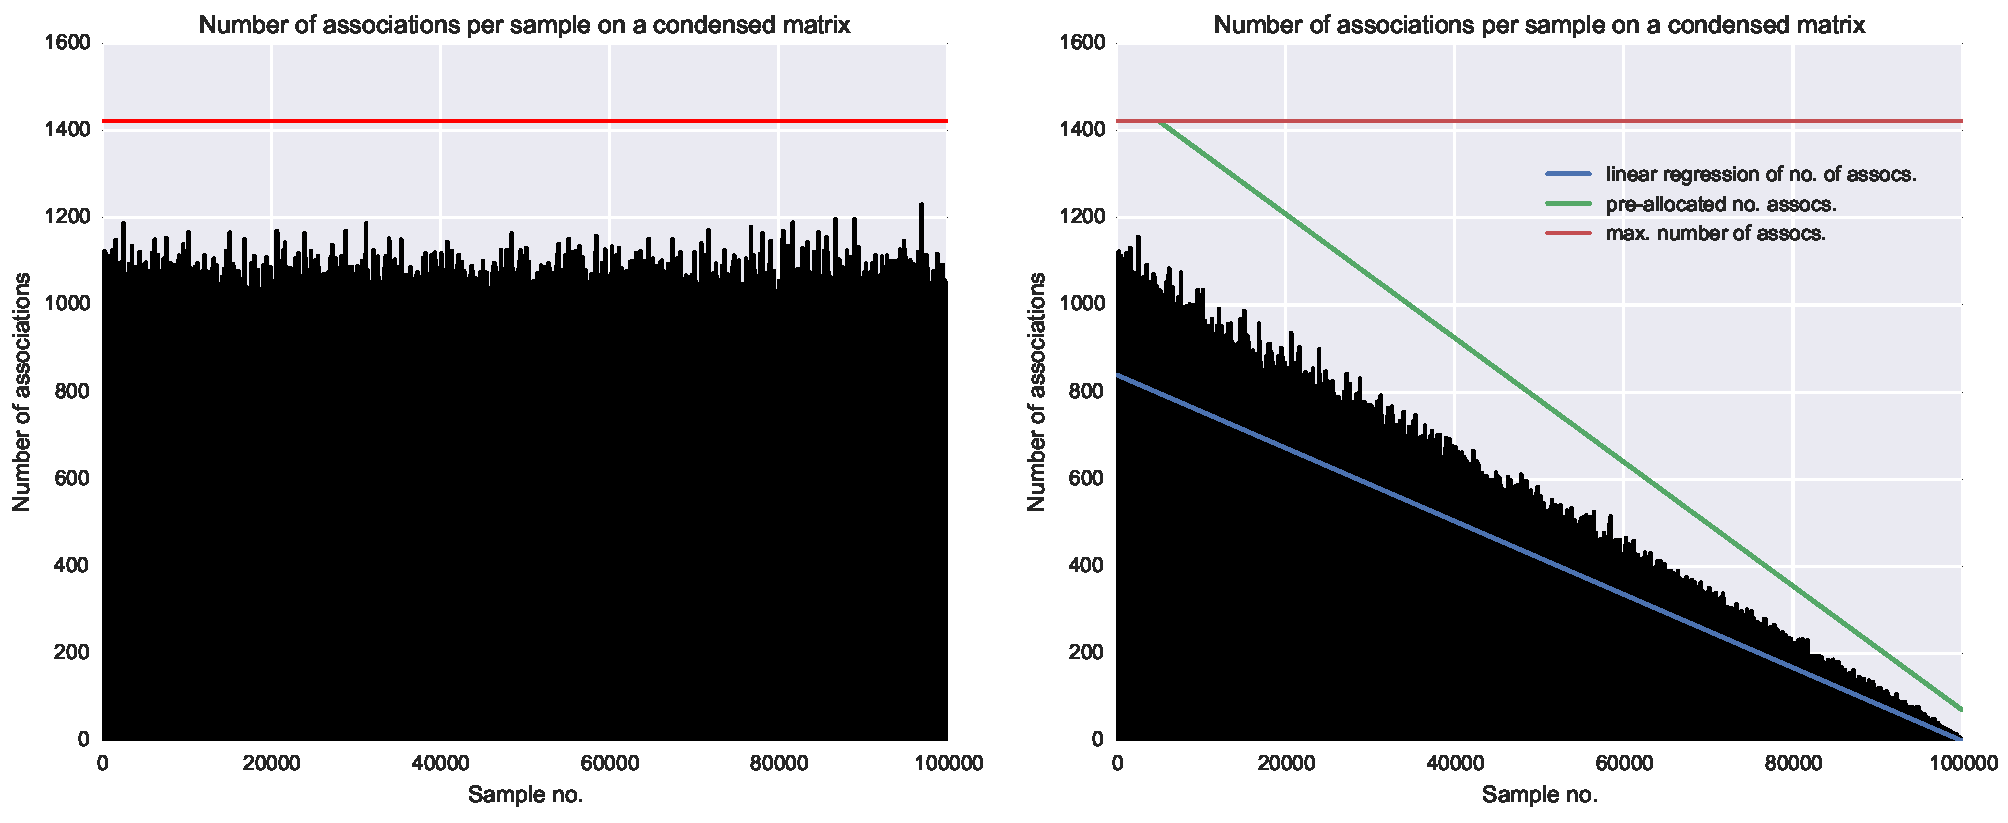
\includegraphics[scale=0.45]{methodology/eac_csr_cond_full_degree_100k}
\caption{The left figure shows the number of associations per pattern in a complete matrix; the right figure shows the number of associations per pattern in a condensed matrix. Dataset used is a bidimensional mixture of 6 Gaussians with a total of $100 \: 000$ patterns.}
\label{fig:coassoc degree}
\end{figure}


\section{Final partition recovery}

This section will present the considered candidates for the final step of EAC.
A GPU version of SL is described in section \ref{sec:sl gpu}.
External algorithms are a candidate solution and this approach is presented in section \ref{sec:sl disk}.
This solution is based on storing the co-association matrix on disk, performing the expensive computation (memory and speed wise) of \emph{argsort} and then processing the matrix in batches until the final MST is extracted.

\subsection{Single-Link and GPGPU}
\label{sec:sl gpu}
% introduction to the procedure of SL with MST
Single-Link is an inherently sequential algorithm which means an efficient GPU version is hard to implement.
However, SL can be performed by computing the MST and cutting edges until we have the desired number of clusters, as described in chapter \ref{chapter:stateofart}.
Considerable speed-ups are reported in the literature for MST solvers in the GPGPU paradigm.
The considered solution uses the efficient parallel variant of Borůvka's algorithm \cite{Sousa2015}.
After the necessary pruning of the MST edges has been performed to achieve the desired number of clusters, the output MST is fed to the labeling algorithm which will provide the final clustering.

\subsubsection{Generating the MST}
% explain modification to the MST algorithm to accept unconnected graphs
The output of the Borůvka's algorithm is a list of the indices of the edges constituting the MST. 
These indices point to the \emph{destination} of the original graph. 
The original algorithm \cite{Sousa2015} assumes connected graphs, but this is not guaranteed in EAC's co-association matrix.
In graph theory, given a connected graph $G = (V,E)$, there is a path between any $s,t \in V$, where $V$ is the set of vertices in $G$ and $E$ is the set of edges that connects the vertices.
In an unconnected graph, this is not the case and unconnected subsets are called components, i.e. a connected component $C \subset V$ ensures that for each $u,v \in C$ there is a path between $u$ and $v$.
The present implementation follows the original literature \cite{Sousa2015} for the exception of a modification that allows it to process unconnected graphs.
The issue of unconnected graphs was solved in the first step (finding the minimum edge connected to each vertex or supervertex). 
If a vertex has no edges connected to it (an outdegree of 0 since all edges are duplicated to cover both directions) then it is marked as a mirrored edge. 
This means that the independent components will be marked as supervertices in all subsequent iterations of the algorithm. 
The overhead of having these redundant vertices is low since the number of independent components is typically low compared to the number of vertices in the graph and the processing of such vertices is very fast.
As a consequence, the stopping criteria becomes the lack of edges connected to the remaining vertices, which is the same as saying that all elements of the \emph{outdegree} array are zero. 
This condition can be checked as a secondary result of the computation of the new \emph{first\_edge} array. 
This step is performed by applying an exclusive prefix sum over the \emph{outdegree}. 
The prefix sum was implemented in such a way that it returns the sum of all elements, which translates in very low overhead to check this condition.
The final output is the MST array and the number of edges in the array. 
The later is necessary because the number of edges will be less than $|V|-1$ when independent components exist, and also because the MST array is pre-allocated in the beginning of the algorithm when the number of edges is not yet known.

\subsubsection{Number of clusters and pruning the MST}
% cutting edges
The number of clusters can be automatically computed with the lifetime technique or be supplied. 
Either way, a list (\emph{mst\_weights}) with the weights of each edge of the MST is compiled and ordered.
The list of edges is also ordered according to the order of the \emph{mst\_weights}. 
If the number of clusters $k$ was given, the algorithm removes the $k - 1$ heaviest edges. 
If there are independent components inside the MST those are taken into consideration before removing any edges.
If the number of clusters $k$ is higher than the number of independent components the final number of clusters will be the number of independent components.

To compute the number of clusters (which results in a truly unsupervised method) the lifetimes are computed.
In the traditional EAC, lifetimes are computed on the weights of the clusters by the order they are formed.
With the MST, the lifetimes are computed over the ordered \emph{mst\_weights} array, which is equivalent.
If there are independent components, an extra lifetime is computed from the representative weight connecting independent components.
This lifetime will serve as the threshold between choosing the number of independent components as the number of clusters or looking into the lifetimes within the MST.
This is because links between independent vertices are not included in the MST.
For this reason, the lifetime for going from independent edges to the heaviest link in the MST (where the first cut would be performed) is computed separately.
If the maximum lifetime within the MST is bigger than the threshold, than the number of clusters is computed as in traditional EAC plus the number of independent components.
Otherwise, the independent components will be the final clusters.
Most of this process can be done by the GPU. 
Library kernels were used to sort the array and compute the $arg max$, and a simple kernel was used to compute the lifetimes.

\subsubsection{Building the new graph}
The final MST (after performing the pruning) is then converted into a new, reduced graph.
The function responsible for this produces a graph in CSR format from the original graph and the final selection of edges composing the MST.
The function has to count the number of edges for each vertex, compute the origin vertex of each edge (the original \emph{destination} array only contains the destination vertices) and, with that information, build the final graph.
This process can be done by the GPU with simple mapping kernels and a modified binary search for determining the origin vertex.

\subsubsection{Final clustering}
The last step is computing the final clusters.
Any incision in the MST translates in independent components in the constructed graph.
This means that the problem of computing the clusters translates into a problem of finding independent connected components in a graph, a problem that usually goes by the name of Connected Component Labeling.
To implement this part in the GPU, the aforementioned Borůvka algorithm was modified to output an array \emph{labels} of length $|V|$ such that the $i-th$ position contains the label of the $i-th$ vertex.
To this effect, the flow of the algorithm was slightly altered as shown in Figure \ref{fig:connected comps flow}. 
The kernel dealing with the MST was removed and a kernel to update the labels at each iteration, shown in Algorithm \ref{alg:comp_labels}, was implemented.
In the first iteration of the algorithm the converged colors are copied to the labels array.
In every iteration the kernel to update the labels takes in the propagated colors and the array with the new vertex IDs.
For each vertex in the array, the kernel first takes in the color of the current vertex and maps it to the new color (one should notice that the color is actually a vertex ID and that that vertex has had its color updated).
Afterwards, the kernel maps the new color with the new vertex ID that color will take, to keep consistency with future iterations.

\begin{figure}[hbtp]
\centering
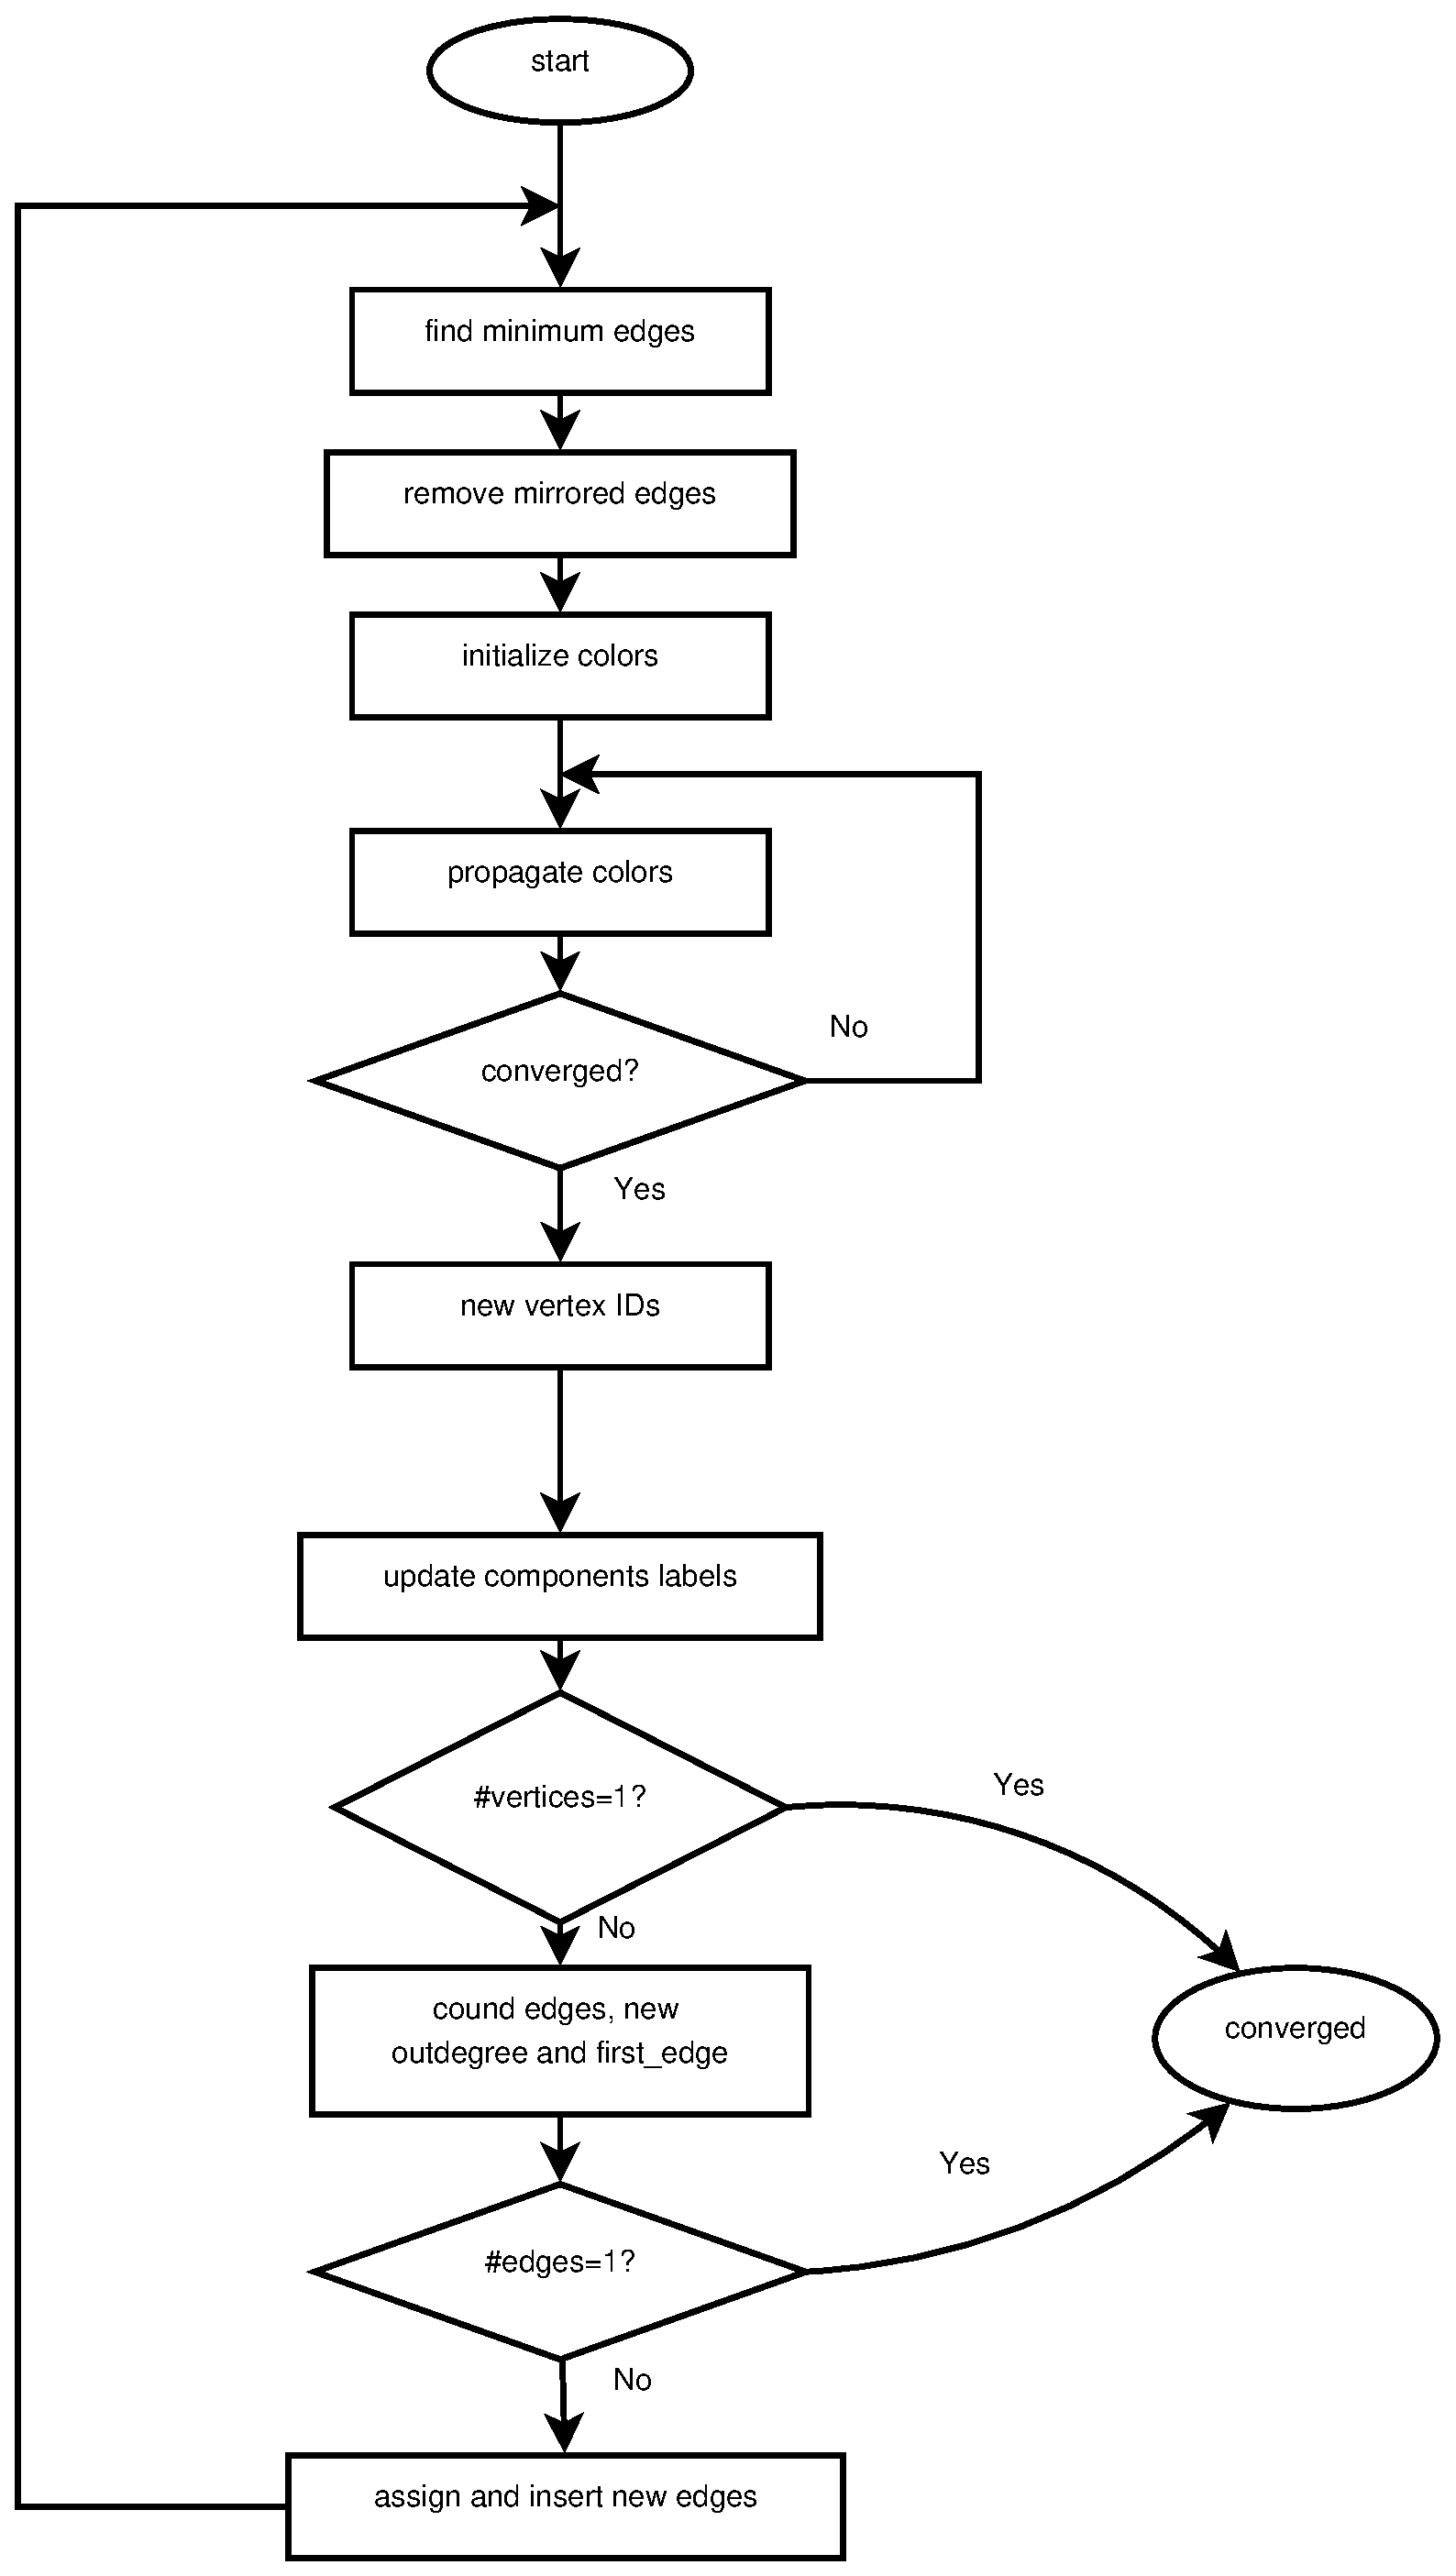
\includegraphics[scale=0.5]{methodology/connected_components_boruvka_flow.eps}
\caption{Diagram of the connected components labeling algorithm used.}
\label{fig:connected comps flow}
\end{figure}


%
% describe connected components algorithm
% how it copies colors in the first time
% and then just updates the labels with the new vertex IDs
%
% put flowchart and pseudocode


\begin{algorithm}
\caption{Update component labels kernel}\label{alg:comp_labels}
\begin{algorithmic}[1]
\Procedure{update\_labels}{$vertex\_id, labels, colors, new\_vertex$}
\State $curr\_color \gets labels[vertex\_id]$
\State $new\_color \gets colors[curr\_color]$
\State $new\_color\_id \gets new\_vertex[new\_color]$
\State $labels[vertex\_id] \gets new\_color\_id$
\EndProcedure
\end{algorithmic}
\end{algorithm}



\subsubsection{Memory transfer with the GPU}
The whole algorithm of computing the SL clustering has been implemented in the GPU, having the optimization of memory utilization in mind.
The control logic is the only thing that is processed by the host. 
Transferring the initial graph is the most relevant memory transfer.
It has to be transfered twice: first for computing the MST and then to build the processed MST graph.
This happens because the initial device arrays used for the graph are deallocated to give space for the arrays of subsequent iterations of the MST algorithm.
This implementation design had in mind memory consumption and could easily be avoided with the cost of having to store the bigger initial graph for the entire duration of the MST computation, which might be worthwhile if the GPU memory is abundant.
The final labels array is transfered back to the host in the end of computation, but its size is small relative to the size of the original graph.
Furthermore, because the control logic is processed by the host and it is dependent on some values computed by the device, extra memory transfers of single values (e.g. number of vertices and number of edges on each iteration) are necessary.
These, however, may be safely dismissed since they are of little consequence in the overall computation time.


\subsubsection{Contrast between implementations}

At this point it should be noted, for future reference, the contrast between the technology stack used by \citet{Sousa2015} and the one used here.
\citet{Sousa2015} used the native CUDA language to program the GPUs and highly optimized libraries.
The implementation in the present work used none of the above.
Accordingly, some performance may be lost.
This if specially true for some highly optimized operations that can be found in some libraries, since those use optimization mechanisms that are not available in the used CUDA API offered by the Numba package.
An evaluation of the interoperability between the technology stacks was made but, currently, this does not seem feasible.
Nevertheless, and whenever possible, we tried to close the gap so that these shortcomings become less noticeable in the overall performance.

\subsection{Single-Link and external memory algorithms}
\label{sec:sl disk}


The co-association matrix can become very large for large datasets.
Even using the EAC CSR method to reduce memory usage, it occupies a significant portion of main memory.
Furthermore, the algorithm to compute a MST brings additional space complexity that make it infeasible to perform the final partition recovery on a large co-association matrix in main memory.
External memory algorithms address this issue.
% out of core processing %TODO check
External memory algorithms (or out-of-core algorithms) refers to algorithms that are based on disk (or other large capacity but typically low latency storage technology), usually by loading small batches to main memory, processing them, saving the results and repeating until the whole computation is done.
This section describes the process of building the MST with low memory usage.
The details of converting the MST in a Single-Link clustering are described in chapter \ref{chapter:stateofart} and omitted here.

\subsubsection{Kruskal's algorithm and implementation}

% Kruskal algorithm
The sequential MST algorithm used was Kruskal \cite{kruskal1956shortest}, which describes three approaches for finding a MST.
The SciPy library offers an efficient implementation for the following construct (taken directly from the original paper of Kruskal's algorithm):
\begin{displayquote}
CONSTRUCTION A. Perform the following step as many times as possible: Among the edges of G not yet chosen, choose the shortest edge which does not form any loops with those edges already chosen. Clearly the set of edges eventually chosen must form a spanning tree of G, and in fact it forms a shortest spanning tree.
\end{displayquote}
If the graph is connected, the algorithm will stop before processing all edges when $|V| - 1$ edges are added to the MST.
Within the EAC context, it is very common for the co-association graph to have independent components which translates in every edge being processed.
It should be noted that this implementation works on a sparse matrix in the CSR format.

One of the main steps of the implementation is computing the order of the edges of the graph without sorting the edges themselves, an operation called \emph{argsort}.
To illustrate this, the \emph{argsort} operation on the array $ \left [  4 , 5 , 2 , 1, 3 \right ]$ would yield $ \left [  3 , 2 , 4, 0 , 1 \right ]$ since the smallest element is at position 3 (starting from 0), the second smallest at position 2, etc.
This operation is useful to avoid computing the shortest edge in every iteration.
Doing so would increase time complexity since a sorting algorithm may have an average time complexity to $O(n log n)$ (QuickSort algorithm) while a single minimum has a time complexity of $O(n)$.
Computing the minimum at every iteration when every edge must be processed means that there will be $|E|$ iterations and so the total time complexity for the minimum operation alone will be $O(E ^ E)$ if processed edges are not removed or $O(E!)$ if they are.
These are much higher than Kruskal's time complexity of $O(E log E)$.
The result of this operation is an array of length $|E|$ (i.e. the number of associations in EAC), which means it will occupy at least the same size as the array containing the weights of the edges.
However, the total size is typically 8 times larger for EAC since the data type of the weights uses only one byte and the number of associations is very large, forcing the use a 8 byte integer for the \emph{argsort} output array.
This is the real motivation to store the co-association matrix in disk and use an external sorting algorithm.

\subsubsection{Kruskal's implementation with an external sorting algorithm}

The \emph{PyTables} library \cite{pytables}, which is built on top of the \emph{HDF5} format \cite{hdf5}, was used for storing the graph, performing the external sorting for the \emph{argsort} operation and loading the graph in batches for processing.
This implementation starts by storing the CSR graph to disk.
However, instead of saving the \emph{indptr} array directly, an expanded version is stored instead.
The expanded version will be of the same length as the \emph{indices} array and the $i$-th element contains the origin vertex (or row) of the $i$-th edge.
This way, a binary search for discovering the origin vertex becomes unnecessary.

Afterwards, the \emph{argsort} operation is performed by building a completely sorted index (CSI) of the \emph{data} array of the CSR matrix.
The details of CSI implementation fall outside the scope of this dissertation but are explained in further detail in \cite{AltetiAbad2007}.
It should be noted that the arrays themselves are not sorted.
Instead, the CSI allows for a fast indexing of the arrays in a sorted manner (according to the order of the edges).
%The CSI will be used to retrieve edges from the stored graph in a sorted manner.
The process of building the CSI has a very low main memory usage that can be disregarded.

The SciPy implementation of Kruskal's algorithm was modified to work with batches of the graph.
This was easily implemented just by making the additional data structures used in the building of MST persistent between calls of the function.
The new implementation loads the graph in batches and in a sorted manner, e.g. first load a batch of the 1000 smallest edges, then a batch of the next 1000 smalled edges, etc.
Each batch must be processed sequentially since the edges must be processed in a sorted manner, which means that there is no possibility for parallelism in this process.
Typically, the batch size is a very small fraction of the size of the edges, which means that the total memory usage for building the MST is overshadowed by the size of the co-association matrix.
The time complexity for building the CSI is higher than computing the \emph{argsort} operation, but the formal time complexity is not reported in the source \cite{AltetiAbad2007}.
As an example, for a $500 \: 000$ pattern set the SL-MST approach took $54.9$ seconds while the external memory approach took $2613.5$ seconds - two orders of magnitude higher.

\section{Overview of the developed work}
\label{sec:methodology overview}

This chapter exposed a great deal of the actual developed work.
It covered solutions and implementations related to the three phases of EAC.
For the production of the ensemble, two quantum clustering algorithms and a GPU parallel K-Means variant were implemented.
These are algorithms existing in the literature (presented in chapter \ref{chapter:stateofart}) and implementation details were presented when relevant.
For addressing the computation complexity of the second phase of EAC, a novel method \textbf{EAC CSR} for building the co-association matrix was designed and implemented.
Finally, three approaches are presented for the last phase of EAC.
An implementation of a parallel GPU MST algorithm based on Borůvka's algorithm was presented along with a labeling algorithm for a forest of MSTs.
Also, an implementation of SL-MST based on Kruskal's algorithm and an external memory variant of it were presented.
The core of the external memory variant is based on using an external algorithm for sorting a very big array stored in disk and, although this is not something new, its application within the SL clustering framework was not found in literature.

% \subsubsection{Effects on the EAC algorithm}

% This section described two implementations for building a MST from a CSR graph.
% As mentioned before, using an MST based approach to Single-Link (SL-MST) already reduces significantly its computational complexity by only processing non-zero edges, which compose only a fraction of a co-association matrix in EAC.
% The implementation of SL-MST is based on the SciPy library and is explained above. 
% Still, the space complexity of MST-based SL can be too high for large datasets.
% This motivated the use of external algorithms using the PyTables library.
% The core concept of this approach is to store the co-association graph in disk and building a sorted index for later use.
% The sorted index is used for 



\section{Guidelines for using the different solutions}
\label{sec:solution}

The final proposed solution is composed by the parallel K-Means implementation described, the EAC CSR method and the external memory variant for performing Single-Link.
The implementations have several parameters available for tinkering.
A general guideline of what is available and when should it be used is presented in this chapter.

It is recommended that the execution of the parallel K-Means algorithm be done with the optimized memory transfer, so as to minimize communication between GPU and host.
When the combined size of the dataset, centroid set, labels and distance arrays exceed the available device memory, the pure sequential version of K-Means should be used.
An optimized sequential version is offered alongside the implementation of its parallel counterpart.

The choice of parameters of the method for building the co-association matrix is a simple one to make.
The available choices are:

\begin{itemize}
	\item if the matrix should be condensed (filling only the upper triangular) or not, 
	\item if the matrix should be sparse or not;
	\item within the sparse matrices, if a constant or linear memory allocation should be used.
\end{itemize}

The condensed version of the matrix is always preferred.
Not only does it occupy less than half of the memory, it takes less time to build and completely describes the co-association matrix.
Furthermore, when this is paired with a sparse strategy, the final clustering is also nearly twice as fast.
A sparse representation should be chosen whenever $n (n-1) / 2$ times the size of the data type used (typically unsigned 1 byte integer) exceeds the available memory, where $n$ is the number of patterns in the dataset.
The linear memory allocation is the ideal choice when a sparse representation of the condensed matrix is used, since half the memory is saved.

For the final clustering, the SLINK algorithm must be paired with a fully allocated matrix while the SL-MST strategy must be paired with a sparse representation.
Then, the final choice to make is if one should use the main memory approach for the final Single-Link clustering or the external memory approach.
Here, again, the decision is straightforward.
Typically if the sparse co-association matrix exceeds half of the available main memory, a external memory approach should be chosen.
The reason for this is that one of the crucial steps of the final clustering will almost double the memory used. % add new .tex files for new chapters
%!TEX root = thesis.tex
% \rscpath = contains the path to the resources folder

% \begin{table}[h]
% \centering
% \caption{}

% \label{tab:}
% \end{table}

\chapter{Results and Discussion}
\label{chapter:results}

The present chapter is dedicated to the results relevant to the work produced and their associated interpretation and subsequent discussion.
% Different results are presented, not always directly related to the EAC method.
% Still, the set-up of the tests and experiments was always done with EAC in mind and how one could improve it with different perspectives.
Results include the reviewed quantum clustering algorithms, the parallel GPU K-Means, a brief analysis of sparse matrix building performance, performance analysis of GPU Borůvka, validation of the proposed solution against the original implementation, a thorough study on different properties of EAC and performance of the proposed solution in several large real world data sets.


% % % % % % % % % % % % % % % % % % % % % % % % % % % % % % % % % % % % % % % %
%
%  					RESULTS
%
% % % % % % % % % % % % % % % % % % % % % % % % % % % % % % % % % % % % % % % %

\section{Experimental environment}
\label{sec:system configs}

All experiments were carried out in one of three distinct machines that will be referred to as \textbf{Alpha}, \textbf{Bravo} and \textbf{Charlie}.
Their CPU and GPU hardware configurations are described in Tables \ref{tab:alpha}, \ref{tab:bravo} and \ref{tab:charlie}, respectively.
Besides, Charlie has a \emph{Seagate ST2000DM001} 7200 RPM spinning disk and a \emph{Samsung 840 EVO} Solid State Drive, informations relevant for the third phase of EAC.% with sequential read/write speeds of up to 540/410 MB/s.

Software wise, all machines are running Linux based operating systems.
Alpha and Bravo are using the Ubuntu 14.04 and 12.04, respectively, with a graphical interface.
Whether the machine is running a graphical interface or not is important because the amount of time a GPU kernel can take when the GPU is being used as a display device is severely constrained. %, in the case that it only has one GPU (as is the case with all the machines here presented) the available memory for computation is less than total and there is a limit to how long a CUDA kernel can be executed.
Charlie is running Fedora 21 without a graphical interface.

% SAMSUNG HM641JI
% http://www.farnell.com/datasheets/841934.pdf
% 5400 RPM
% 209.3IOPS


% Mighty4 SSD : http://hexus.net/tech/reviews/storage/58229-samsung-ssd-840-evo-120gb/
% needs booktabs package
% table inside minipage to have footnotes at the end
% system configuration of Samsung RV520.
\begin{minipage}[h]{\hsize}
	\centering
	\captionof{table}{\textbf{Alpha} machine specifications.}
	\begin{tabular}{ccc}
		\toprule[2pt]
												 & \textbf{CPU}      & \textbf{GPU} \\ \midrule
		\textbf{\# Devices}                      & 1                 & 1            \\ 
		\textbf{Manufacturer}                    & Intel             & NVIDIA       \\ 
		\textbf{Model}                           & i3-2310M          & GT 520M      \\ 
		\textbf{Launch date}                     & Q1'11             & Q1'2011      \\ 
		\textbf{Architecture}                    & Sandy Bridge      & Fermi        \\ 
		\textbf{\# Cores}                        & 2                 & 48           \\ 
		\textbf{Clock frequency {[}Mhz{]}}       & 2100              & 1480         \\ 
		\textbf{L1 Cache}                        & 64KB IC \footnote{Instruction Cache (IC)} + 64KB DC \footnote{Data Cache (IC)} & 16/48 KB/SM \footnote{Each Streaming Multiprocessor has 64 KB of on-chip memory that can be configured as either 16KB of L1 cache and 48 KB of shared memory, or vice versa.}  \\ 
		\textbf{L2 Cache}                        & 512KB             & n/a          \\ 
		\textbf{L3 Cache}                        & 3 MB              & n/a          \\ 
		\textbf{Memory {[}GB{]}}                 & 4                 & 1            \\ 
		\textbf{Max. memory bandwidth {[}Gbps{]}} & 21.3              & 12.8        \\ 
		\bottomrule[2pt]
	\end{tabular}
	\label{tab:alpha}
\end{minipage}
% needs booktabs package
% table inside minipage to have footnotes at the end
% Mighty4 configuration an Instituto de Telecomunicações at 04OCT2015
\begin{minipage}[h]{\hsize}
	\centering
	\captionof{table}{\textbf{Bravo} machine specifications.}
	\begin{tabular}{ccc}
		\toprule[2pt]
												 & \textbf{CPU}      & \textbf{GPU} \\ \midrule
		\textbf{\# Devices}                      & 1                 & 1            \\ 
		\textbf{Manufacturer}                    & Intel             & NVIDIA       \\ 
		\textbf{Model}                           & i7-4930K          & Quadro K600      \\ 
		\textbf{Launch date}                     & Q3'13             & Q1'2013      \\ 
		\textbf{Architecture}                    & Ivy Bridge      &         \\ 
		\textbf{\# Cores}                        & 6                 & 192           \\ 
		\textbf{Clock frequency {[}Mhz{]}}       & 3400              & 876         \\ 
		\textbf{L1 Cache}                        & 192 KB IC \footnote{Instruction Cache (IC)} + 192 KB DC \footnote{Data Cache (IC)} & 16/48 KB/SM \footnote{Each Streaming Multiprocessor has 64 KB of on-chip memory that can be configured as either 16KB of L1 cache and 48 KB of shared memory, or vice versa.} + 48KB DC \footnote{The Kepler architecture has an extra read-only 48KB of Data Cache at the same level of the L1 cache.} \\ 
		\textbf{L2 Cache}                        & 1,5 MB             & 1.5 MB         \\ 
		\textbf{L3 Cache}                        & 12 MB              & n/a          \\ 
		\textbf{Memory {[}GB{]}}                 & 32                & 1            \\ 
		\textbf{Max. memory bandwidth {[}Gbps{]}} & 59,6              & 28,5        \\ 
		\bottomrule[2pt]
	\end{tabular}
	\label{tab:bravo}
\end{minipage}
% needs booktabs package
% table inside minipage to have footnotes at the end
% Mariana configuration an INESC-ID at 04OCT2015
\begin{minipage}[h]{\hsize}
	\centering
	\captionof{table}{\textbf{Charlie} machine specifications.}
	\begin{tabular}{ccc}
		\toprule[2pt]
												 & \textbf{CPU}      & \textbf{GPU} \\ \midrule
		\textbf{\# Devices}                      & 1                 & 1            \\ 
		\textbf{Manufacturer}                    & Intel             & NVIDIA       \\ 
		\textbf{Model}                           & i7 4770K          & K40c      \\ 
		\textbf{Launch date}                     & Q2'13             & Q4'13      \\ 
		\textbf{Architecture}                    & Haswell      & Kepler        \\ 
		\textbf{\# Cores}                        & 4                 & 2880           \\ 
		\textbf{Clock frequency {[}Mhz{]}}       & 3500              & 745         \\ 
		\textbf{L1 Cache}                        & 128 KB IC \footnote{Instruction Cache (IC)} + 128 KB DC \footnote{Data Cache (IC)} & 16/48 KB/SM \footnote{Each Streaming Multiprocessor has 64 KB of on-chip memory that can be configured as either 16KB of L1 cache and 48 KB of shared memory, or vice versa.} + 48KB DC \footnote{The Kepler architecture has an extra read-only 48KB of Data Cache at the same level of the L1 cache.} \\ 
		\textbf{L2 Cache}                        & 1 MB             & 1.5 MB         \\ 
		\textbf{L3 Cache}                        & 8 MB              & n/a          \\ 
		\textbf{Memory {[}GB{]}}                 & 32                & 12            \\ 
		\textbf{Max. memory bandwidth {[}Gbps{]}} & 25,6              & 288        \\ 
		\bottomrule[2pt]
	\end{tabular}
	\label{tab:charlie}
\end{minipage} % Experimental environment
%!TEX root = Thesis.tex

\section{Quantum Clustering}

This section presents performance and validity results of Quantum K-Means and Horn and Gottlieb's algorithm.
All results were obtained using machine Alpha.

\subsection{Quantum K-Means}

The testing was aimed at benchmarking both accuracy and speed.
The input used was synthetic data, namely, Gaussian mixtures with variable number of clusters and features.

The tests were performed using 10 oracles, a qubit string length of 8 and 100 generations per round.
The classical K-Means was executed using the \emph{k-means++} centroid initialization method to make for a fairer comparison, since QK-Means performs several operations (initialization and collapse of oracles) at the beginning of the algorithm.
Furthermore, the performance results for K-Means alone refer to $num.oracles \times num.generations \times factor$ runs, where $factor$ is an adjustable multiplier.
Each test had 20 rounds to allow for statistical analysis of the results. %, since QK-Means executes a classical K-Means for each oracle each generation,
The stopping criteria for all classical K-Means runs was the error between the centroids of two subsequent iterations, more specifically, when the centroids of two iterations differed by less than $0.001$.

All tests were done with 6 clusters (natural number of clusters).
Two tests were done with the two dimensional dataset: one with a $factor=1.10$ (increase initializations by $10\%$) and another with $factor=1$.
These tests will be called T1 and T2, respectively.
The test was done with the six dimensional dataset (T3) using $factor=1.10$.

% table in csv format available in resource directory -->
Performance results are presented in Table \ref{tab:qkmeans times}.
The mean computation time of classical K-Means is an order of magnitude lower than that of QK-Means.
However, the solution chosen in classical K-Means was the one with lowest sum of squared euclidean distances of points to their attributed centroid.
To analyze the influence of the Davies-Bouldin (DB) index, it was computed on all classical K-Means solutions and used as the criteria to choose the best solution.
When this is done, we can see in Table \ref{tab:qkmeans times} that the total time of classical K-Means is actually higher that that of QK-Means in T1 and T3, but this is only due to the 1.10 multiplier on the number of initializations.
In T2, the computation times become very similar with only a 2\% difference between these two variants.
Results show that most computational cost (88\% on T2) lies on the evaluation of the solutions obtained from each oracle, i.e. computing the DB index.
This is a costly but necessary step in this algorithm.

\begin{table}[h]
\centering
\caption{Timing results for the different algorithms in the different tests. Fitness time refers to the time that took to compute the DB index of each solution of classical K-Means. All time values are the average over 20 rounds and are displayed in seconds.}
\begin{tabular}{llrrrr}
\toprule
\textbf{Dataset}               & \textbf{Algorithm} & \textbf{Mean} & \textbf{Variance} & \textbf{Best} & \textbf{Worst} \\
\midrule
\textbf{T1}                    & QK-Means           & 62.02642975   & 0.077065212       & 61.620424     & 62.579969      \\
\textbf{bi36}                  & K-Means            & 6.4774672     & 0.002501651       & 6.352554      & 6.585451       \\
\textbf{}                      & K-Means + fitness  & 70.2238286    & 0.022223755       & 69.889105     & 70.548572      \\
\textbf{}                      & fitness            & 63.7463614    & 0.019722105       & 63.536551     & 63.963121      \\
\midrule
\textbf{T2}                    & QK-Means           & 64.22347165   & 0.056559152       & 63.807367     & 64.807373      \\
\textbf{bi36 noFactor}       & K-Means            & 5.71167475    & 0.004903253       & 5.581391      & 5.877091       \\
\textbf{}                      & K-Means + fitness  & 62.7021533    & 0.066919692       & 63.417207     & 62.180021      \\
\textbf{}                      & fitness            & 56.99047855   & 0.062016439       & 56.59863      & 57.540116      \\
\midrule
\textbf{T3}                    & QK-Means           & 74.4917966    & 0.067688312       & 74.12105      & 74.976446      \\
\textbf{sex36}                 & K-Means            & 8.291648      & 0.007015777       & 8.160859      & 8.426203       \\
                               & K-Means + fitness  & 72.36315915   & 0.05727269        & 71.856457     & 73.031841      \\
                               & fitness            & 64.07151115   & 0.050256913       & 63.695598     & 64.605638      \\
\bottomrule                           
\end{tabular}
\label{tab:qkmeans times}
\end{table}

DB index results are presented in Table \ref{tab:qkmeans DB}.
These results show that the quality of the solutions from K-Means and QK-Means do not differ significantly on these datasets.
The results presented before steered the direction of the analysis to a "fairer" comparison.
Yet, the main requirement for the target application of this algorithm is speed.
In this regard, it is several orders of magnitude slower than the classical K-Means, since the K-Means performance results refer to many runs.
This, allied with the fact that the quality of the solutions does not differ much in the two algorithms and the fact that good quality is not necessary in the target application, makes the use of this algorithm prohibitive in the EAC context.

\begin{table}[h]
\centering
\caption{All values displayed are the average over 20 rounds, except for the Overall best which shows the best result in any round. The values represent the Davies-Bouldin fitness index (low is better).}
\begin{tabular}{llrrrr}

\toprule

\textbf{Dataset} & \textbf{Algorithm} & \textbf{Best} & \textbf{Worst} & \textbf{Mean} & \textbf{Variance}  \\
\midrule
\textbf{T1}      & QK-Means           & 15.42531927   & 32.29577426    & 19.94704511   & 21.23544567         \\
\textbf{}        & K-Means            & 15.42531927   & 25.44913817    & 16.25013365   & 1.216919278         \\
\midrule
\textbf{T3}      & QK-Means           & 22.72836641   & 65.19984617    & 36.10699242   & 78.14043743         \\
\textbf{}        & K-Means            & 22.71934191   & 46.72231967    & 26.18440481   & 22.96730826        \\
\bottomrule
\end{tabular}
\label{tab:qkmeans DB}
\end{table}





% \subsubsection{QK-Means details}

% Here we’ll analyse a bit what’s happening within each QK-Means execution. One would expect for the population’s fitness variance to decrease over the generations, as the probabilities for previous known solutions increase and are therefore more likely to reappear. The convergence of the population mean would also be expected to decrease for the same reason. However, experimental (Fig. \ref{fig:db_index_mean_t2} and \ref{fig:db_index_var_t2}) results don’t suggest any of these expectations (the results of T1 and T3 suggest the same). This may be due to low number of generations or simply because the random generation of initial centroids isn’t influenced enough by the qubit probabilities.


% \begin{figure}[hbtp]
% \centering
% 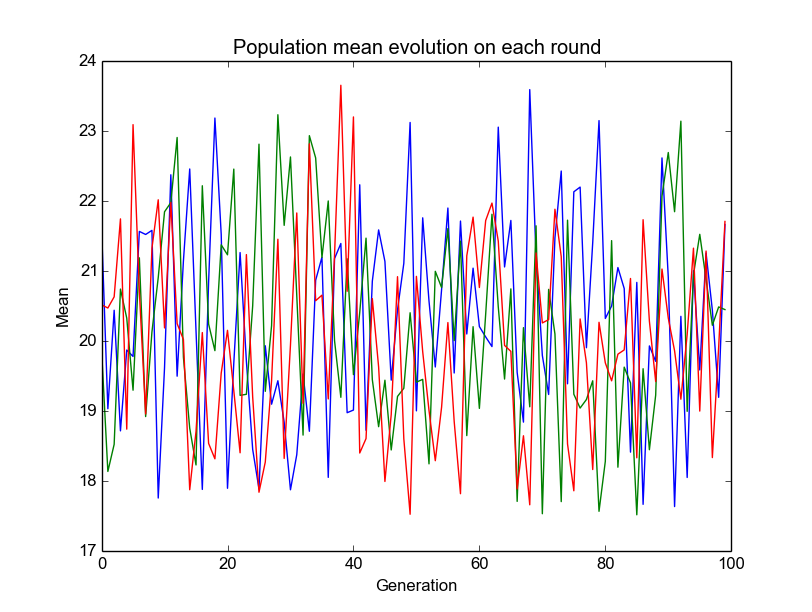
\includegraphics[scale=0.5]{QK_Means/img/bi_nofactor_mean.png}
% \caption{DB index mean of the population in T2. Only 4 rounds represented.}
% \label{fig:db_index_mean_t2}
% \end{figure}

% \begin{figure}[hbtp]
% \centering
% 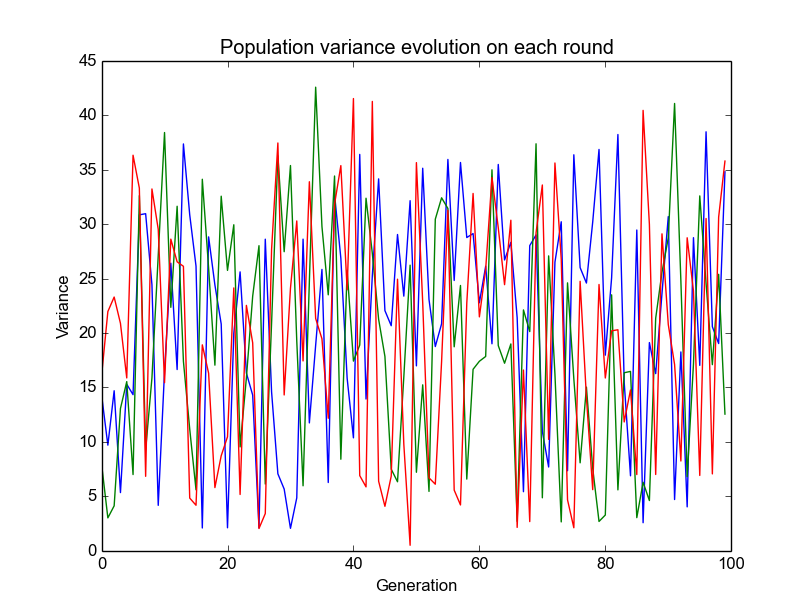
\includegraphics[scale=0.5]{QK_Means/img/bi_nofactor_var.png}
% \caption{DB index variance of the population in T2. Only 4 rounds represented.}
% \label{fig:db_index_var_t2}
% \end{figure}


% Analysing the evolution of the DB index of the best solution over the generations (Fig. \ref{fig:qk_db_index_best_evo_t2} and \ref{fig:qk_db_index_best_evo_t3}) gives some insight on the rate of convergence. In both tests it is clear that the best solution is often reached in a quarter of the total generations. More detail can be seen in the Table \ref{tab:db_index_t1_t3}.

% \begin{figure}[hbtp]
% \centering
% 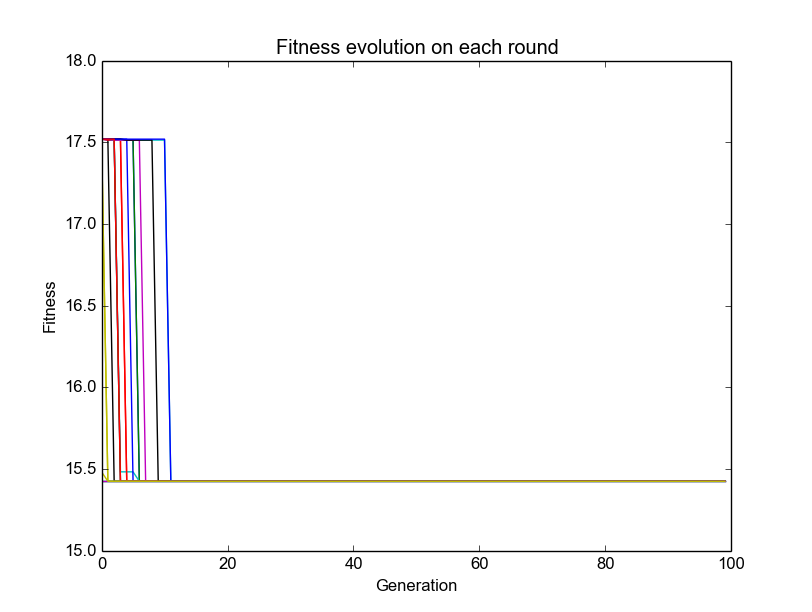
\includegraphics[scale=0.5]{QK_Means/img/bi_nofactor_evo.png}
% \caption{DB index of best solution in T2.}
% \label{fig:qk_db_index_best_evo_t2}
% \end{figure}


% \begin{figure}[hbtp]
% \centering
% 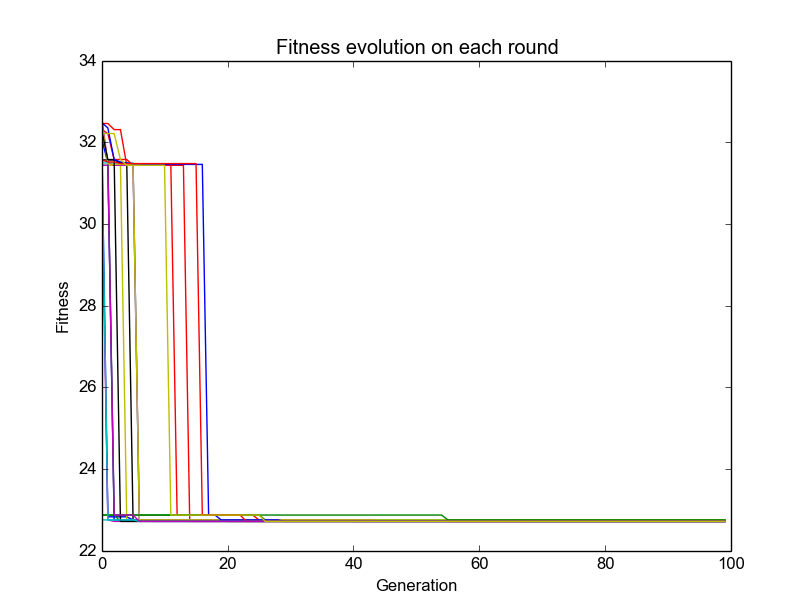
\includegraphics[scale=0.5]{QK_Means/img/sex_evo.png}
% \caption{DB index of best solution in T3.}
% \label{fig:qk_db_index_best_evo_t3}
% \end{figure}

% % table in csv format available in resource directory -->

% \begin{table}[h]
% \centering
% \caption{The values represent generations.}

% \begin{tabular}{lllll}

% \toprule
% \textbf{Test} & \textbf{Mean} & \textbf{Variance} & \textbf{Best} & \textbf{Worst} \\
% \midrule

% \textbf{T1}   & 17.25         & 70.2875           & 3             & 33             \\
% \textbf{T3}   & 28.05         & 568.6475          & 2             & 90             \\ 
% \bottomrule
% \end{tabular}

% \label{tab:db_index_t1_t3}
% \end{table}




\subsection{Horn and Gottlieb's algorithm}

For measuring the performance of Horn and Gottlieb's algorithm, several mixtures of 4 Gaussians with different number of patterns and dimensions were produced. %cardinality and dimensionality were produced.
Table \ref{tab:horn performance} presents the execution times for each of these datasets.
It can be seen that the execution time of this algorithm is rather high even for small datasets as the ones presented, since this algorithm is being analyzed with the goal of speed optimization.
More than 1 hour for a small dataset such as $10 \: 000$ patterns is prohibitive for application in the EAC context.

\begin{table}[h]
\centering
\caption{Time of computation of \citet{Horn2001b} algorithm for a mixture of 4 Gaussians of different cardinality and dimensionality.}

\begin{tabular}{rrr}
\toprule
 Cardinality &  Dimensionality &     Time [s] \\
\midrule
          10 &               2 &     0.035382 \\
          10 &               3 &     0.411391 \\
          10 &               4 &     0.385114 \\
          10 &               5 &     0.429747 \\
         100 &               2 &     2.954650 \\
         100 &               3 &     3.322593 \\
         100 &               4 &     3.743720 \\
         100 &               5 &     4.143823 \\
        1000 &               2 &    52.840666 \\
        1000 &               3 &    60.293262 \\
        1000 &               4 &    68.225671 \\
        1000 &               5 &    81.523212 \\
       10000 &               2 &  3009.678259 \\
       10000 &               3 &  3418.342830 \\
       10000 &               4 &  3956.289064 \\
       10000 &               5 &  4918.185844 \\
\bottomrule
\end{tabular}

\label{tab:horn performance}
\end{table}


In spite of its computational complexity, the accuracy of the algorithm was tested on the Iris and Crab datasets, taken from the UCI Machine Learning repository \cite{Lichman:2013}.
The Iris dataset has 150 patterns, 4 features and 3 classes where 2 are overlapping.
The Crab dataset has 200 patterns, 5 features and 4 classes where 2 pairs of classes are overlapping.
Principal Component Analysis (PCA) was applied to both datasets before clustering.
An accuracy as high as $86\%$ was obtained for the Iris dataset when using the first and second principal components (PC), and as high as $82\%$ when using all PCs.
For the Crab dataset an accuracy of $81.5\%$ was obtained for the second and third PCs (PCs chosen to reproduce the results of the original source of the algorithm), $63\%$ when using all PCs.
However, when applied to the unprocessed data the accuracy was only $34\%$ .


%TODO
%Put in accuracy results for crab,iris and gaussian mixtures  
%Put in timing results


% The accuracy of this algorithm was tested with real world datasets, namely, the crab and iris datasets available at the UCI Machine Learning Repository.

% %TODO add ref for repository -->

% \subsection{Iris data}
% \label{sec:horn_iris}
% The iris dataset ([available at the UCI ML repository](http://archive.ics.uci.edu/ml/datasets/Iris)) has 3 classes each with 50 data points. There are 4 features. The data is preprocessed using Principal Component Analysis (PCA). The natural clustering can be observed in Fig. \ref{fig:iris_natural}. 

% % #TODO saved image from ipython -->

% \begin{figure}[hbtp]
% \centering
% 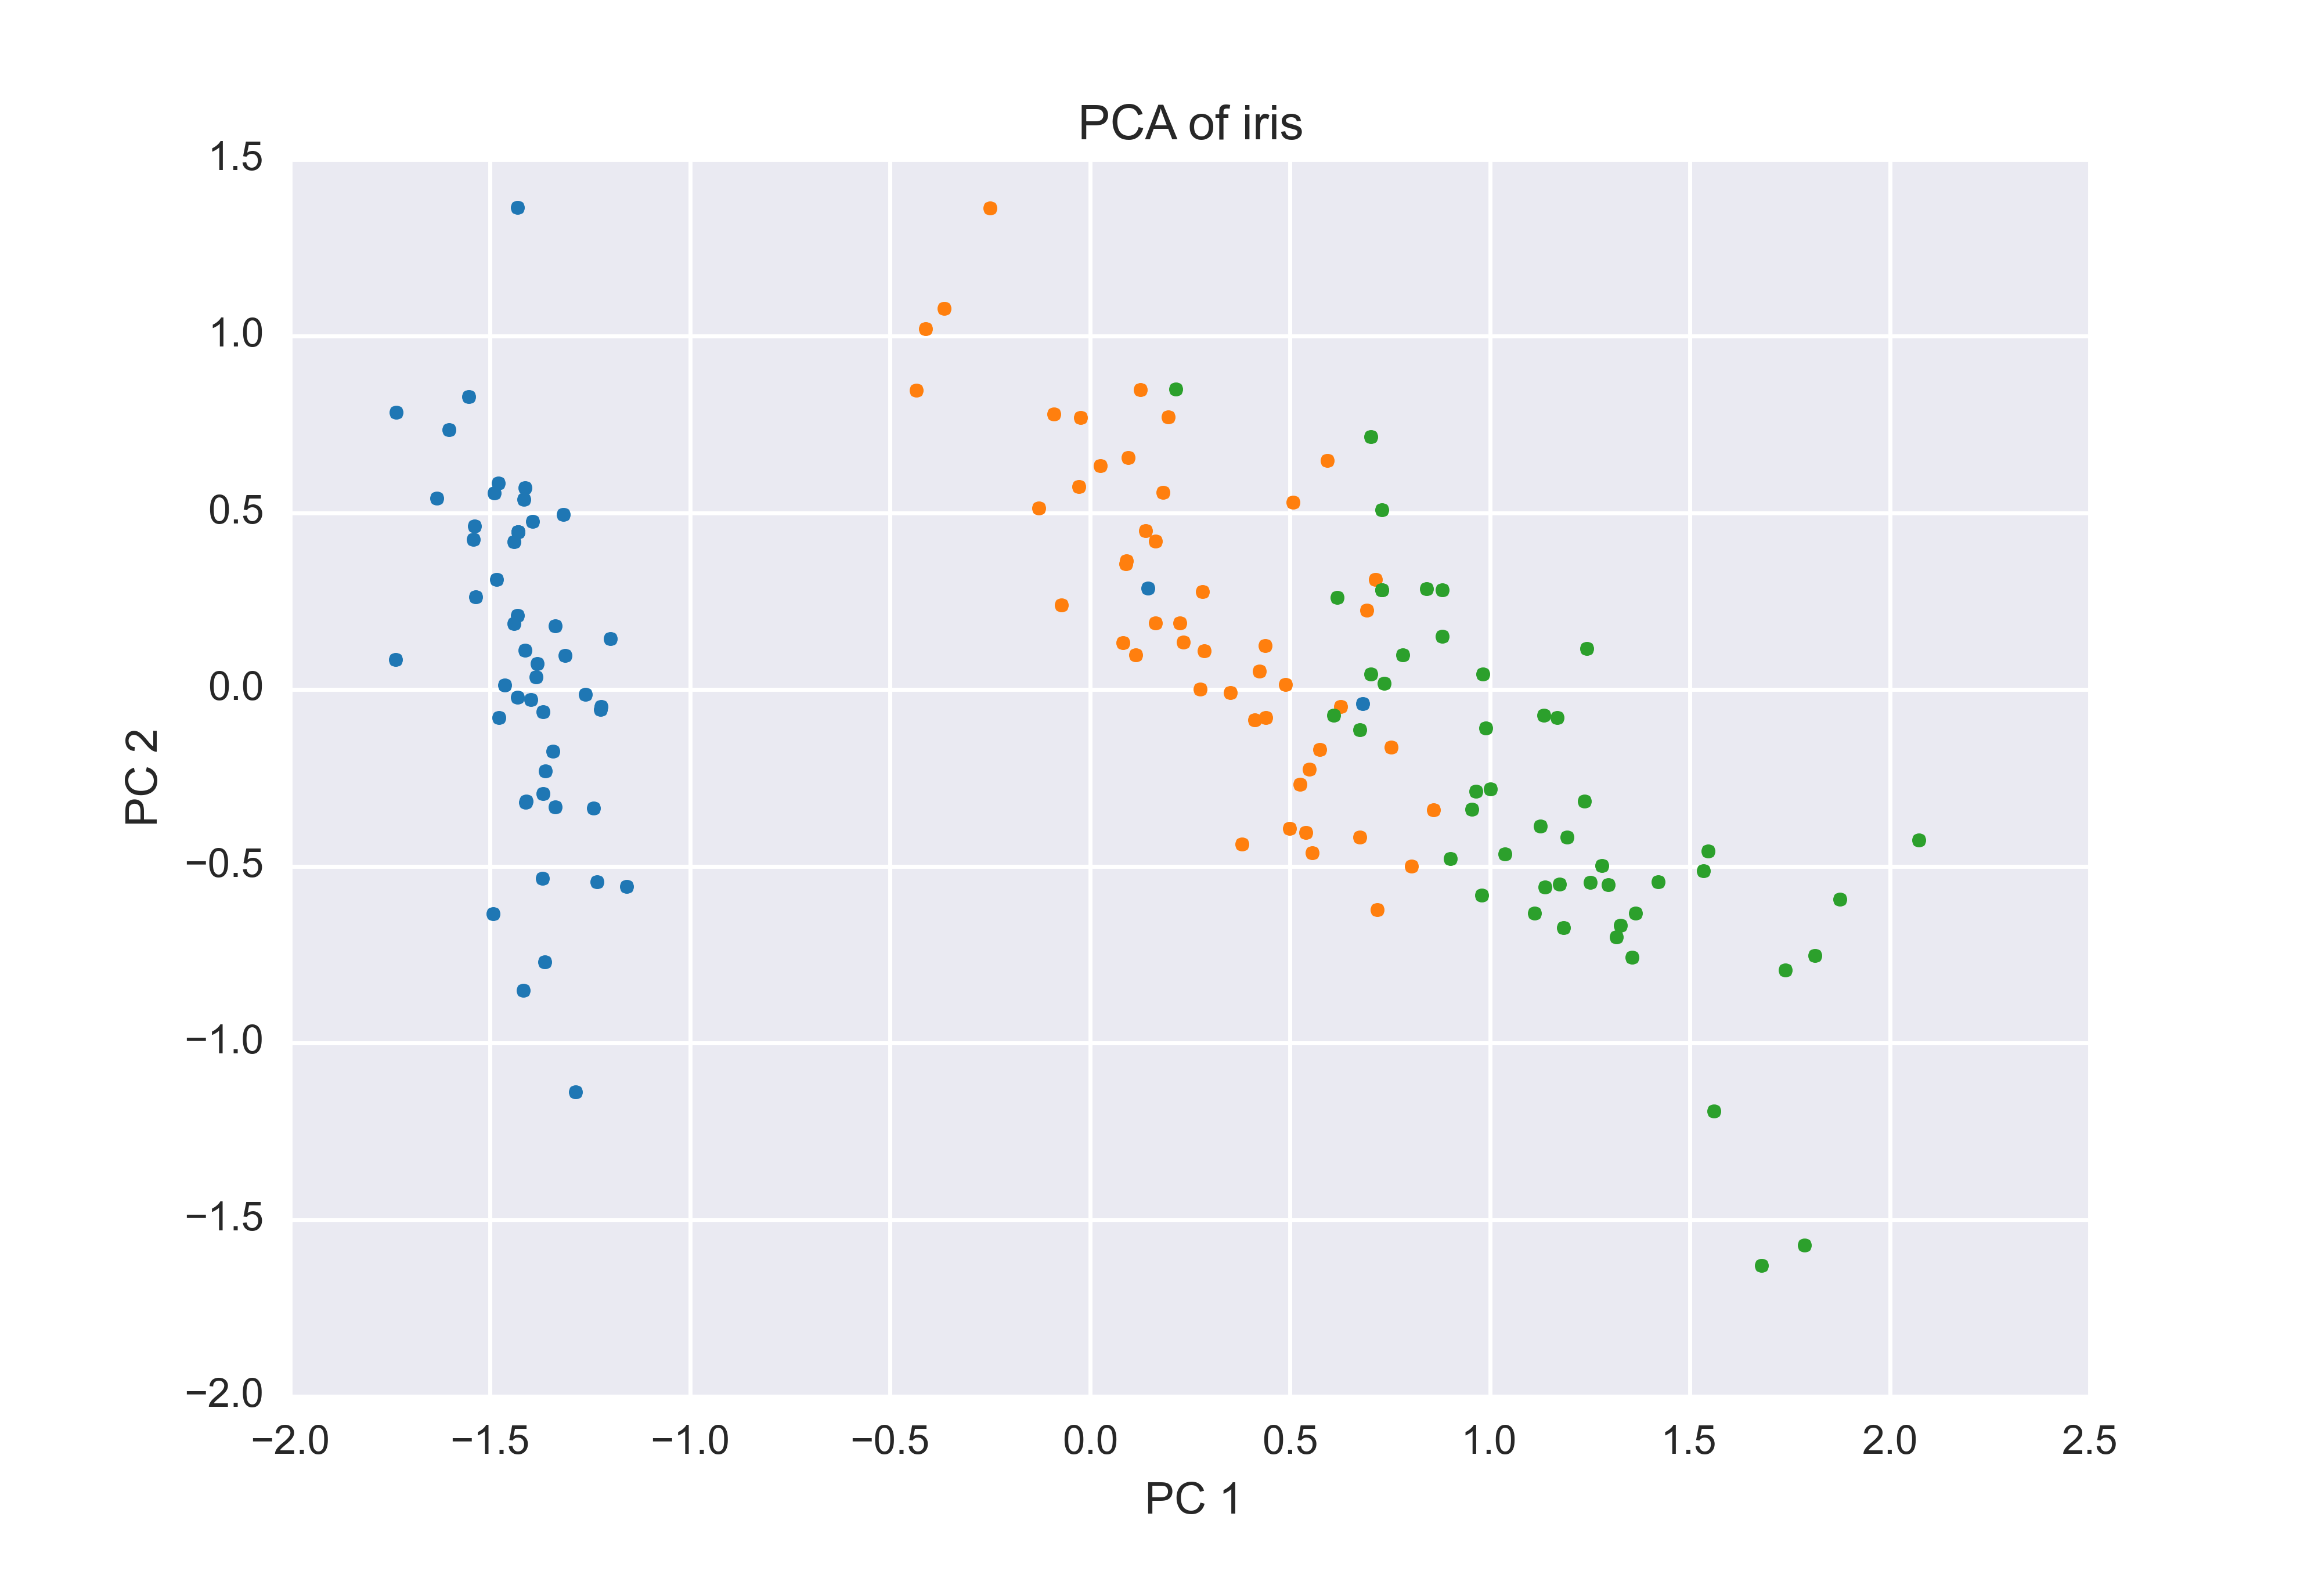
\includegraphics[scale=0.5]{Horn/img/iris_natural.png}
% \caption{Plot of the two first principal components (PC).}
% \label{fig:iris_natural}

% \end{figure}

% I chose $\sigma=\frac{1}{4}$ to reproduce the experiments in [3]. Only the first two PC are used here, which account for $95.8\%$ of the energy. The clustering results can be seen in Fig. \ref{fig:iris_2pc_cluster} and have an accuracy of 86\% computed with consistency index.


% \begin{figure}[hbtp]
% \centering
% 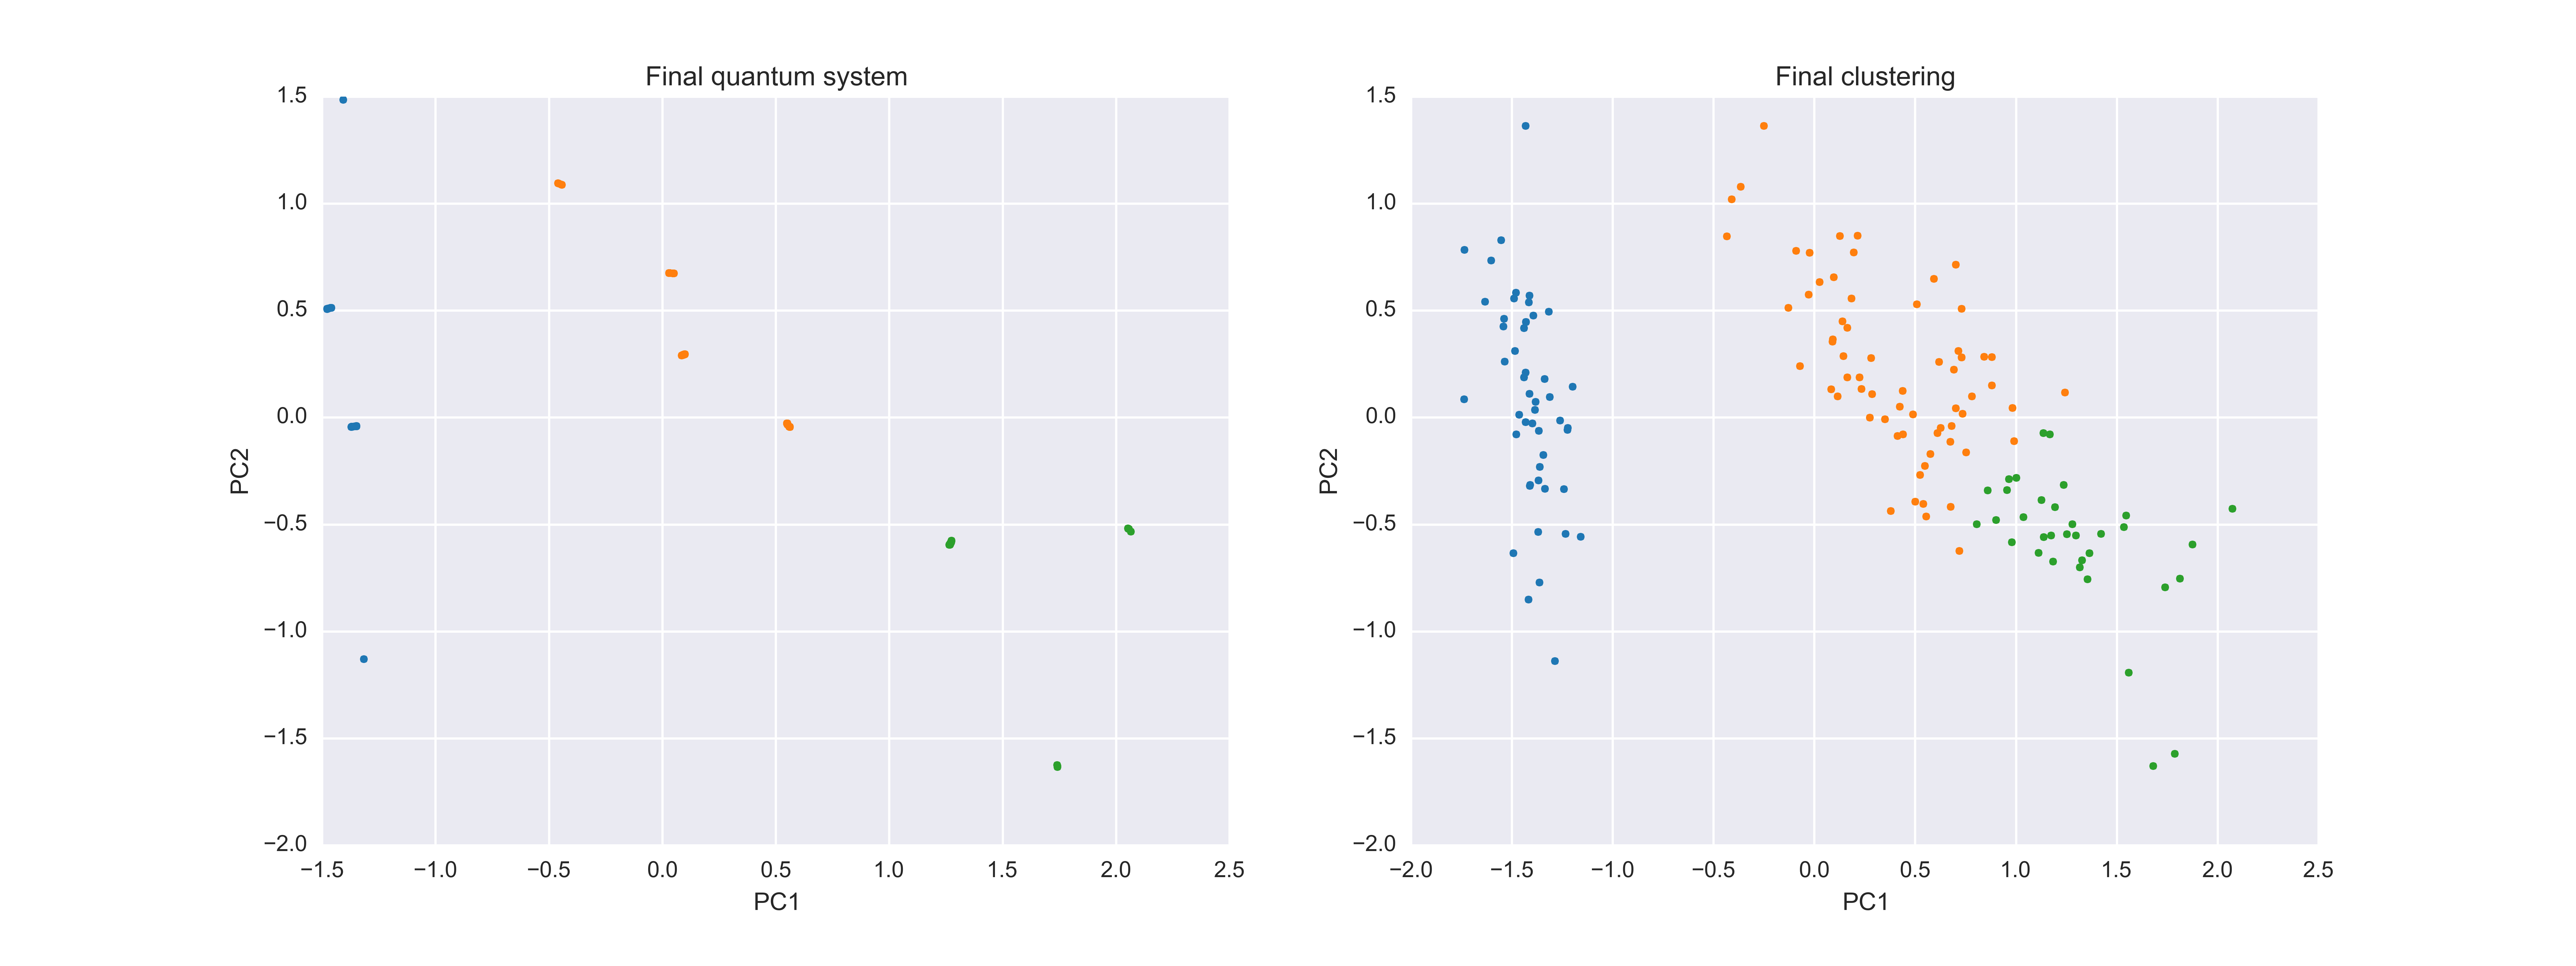
\includegraphics[width=\textwidth]{Horn/img/iris_2pc_cluster.png}
% \caption{Plots of the converged data data points and final clustering for 2 PC.}
% \label{fig:iris_2pc_cluster}

% \end{figure}

% For the sake of completeness, Fig. \ref{fig:iris_allpc_cluster} shows the clustering over all PCs. This solution has an accuracy of 82.67\% computed with consistency index.


% \begin{figure}[hbtp]
% \centering
% 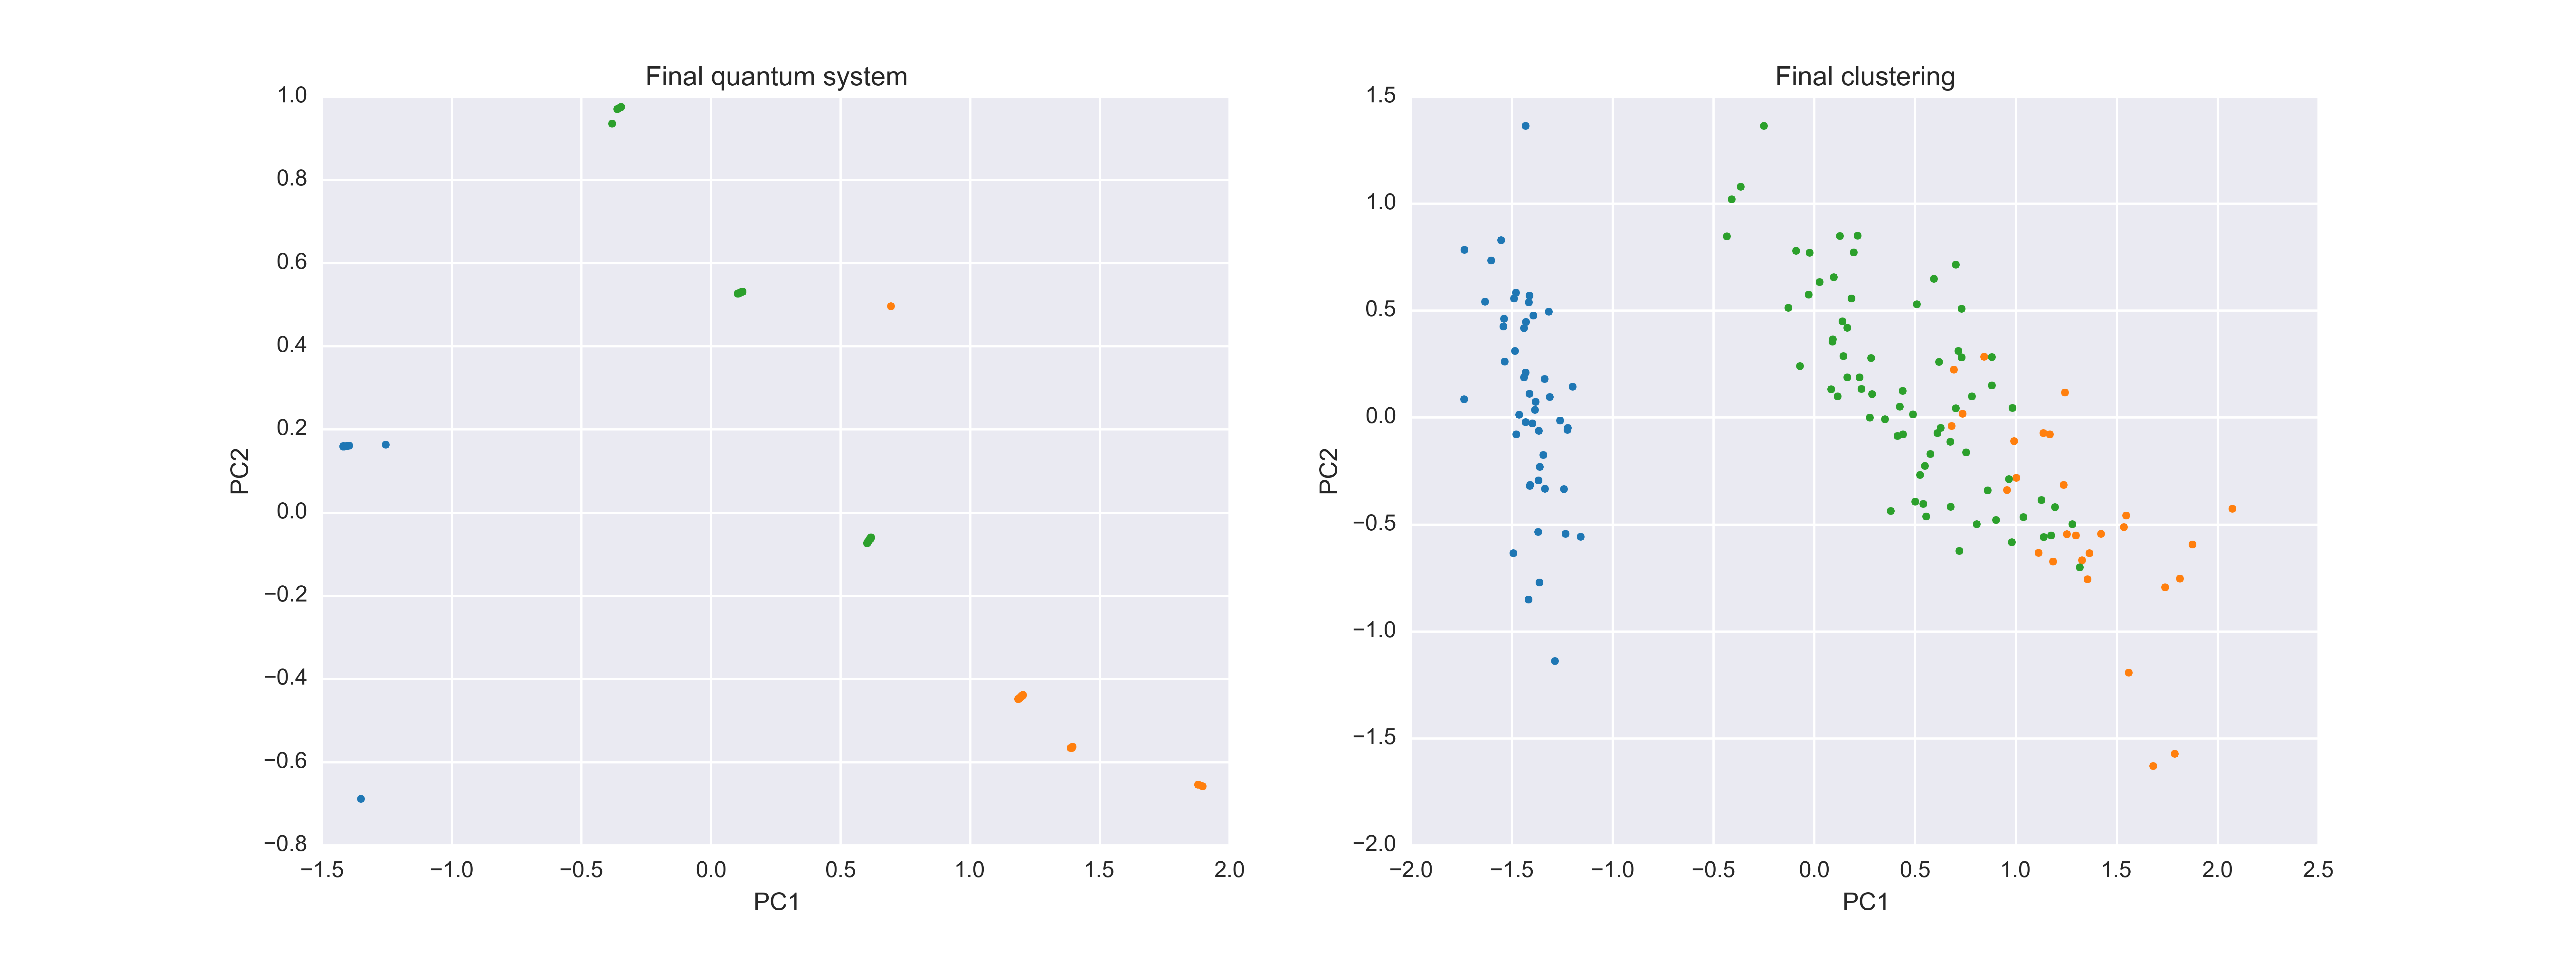
\includegraphics[width=\textwidth]{Horn/img/iris_allpc_cluster.png}
% \caption{Plots of the converged data data points and final clustering for all PC of Iris data.}
% \label{fig:iris_allpc_cluster}
% \end{figure}


% \subsection{Crab data}

% The crabs dataset has 200 samples and describes 5 morphological measurements on 50 crabs each of two colour forms and both sexes (total of 200 crabs), of the species Leptograpsus variegatus collected at Fremantle, Western Australia. After a preprocessing using PCA with covariance matrix and uncentred data, the dataset is represented in Fig. \ref{fig:crab_2pc_covar}.% #TODO add reference to dataset -->

% \begin{figure}[hbtp]
% \centering
% 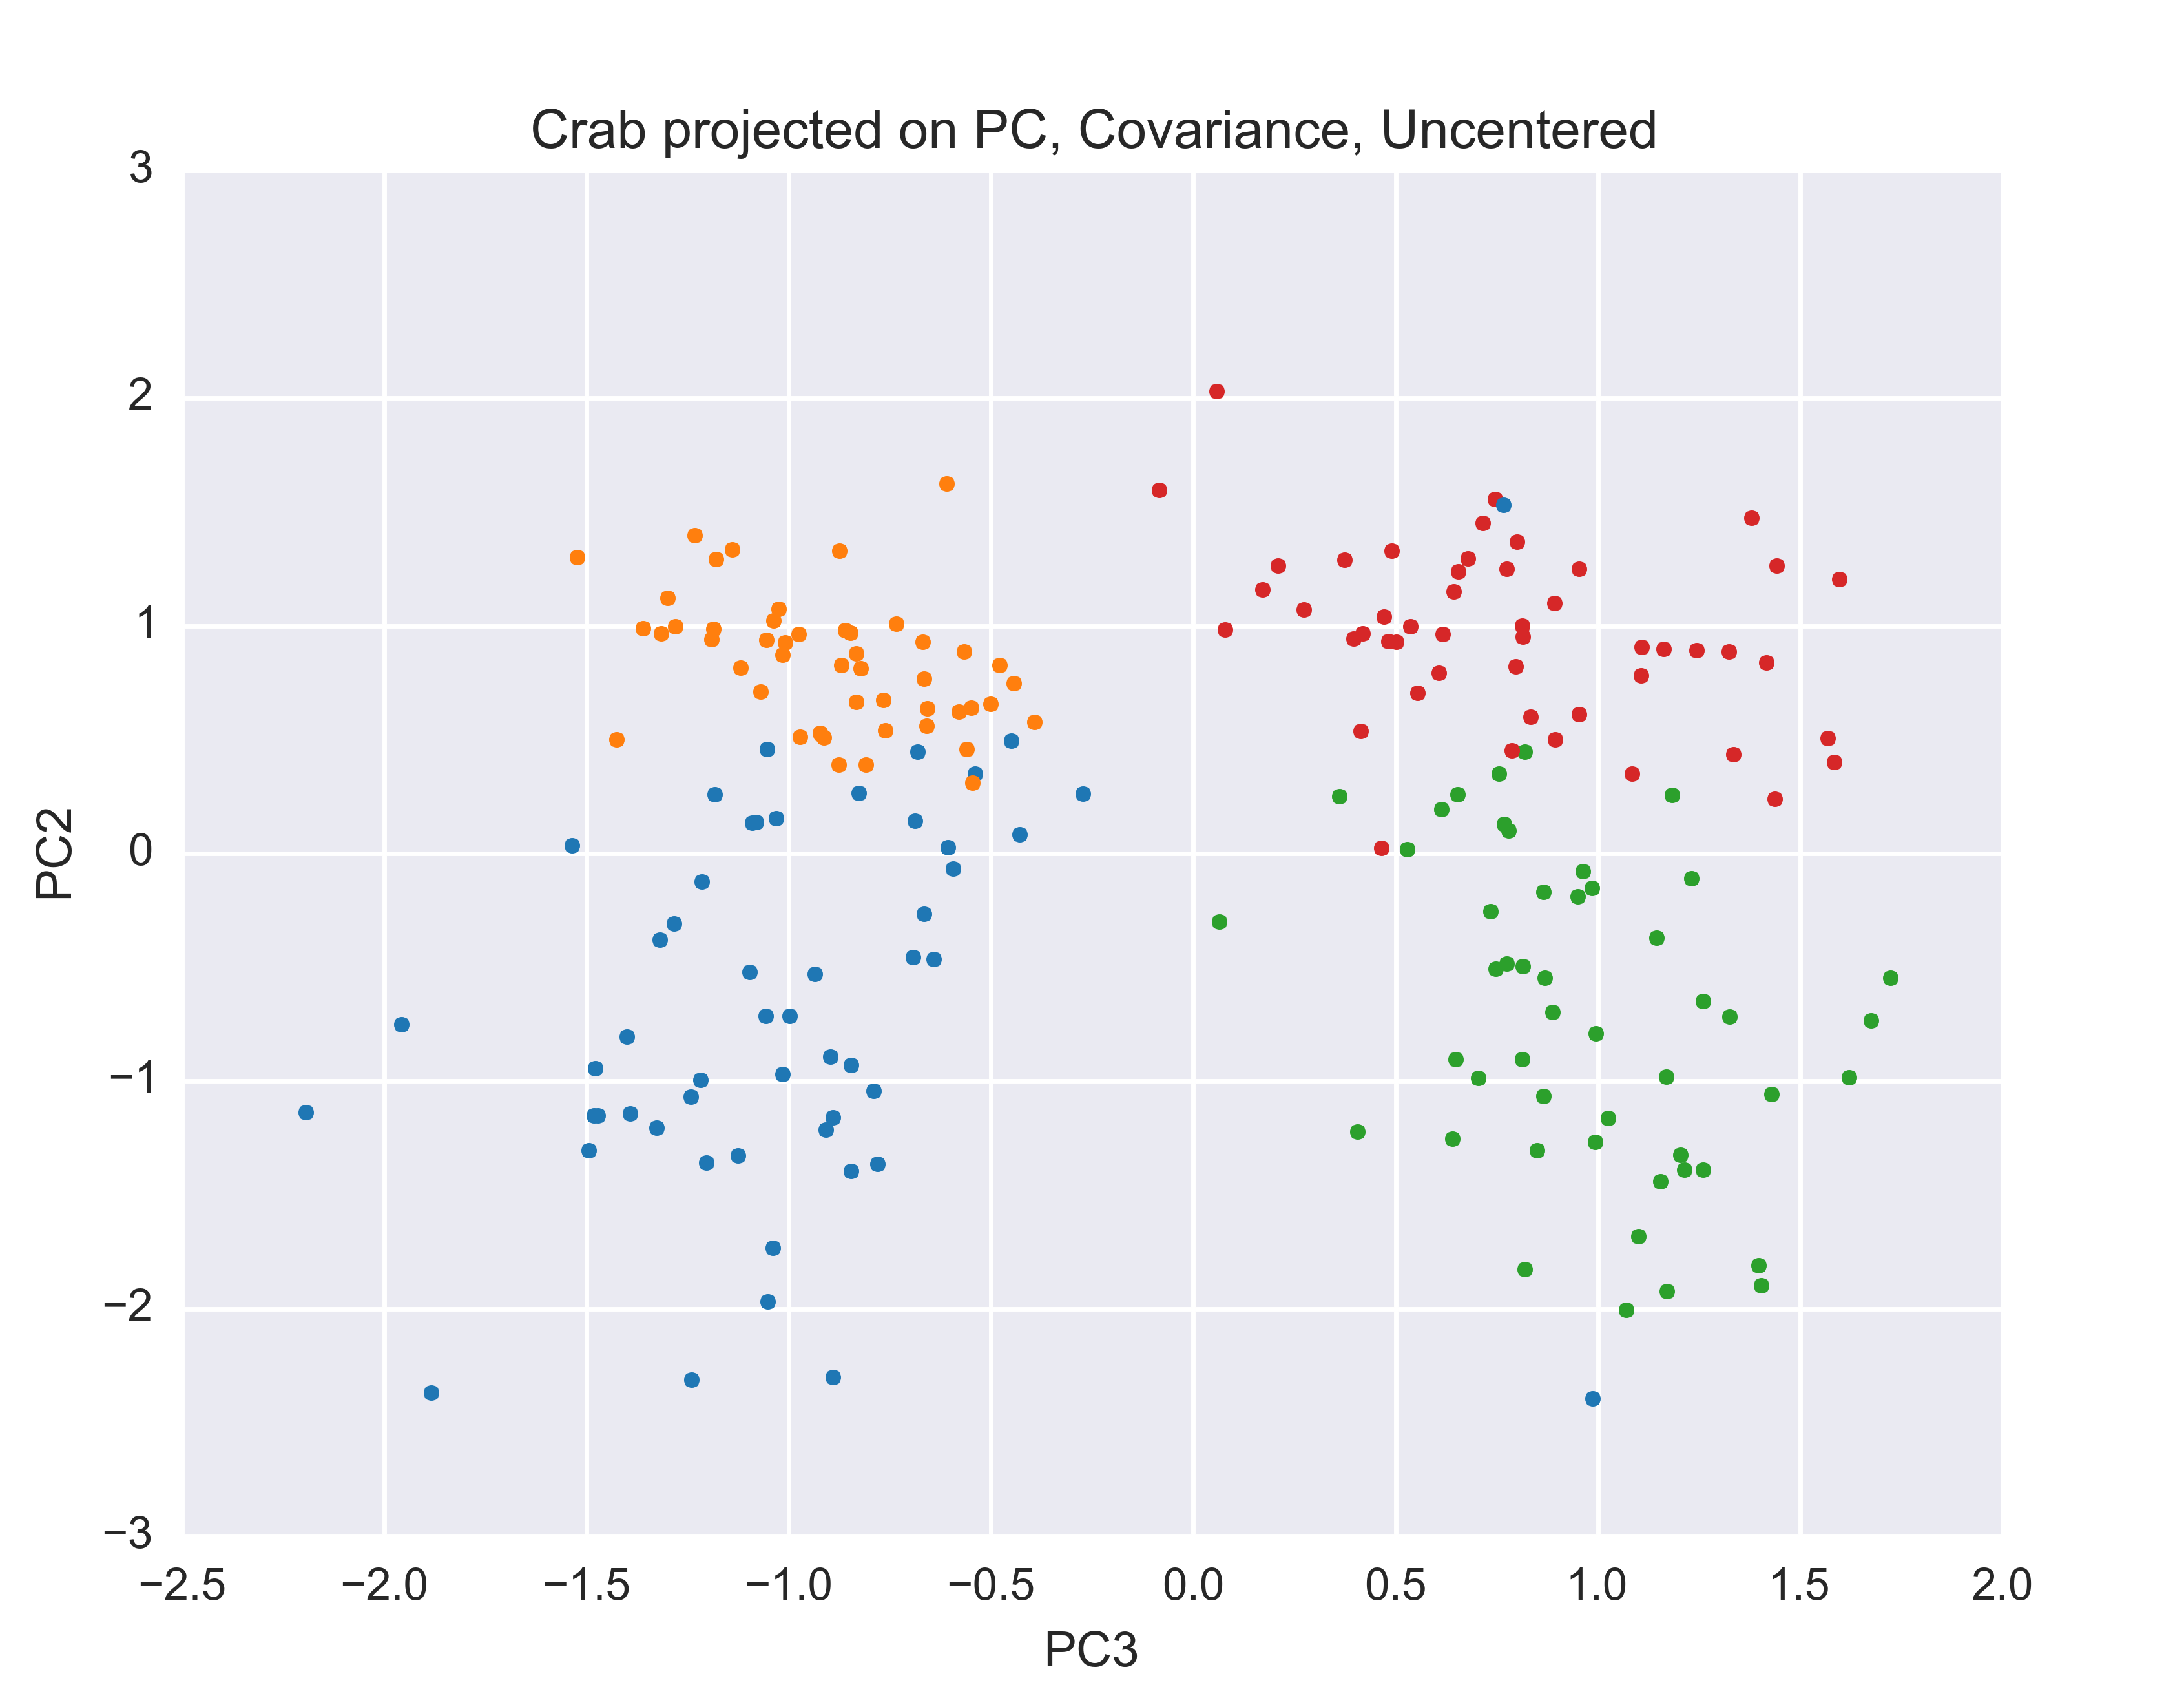
\includegraphics[scale=0.5]{Horn/img/crab_2pc_covar.png}
% \caption{Representation of the crab data projected over PC 2 and 3.}
% \label{fig:crab_2pc_covar}
% \end{figure}

% \begin{figure}[hbtp]
% \centering
% 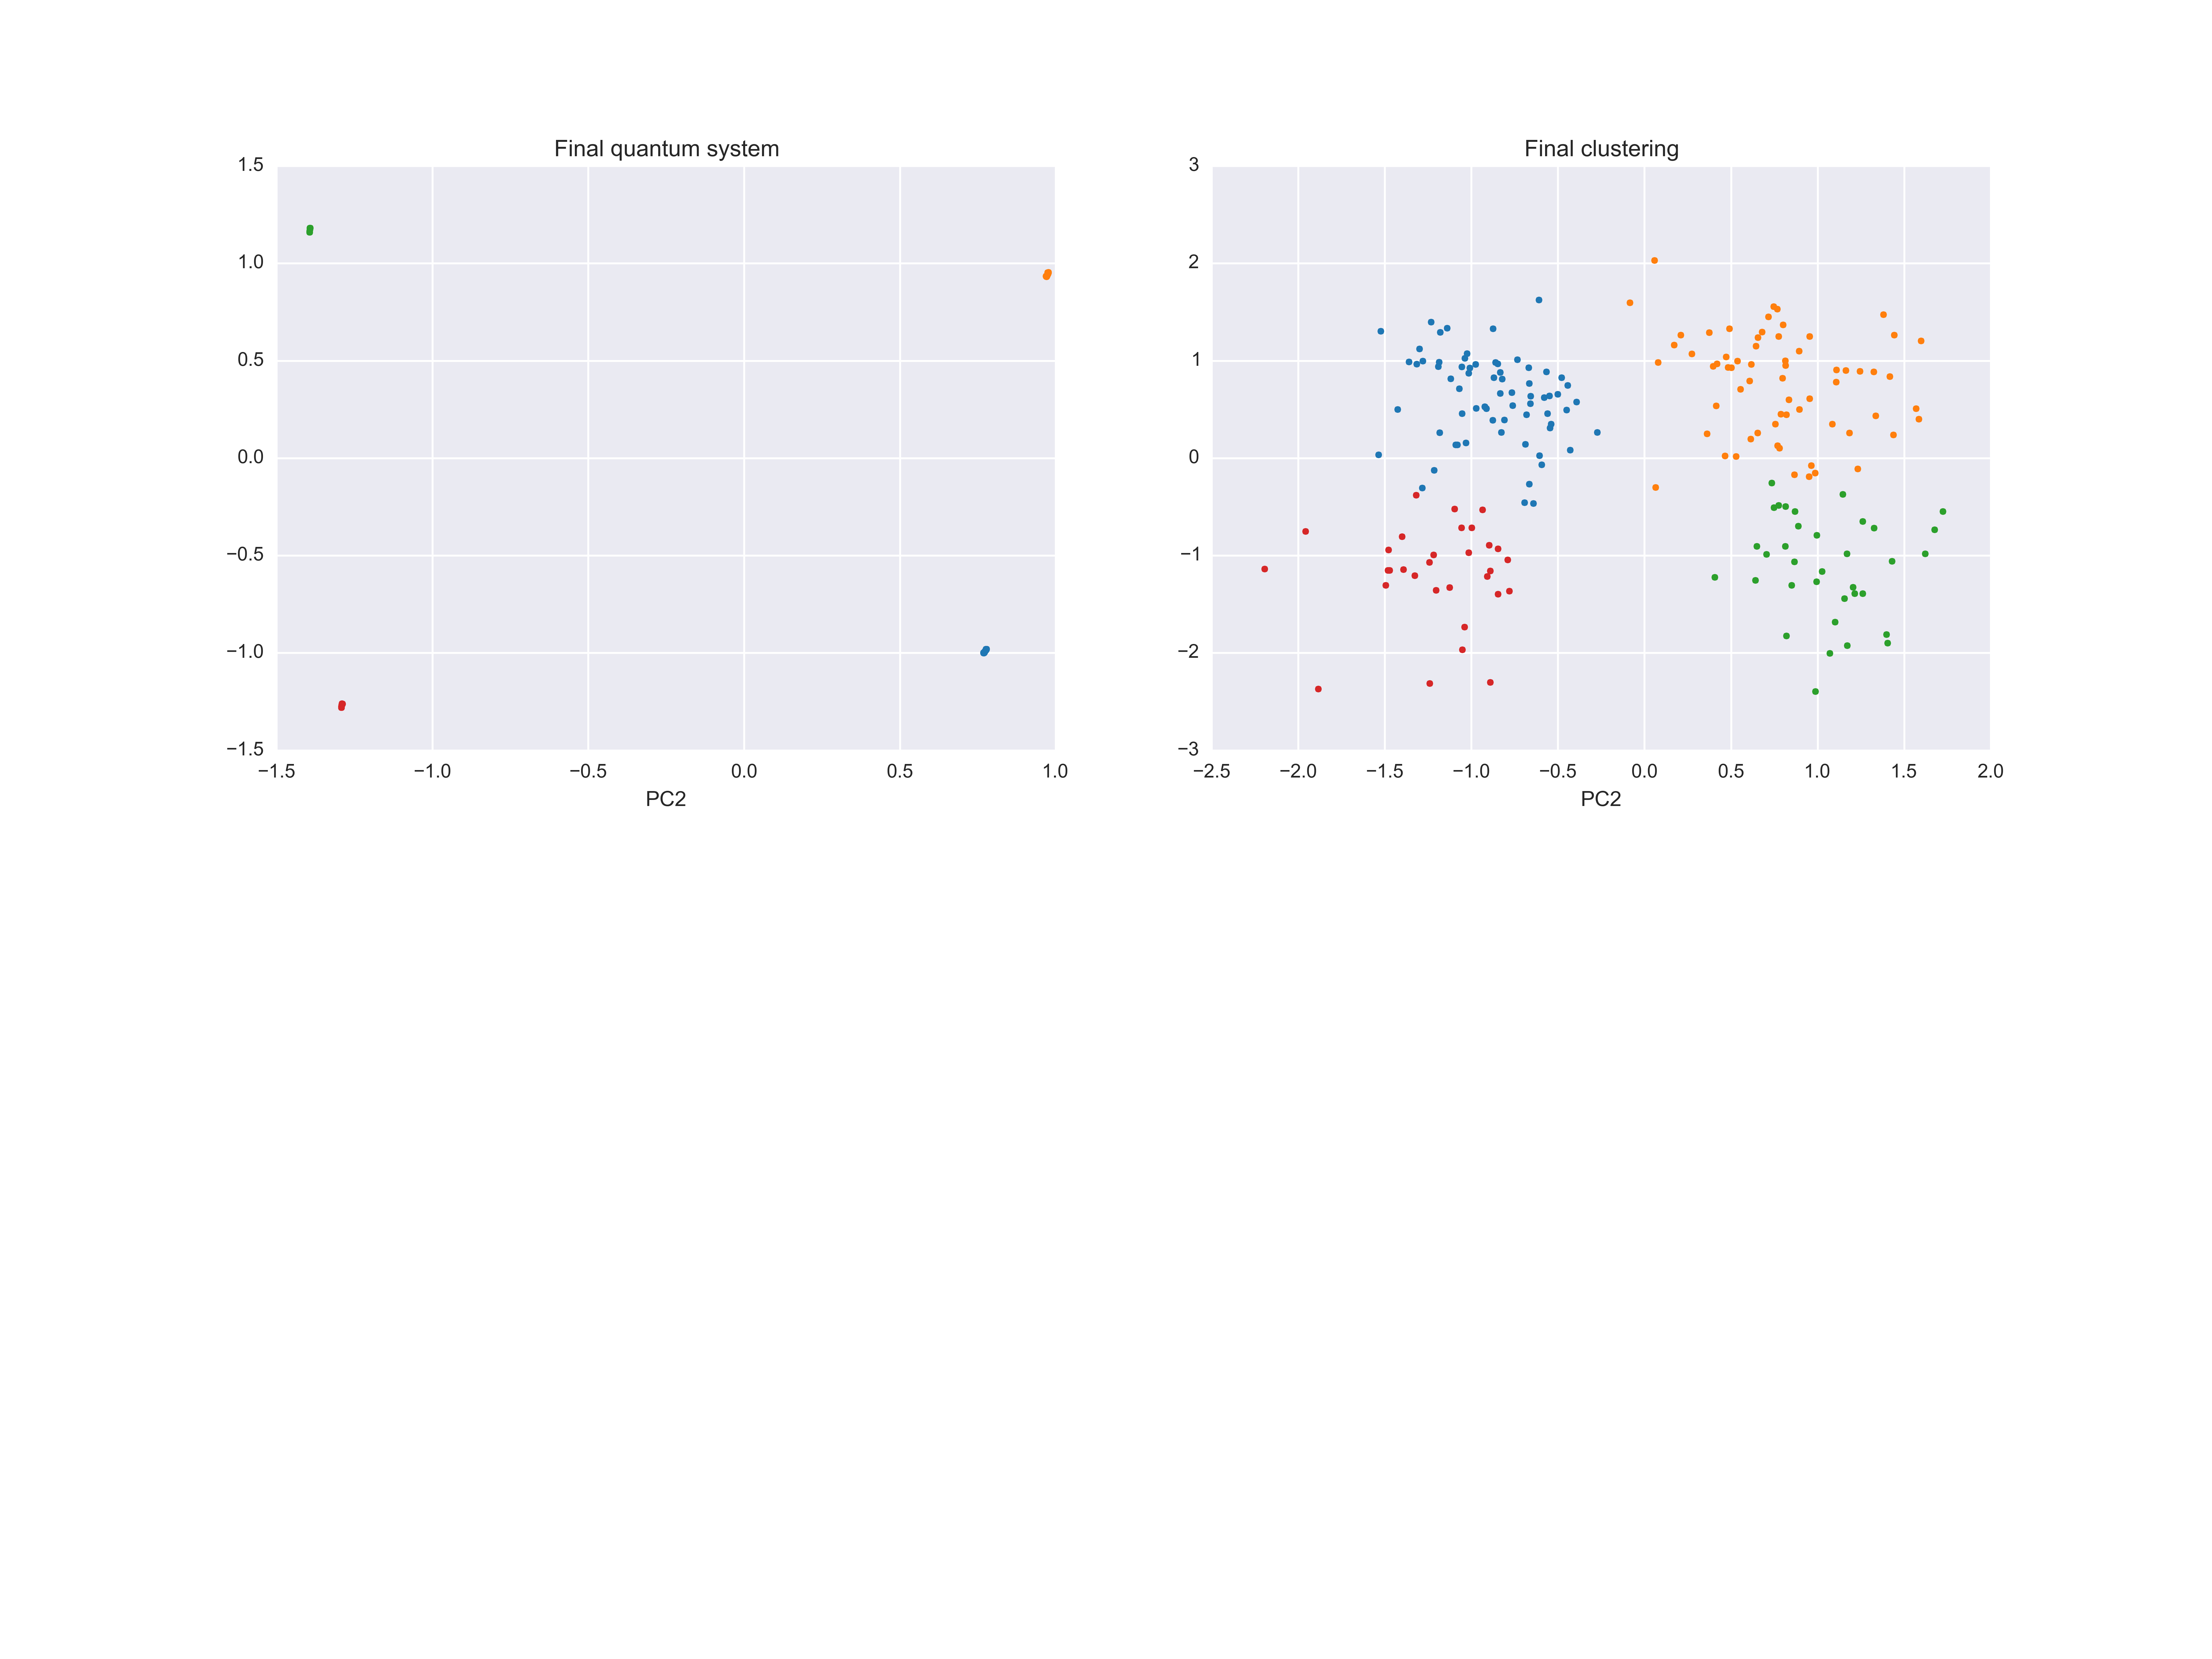
\includegraphics[width=\textwidth]{Horn/img/crab_2pc_covar_cluster.png}
% \caption{Representation of the crab data projected over PC 2 and 3.}
% \label{fig:crab_2pc_covar_cluster}
% \end{figure}

% \begin{figure}[hbtp]
% \centering
% \includegraphics[scale=0.5]{Horn/img/crab_2pc_covar_centered.png}
% \caption{Representation of the crab data projected over PC 2 and 3.}
% \label{fig:crab_2pc_covar_centered}
% \end{figure}

% \begin{figure}[hbtp]
% \centering
% \includegraphics[width=\textwidth]{Horn/img/crab_2pc_covar_centered_cluster.png}
% \caption{Representation of the crab data projected over PC 2 and 3.}
% \label{fig:crab_2pc_covar_centered_cluster}
% \end{figure}


% Initial work aimed at reproducing results from [2], but lack of detail on the preprocessing used made it an harder task. Several preprocessings were used, namely whitening or not the data, centring it or not, using covariance versus correlation and different methods of computing the PCs through eigenvalue decomposition or Singular Value Decomposition (SVD). The closest representation to that of the [2] is the one if Fig. C1.


% %TODO finish crab

% Covariance uncentred consistency index = 0.815
% Covariance centred consistency index = 0.91

% all pc covariance uncentred consistency index = 0.63
% all dimensions original data consistency index = 0.34 % QUANTUM RESULTS
\section{Parallel K-Means}
\label{sec:parallel kmeans}

This section will present results relevant to the GPU parallel K-Means.
Its purpose is to understand how dataset complexity (number of patterns, features and centroids) affect the speed-up of the GPU version over the CPU.
All tests were executed on machine Charlie and the block size was maintained constant at 512.

% \subsection{Maximum potential speed-up}

% Previously, it was mentioned that the methodology followed for speeding up an application was to first profile the code and identify the portions of code that can be optimized and what fraction of the total computational time they take.
% Table \ref{tab:kmeans max speedup} presents statistical results on the theoretical maximum speed-up for the two K-Means phases.
% The sequential version of K-Means was executed over a wide spectrum of datasets varying the number of patterns, dimensions and centroids. % cardinality, dimensionality and number of clusters.
% The theoretical maximum speed-up is considered to be the overall speed-up of the algorithm if one of its phases had infinite speed-up, i.e. when its time is negligible relative to the other phases.
% Analyzing these results it is clear that the labeling phase holds the most potential for optimizations.
% Furthermore, the theoretical speed-up also increases with the problem complexity (number of patterns, dimensions and centroids), since, the execution time for the labeling phase with more complex datasets is higher compared to the update phase.
% The theoretical speed-up of the update phase is almost negligible when compared to the labeling phase.
% This illustrates the importance of profiling the code before proceeding with optimizations, since effort invested in the update phase would yield little effect.

% \begin{table}[h]
% \centering
% \caption{Maximum theoretical speed-up for the labeling and update phases of K-Means based on experimental data. The datasets used range from $1000$ to $500 \: 000$ patterns, from $2$ to $1000$ dimensions and from $2$ to $2048$ centroids.}

% \begin{tabular}{lrr}
% \toprule
% {} &  Labeling phase &  Update phase \\
% \midrule
% mean  &               540.830750 &                    1.046810 \\
% std   &               879.914267 &                    0.083625 \\
% min   &                 2.998327 &                    1.000199 \\
% 25\% percentile &      18.657822 &                    1.001470 \\
% 50\% percentile &      99.868132 &                    1.010139 \\
% 75\% percentile &     681.250941 &                    1.056709 \\
% max   &              5026.972226 &                    1.519945 \\
% \bottomrule
% \end{tabular}

% \label{tab:kmeans max speedup}
% \end{table}


\subsection{Analysis of speed-up}

Observing Figures \ref{fig:kmeans dim 2} and \ref{fig:kmeans dim 200}, it is clear that the number of patterns, dimensions and centroids influence the speed-up.
It should be noted that whenever the number of centroids was superior to $70\%$ of the number of patterns, that particular test case was not executed.
For the simple case of 2 dimensions (Fig \ref{fig:kmeans dim 2}), the speed-up increases with the number of patterns.
However, there is no speed-up when the overall complexity of the datasets is low.
For 2 clusters, there is no speed-up before of $100 \: 000$ patterns.
And even after that mark, the speed-up is not significant relative to higher number of clusters.
The reason for this is that the benefits from the parallelization of such simple problems does not outweigh the cost of the memory transfers.
On the other hand, for a large number of clusters, there is speed-up for any number of patterns processed.
Not only that, that speed-up is highest of any other case with inferior number of clusters.
The reason for this is that the total amount of work increases linearly with the number of clusters but is diluted by the number of threads that can execute simultaneously.

\begin{figure}[hbtp]
    \centering
    \includegraphics[width=\textwidth]{{{results/kmeans/fixed_dimensions/2.0}}}
    \caption{Speed-up of the labeling phase for datasets of 2 dimensions and varying cardinality and number of clusters. The dotted black line represents a speed-up of one.}
    \label{fig:kmeans dim 2}
\end{figure}

However, as the number of dimensions increases (observe Fig. \ref{fig:kmeans dim 200}), the speed-up increases until a certain number of patterns and then decreases.
Here, the initial number of patterns for which there is a speed-up is lower than in the low dimensionality case and the number of clusters plays less an influence on the speed-up.
It is believed that the reason for this is related to the implementation itself.
The current parallel implementation does not use shared memory, which is fast.
As such, for every computation, each thread fetches the relevant data from global memory which is significantly slower.
As the number of dimensions increases, the amount of data that each thread must fetch also increases.
Furthermore, since the number of dimensions affects both data points and centroids, if the number of dimensions increases by 2 the number of fetches to memory increases by 4.
So, the speed-up increases with the dataset complexity until a point where the number of fetches to memory starts having a very significant effect on the execution time, decreasing the speed-up close to $50\%$.

% As it stands, this implementation of K-Means excels in low-dimensional datasets with a high number of centroids.
% Good performance on a high number of centroids is a desireble thing given the overall context 

\begin{figure}[hbtp]
    \centering
    \includegraphics[width=\textwidth]{{{results/kmeans/fixed_dimensions/200.0}}}
    \caption{Speed-up of the labeling phase for datasets of 200 dimensions and varying cardinality and number of clusters. The dotted black line represents a speed-up of one.}
    \label{fig:kmeans dim 200}
\end{figure}



\subsection{Effective bandwidth and computational throughput}
% check devblogs.nvidia.com/parallelforall/how-implement-performance-metrics-cuda-cc/

Effective bandwidth and throughput are two useful metrics to measure the efficiency of CUDA programs.
The effective bandwidth was computed by summing the times of transferring data to and fro the device divided by the total amount of data transfered and is usually represented in GBytes/s.
The computational throughput is usually represented in GFLOP/s (Giga-FLoating-point OPerations per second).
These metrics were computed from the results and a statistical overview is presented in Table \ref{tab:kmeans performance metrics}.
The results refer only to the labeling phase to make a fair comparison between CPU and GPU, although considering both phases would not alter significantly the results since the update phase represents a small fraction of the computational complexity.
The computational throughput of the GPU is more than 3 times higher than that of the CPU, on average.
However, it is interesting to note that the minimum GPU throughput is significantly lower than the CPU.
This is because of what was seen in previous sections, where the dataset complexity is too low for the overhead associated with using the GPU to outweigh the benefit of the parallel computation.
Furthermore, it should be noted that the effective metrics of the GPU are well below the maximum theoretical presented in the device specifications, which are a bandwidth of 288 GB/s and a throughput of 4.29 TFLOP/s.
This suggests that the GPU is underused on the presented test cases.
The same reason for the lower speed-ups on higher dimensional problems may explain the GPU underuse.

\begin{table}[ht]
\centering
\caption{Effective bandwidth and computational throughput of labeling phase computed from results taken from running K-Means over datasets whose complexity ranged from $100$ to $10 \: 000 \: 000$ patterns, from $2$ to $1000$ dimensions and from $2$ to $2048$ centroids.}

\begin{tabular}{lrrr}
\toprule
{} &  GPU bandwidth [GB/s] &  GPU throughput [GFLOP/s] &  CPU throughput [GFLOP/s] \\
\midrule
mean             &         2.90 &    3.65 &        1.04 \\
std              &         2.27 &    4.51 &        0.33 \\
min              &         0.00 &    0.00 &        0.02 \\
25\% percentile &          0.56 &    1.54 &        0.87 \\
50\% percentile  &         2.89 &    1.71 &        1.17 \\
75\% percentile  &         5.31 &    4.16 &        1.29 \\
max             &          6.04 &   21.91 &        1.44 \\
\bottomrule
\end{tabular}

\label{tab:kmeans performance metrics}
\end{table}

\subsection{Influence of the number of points per thread}

The number of patterns each thread processes (PPT) may influence performance as well.
To evaluate this hypothesis, several runs over the datasets of $500 \: 000$ patterns with different points per thread were executed.
A brief statistical analysis of the results is presented in Table \ref{tab:kmeans cuda ppt}.
The average speed-up almost doubled when executing 2 PPT.
For more than 2 PPT, the speed-up seemed to decrease with an increase of the number of PPT.
Since the labeling kernel was not optimized for reducing the number of memory calls when processing more than one PTT, the increase in speed-up may be justified by the reduced overhead of calling less blocks of threads.
The fraction of the threads that did not execute any patterns increased with the PPT, which may be the cause for the decrease of speed-up with an increase of PPT after 2.

\begin{table}[h]
\centering
\caption{Speed-up obtained in the labeling phase for different number of patterns per thread (PPT).}


\begin{tabular}{lrrrrr}
\toprule
{} &       {} 	   &   {} 		   &  \textbf{Speed-up}  & {} 		& {}\\
{} &       PPT = 1 &       PPT = 2 &       PPT = 4 &       PPT = 8 &      PPT = 16 \\
\midrule
mean  			 &   5.9 &  10.1 &   3.7 &   3.1 &   2.1 \\
std   			 &   7.5 &  13.4 &   4.0 &   3.0 &   1.3 \\
min   			 &   1.2 &   2.4 &   1.5 &   1.4 &   1.3 \\
25\% percentile  &   1.3 &   2.6 &   1.6 &   1.5 &   1.4 \\
50\% percentile  &   2.0 &   2.7 &   1.7 &   1.6 &   1.4 \\
75\% percentile  &   4.8 &   9.4 &   2.1 &   1.9 &   1.7 \\
max   			 &  24.2 &  46.7 &  12.8 &   9.9 &   4.9 \\
\bottomrule
\end{tabular}

\label{tab:kmeans cuda ppt}
\end{table} % KMEANS RESULTS
\section{Building the co-association matrix with different sparse formats}
\label{sec:spare building}

The purpose of this section is to present brief results concerning the time that took to build a co-association matrix for different types of matrices.
The ensemble from which the co-association matrices are built has 100 partitions and was produced from a mixture of 6 Gaussians with 5000 patterns.
Only the upper triangular (condensed) matrix was built.
The types of matrices under test are: fully allocated (a "normal" matrix), LIL, DOK, CSR, an optimized fully allocated and the proposed EAC CSR.
The SciPy's LIL, DOK and CSR implementations were used.
All tests were executed in machine Bravo.

The time that took to update the first partition and the total time were recorded for the different types of matrix.
The results are presented in Table \ref{tab:coassoc build sparse} and also in Fig. \ref{fig:coassoc build sparse}.
For the CSR format only the first partition was updated, since it took a very long time to update just the first partition.
A rough estimate for the time it would take to update the whole matrix is around 15 hours, 100 times the time it took to update the first partition.
Observing the other timings, and for the exception of the EAC CSR matrix, this estimate should not be too far off.
The reason that the first partition update of the EAC CSR matrix was so much faster is that it only requires a simple copy of the partition to the data structure.

It is clear from the results that the optimized versions are much faster than any of the others.
These results focus on providing a justification for the design and implementation of a novel method of building the co-association matrix: a fully allocated matrix consumes too much memory but available sparse implementations are too slow.
For this purpose a small dataset as the one used suffices to demonstrate this point.
The difference between the two optimized versions will become clearer on future sections, where a more thorough study covering a wider spectrum of datasets is presented. 


\begin{table}[h]
\centering
 \caption{Execution times for computing the condensed co-association matrix using different matrix strategies.}
\begin{tabular}{crr}
\toprule
  Matrix type (condensed) &  Time 1st partition [s] &  Time ensemble [s] \\
\midrule
 Optimzed Fully allocated &                 0.001 &              0.139 \\
                  EAC CSR &                 0.004 &              1.470 \\
          Fully allocated &                 0.855 &             96.000 \\
                      LIL &                 5.390 &            614.000 \\
                      DOK &                12.500 &           1535.000 \\
                      CSR &               548.000 &                - \\
\bottomrule
\end{tabular}
\label{tab:coassoc build sparse}
\end{table}



\begin{figure}[hbtp]
\centering
\includegraphics[scale=0.6]{results/eac_sparse_build/coassoc_build_bar}
\caption{Execution times for computing the condensed co-association matrix using different matrix strategies.}
\label{fig:coassoc build sparse}
\end{figure} % SPARSE BUILDNG RESUTLS
%!TEX root = Thesis.tex
\section{GPU MST}
\label{sec:gpu mst}

% From Sousa dissertation - the graphs he used and where he took them from
% The graph collection supplied provided by 9th DIMACS Implementation Challeng \footnote{http://www.dis.uniroma1.it/~challenge9/} include sparse graphs
% that depict the United States road network. These graphs are seen frequently in the recent literature. Furthermore, the OpenStreetMap’s \footnote{http://www.openstreetmap.org/} Portuguese road-network, provided by Geofabrik \footnote{http://download.geofabrik.de/europe/portugal.html} is included.

To test the performance of the GPU MST algorithm, several graphs were used.
Most of the graphs are United Stated road network graphs taken from the 9th DIMACS Implementation Challenge \footnote{http://www.dis.uniroma1.it/~challenge9/}, the same used in the original source \cite{Sousa2015}.
Furthermore, graphs taken from the co-association matrix of the second step of EAC were used.
This is important because, as will become clear, the graphs within the EAC paradigm have different characteristics.
All the tests were performed on machine Bravo.
The average speed-up obtained by using the GPU version over the sequential one is presented in Table \ref{tab:mst speedup}.
Characteristics of the different graphs are also shown so as to illustrate what variables influence the speed-up obtained.
It should be noted that a speed-up below 1 is actually a slow-down.

\begin{minipage}[h]{\hsize}
	\centering
	\captionof{table}{Average speed-up of the GPU MST algorithm for different data sets, sorted by number of edges.}
\begin{tabular}{lrrrrr}
\toprule
Data set &  No. vertices &   No. edges &     Speed-up \footnote{Average speed-up from 10 rounds of executing the algorithm on each graph.} &  No. edges / vertex & Memory [MBytes]\\
\midrule

NY                           &      264347 &    730100 &  0.77 &          2.76 &    7.59 \\
BAY                          &      321271 &    794830 &  0.79 &          2.47 &    8.52 \\
COL                          &      435667 &   1042400 &  0.99 &          2.39 &   11.28 \\
FLA                          &     1070377 &   2687902 &  1.39 &          2.51 &   28.67 \\
NW                           &     1207946 &   2820774 &  1.45 &          2.34 &   30.74 \\
NE                           &     1524454 &   3868020 &  1.56 &          2.54 &   41.14 \\
CAL                          &     1890816 &   4630444 &  1.58 &          2.45 &   49.75 \\
LKS                          &     2758120 &   6794808 &  1.69 &          2.46 &   72.88 \\
E                            &     3598624 &   8708058 &  1.80 &          2.42 &   93.89 \\
W                            &     6262105 &  15000000 &  1.94 &          2.39 &  163.13 \\
Coassoc 50k \footnote{Co-association matrix of a 100 partition ensemble produced from a mixture of 6 Gaussians with $50 \: 000$ patterns, using the rule sk=sqrt\_2 th=30\%.} 							   &       50000 &  30296070 &  0.20 &        605.92 &  231.52 \\
CTR                          &    14000000 &  34000000 &  2.09 &          2.43 &  365.82 \\

\bottomrule
\end{tabular}
\label{tab:mst speedup}
\end{minipage}

% note on the memory usage
Although all the graphs presented in Table \ref{tab:mst speedup} occupy significantly less memory than available in the used machine, the processing of bigger graphs is not possible.
The reason for this is that between each iteration two graphs have to be held in memory: the initial and the contracted.
Moreover, the space occupied by the contracted graph will depend on the characteristics of the graph.

% speed-ups are possible, contrast with original paper
The results clearly show that it is possible to obtain speed-ups for computing a MST.
This speed-up seems to increase with the size of the graph, with the notable exception of the graph from the EAC context.
A note should be made here to bring to attention the contrast between these results and those presented by \citet{Sousa2015}.
The speed-ups observed here are less than those reported by \citet{Sousa2015}.
This is believed to be related with the technology stack used and this topic has been discussed in more depth in chapter \ref{chapter:methodology}.
To understand how different parameters affect the speed-up of the algorithm, Table \ref{tab:mst corr} presents the correlation matrix of these variables.

\begin{table}[h]
\centering
 \caption{Cross-correlation between several characteristics of the graphs and the average speed-up.}
\begin{tabular}{lrrr}
\toprule
{} &  No. vertices &   No. edges &        No. edges / vertex \\
\midrule
Average speed-up             &    0.692 &  0.081 &         -0.654 \\
\bottomrule
\label{tab:mst corr}
\end{tabular}
\end{table}

%TODO run MST algorithm with more graphs of different characteristics
% what are the variables that influence speed-up
The row corresponding to the average speed-up is of special relevance.
One can observe that the parameters most correlated with the speed-up are the number of vertices and the number of edges per vertex (EPV).
The correlation matrix suggests that as one increases the number of vertices, the speed-up will also increase.
In fact, if no graphs from the EAC context were present in the results, the same would apply to the number of edges, since the EPV would be very similar.
The reason for this is that speed-ups from parallelism are more salient when applied to big datasets, so that the speed-up of the computation itself outweighs the overhead associated with communication between host and device.
The EPV is the other parameter that shows has highest (inverse) correlation with the speed-up.
This suggests that the relationship between the number of edges and the number of vertices in the graph actually plays a big role in deciding if there will be a speed-up.
In essence, this expresses the sparsity of the graph and results manifested speed-ups only for very sparse graphs.

% why, programatically, there is slow-down
The underlying reason for the poor performance of graphs with high EPV ratio is believed to be that, since the parallel computation is anchored to vertices, the workload per vertex is higher than if the graph had a low ratio.
Accordingly, the workload per vertex is higher from the beginning and can increase significantly as the algorithm progresses.
Besides, the workload can become highly unbalanced with some threads having to process hundreds of thousands of edges while others only a few thousands, which translates threads not doing any computation when waiting for the others.

% connection with original paper
The original source \cite{Sousa2015} of the algorithm doesn't address graphs with a EPV as high as presented here.
In that sense, the results here complement those of the original source and suggest an increase in EPV translates in a decrease in speed-up.
Still, this serves as motivation for more in-depth studies.

% connection with EAC
Within EAC paradigm, this algorithm is of little contribution for scaling to large datasets.
The most obvious reason is that the EAC method would actually be slower if this algorithm was used.
Still, even considering that speed-ups like those reported in literature were possible for EAC co-association graphs, the algorithm requires a double redundancy of edges (which effectively doubles the necessary memory to hold a graph) and at any iteration the device must be able to hold two distinct graphs (the initial and the contracted).
For these reasons, the device memory (which typically is smaller than the host memory) would confine the EAC method to small input datasets. 

% The underlying reason for this is believed to be that the number of edges to node ratio of these graphs is low compared to that typically seen in co-associations matrix, even when using a prototype subset of the original matrix.
% The parallel version of the final step of EAC showed a slowdown relative to its sequential counterpart.
% This slowdown is related with the performance of the MST algorithm.
% The implementation of the algorithm was tested in some of the same graphs as those reported in \cite{Sousa2015} and revealed a speedup.
% However, when using the this MST solver on the target graphs (the co-association matrices) not only there was no speedup, but a significantly slowdown was observed, reaching up to nine times slower.
 % GPU MST RESULTS
\section{EAC Validation}
\label{sec:eac validation}

The present section aims to provide results showing that the proposed methods do not alter the overall quality of the results.
With this in mind, the results of the original version of EAC, implemented in Matlab, are compared with those of the proposed solution.
Several small datasets, chosen from the datasets used by \citet{Lourenco2010} and taken from the UCI Machine Learning repository \cite{Lichman:2013}, were processed by the two versions of EAC.
Furthermore, since the generation of the ensemble is probabilistic and can change the results between runs, the proposed version is processed with the ensembles created by the original version as well.
This guarantees that the combination and recovery phases of EAC, which are deterministic when using SL, are equivalent to the original.
All data in this section refers to processing done in machine Alpha.

Table \ref{tab:validation error acc} presents the difference between the accuracies of the two versions.
Analyzing these results, it is apparent that the difference is minimal.
It should be noted at this point that the original implementation always maps the dissimilarities of the co-association matrix to the range $\left [ 0 , 1 \right ]$.
This forces the co-association matrix to have a floating point data type.
However, since the number of partitions used is usually less than 255, the proposed version uses unsigned integers of 1 byte to reduce the used memory considerably.
The differences in accuracy are thought to come from possible rounding differences and different implementations of core operations between Matlab and Python.

\begin{table}[h]
\centering
\caption{Difference between accuracies from the two implementations of EAC, using the same ensemble. Accuracy was measured using the H-index.}

\begin{tabular}{lll}
\toprule
         &        \multicolumn{2}{c}{Difference between accuracies of implementations} \\
dataset &      True number of clusters & Lifetime criteria \\
\midrule
breast\_cancer &  4.94e-06 &     2.82e-06 \\
ionosphere     &  1.65e-06 &      1.45e-06 \\
iris           &  3.33e-06 &      3.33e-06 \\
isolet         &  1.03e-07 &      4.08e-07 \\
optdigits      &  3.79e-06 &      1.48e-06 \\
pima           &  3.33e-06 &      3.33e-06 \\
pima\_norm     &  4.16e-07 &      4.16e-07 \\
wine\_norm     &  1.12e-07 &      1.91e-06 \\
\bottomrule
\end{tabular}

\label{tab:validation error acc}
\end{table}





% \begin{table}[h]
% \centering
% \caption{Speed-ups obtained in the combination and recovery phases of EAC, using the ensemble generated from the original EAC implementation.}

% \begin{tabular}{lll}
% \toprule
% dataset & Combination & Recovery \\
% \midrule
% breast\_cancer &   7.713564 &        15.22334 \\
% ionosphere    &   9.678288 &        20.12336 \\
% iris          &   14.25549 &         28.4751 \\
% isolet        &   5.500147 &        174.4283 \\
% optdigits     &   9.783604 &        53.21466 \\
% pima          &   85.21744 &        8.406726 \\
% pima\_norm     &   127.2274 &        12.89474 \\
% wine\_norm     &     8.0178 &        12.98206 \\
% \bottomrule
% \end{tabular}

% \label{tab:validation speedup comb rec}
% \end{table}

Table \ref{tab:validation speedup all} presents the speed-up of the proposed version over the original one.
It is clear that speed-up is obtained in all phases of EAC, often by an order of magnitude.
This result, combined with the demonstration that the differences in accuracy are negligible, show that the proposed algorithm performs well in small datasets.

\begin{table}[h]
\centering
\caption{Speed-ups obtained in the different phases of EAC, with independent production of ensembles.}

\begin{tabular}{lccrrrr}
\toprule
dataset &  No. patterns &  No. features & No. classes & Production & Combination & Recovery \\
\midrule
breast\_cancer &           683 &            10 &           2 &      50.4 &    7.5 &        15.8 \\
ionosphere     &           351 &            34 &           2 &      21.9 &   11.3 &        19.9 \\
iris           &           150 &             4 &           3 &      19.8 &   14.5 &        28.5 \\
isolet         &          7797 &           617 &          26 &       7.0 &    6.2 &       206.3 \\
optdigits      &          3823 &            64 &          10 &      17.3 &   10.2 &        53.0 \\
pima           &           768 &             8 &           2 &      50.7 &  141.5 &        13.9 \\
pima\_norm     &           768 &             8 &           2 &      54.3 &  132.9 &        14.4 \\
wine\_norm     &           178 &             4 &           3 &      22.9 &   14.6 &        25.3 \\
\bottomrule
\end{tabular}

\label{tab:validation speedup all}
\end{table}


 % EAC VALIDATION RESUTLS
\section{EAC}
\label{sec:eac results}

This section will present thorough results concerning several characteristics related to the EAC method.
These were the timings of the different parts, how the number of patterns and the different $K_{min}$ rules affected the sparsity of the co-association matrix, the typical number of associations per cluster in each rule, the growth of the number of associations with the different parameters, among others.
Two 2-dimensional 10 million pattern mixtures of 6 Gaussians were generated.
A variation of the number of dimensions has more interest in the performance characteristics of the production phase.
Since the production of the ensemble uses K-Means, detailed results can be found in section \ref{sec:parallel kmeans}.
One mixture has overlapping Gaussians and the other has not.
% The reasoning was that overlapping Gaussians might result in more associations per cluster.
The results contained in this section refer to the dataset with overlapping Gaussians, but the same overall patterns can be found in the other and the same conclusions can be drawn.

Different rules for computing the $K_{min}$, different co-association matrix formats and different approaches for the final clustering will be mentioned.
The different rules and their aliases are presented in Table \ref{tab:eac rules}.
The different formats for the co-association matrix are the \emph{full} (for fully allocated $n \times n$ matrix), \emph{full condensed} (for a fully allocated $\frac{n(n-1)}{2}$ array to build the upper triangular matrix), \emph{sparse complete} (for EAC CSR), \emph{sparse condensed const} (for EAC CSR building only the upper triangular matrix) and \emph{sparse condensed linear} (for EAC CSR condensed).
The different approaches for the final clustering are \emph{SLINK} \cite{Sibson1973}, \emph{SL-MST} (for using the Kruskal implementation in SciPy) and \emph{SL-MST-Disk} for the modified version that performs an external memory sort.

\begin{table}[h]
\centering
\caption{Different rules for computing $K_{min}$ and $K_{max}$. $n$ is the number of patterns and $sk$ is the number of patterns per cluster.}

\begin{tabular}{lcc}
\toprule
Rule &  $K_{min}$ &  $K_{max}$ \\
\midrule
\emph{sqrt}     & $\frac{\sqrt{n}}{2}$      & $\sqrt{n}$    \\
\emph{2sqrt}    & $\sqrt{n}$                & $2 \sqrt{n}$  \\
\emph{sk=sqrt2} & $sk = \frac{\sqrt{n}}{2}$ & $1.3 K_{min}$ \\
\emph{sk=300}   & $sk = 300$                & $1.3 K_{min}$ \\
\bottomrule
\end{tabular}

\label{tab:eac rules}
\end{table}

The experiment that generated the results of these section was set up as follows.
A large dataset was generated.
The dataset was sampled uniformly to produce a smaller dataset with the desired number of patterns.
A clustering ensemble was produced (production phase) for each of these smaller datasets and for each of the rules, using K-Means.
From each ensemble, co-association matrices of every applicable format were built (combination phase).
A matrix format was not applicable when the dataset complexity would make its correspondent co-association matrix too big to fit in main memory.
The final clustering (recovery phase) was also done for each of the matrix formats.
SLINK was used with fully allocated formats and the MST-based SL (SL-MST) and MST-based SL on external memory (SL-MST-disk) were executed with sparse matrices.
SL-MST was not executed if its space complexity was too big to fit in main memory.
Furthermore, the combination and recovery phases were repeated several times for smaller datasets for statistical relevant of the execution times, so as to make the influence of any background process less salient.
For big datasets, the execution times are big enough that the influence of background processes is negligible.

All results presented here originated from machine Bravo.

\subsection{Performance of production and combination phases}

The $K_{min}$ parameter, whose evolution is presented in Fig. \ref{fig:eac kmin evo}, influences several other EAC properties.
Rules \emph{sqrt}, \emph{2sqrt} and \emph{sk=sqrt2} never intersect with the increase if the number of patterns, but rule $sk=300$ intersects the others, finishing with the highest $K_{min}$.

\begin{figure}[hbt!]
    \centering
    \includegraphics[width=0.6\textwidth]{{{results/eac/kmin_evolution}}}
    \caption{Evolution of $K_{min}$ with cardinality for different rules.}
    \label{fig:eac kmin evo}
\end{figure}

The execution times for the production and combination phase can be observed in Figures \ref{fig:eac ensemble times}, \ref{fig:eac build rules} and \ref{fig:eac build matrices}, which allow the comparison between the different rules and the different matrix formats, respectively.
To avoid redundancy, only one matrix format is depicted to compare the execution times for the different rules and only one rule to compare the matrix formats.
The results of the other cases follow the same pattern.
Observing Fig. \ref{fig:eac build rules}, one can see the tendency of the evolution of$K_{min}$ in the production execution time associated with the $sk=300$ rule and the inverse in the combination time.
A higher $K_{min}$ means more centroids for K-Means to compute, so it is not surprising that the execution time for computing the ensemble increases as $K_{min}$ increases.
On the other hand, a higher $K_{min}$ translates in more condensed clusters and less associations per pattern.
With less associations, the computation time for building the co-association matrix naturally decreases.

\begin{figure}[hbt!]
    \centering
    \includegraphics[width=0.6\textwidth]{{{results/eac/ensemble_time}}}
    \caption{Execution time for the production of the clustering ensemble.}
    \label{fig:eac ensemble times}
\end{figure}

\begin{figure}[hbt!]
    \centering
    \includegraphics[width=0.6\textwidth]{{{results/eac/build_time/sparse_condensed_linear}}}
    \caption{Execution time for building the co-association matrix from ensemble with different rules.}
    \label{fig:eac build rules}
\end{figure}

In a previous section, the execution times for the combination phase had already been briefly presented when comparing different sparse formats.
Fig. \ref{fig:eac build matrices} shows the execution times on a longitudinal study for optimized matrix formats.
It is clear that the sparse formats are significantly slower than the fully allocated ones, specially for smaller datasets.
The \emph{full condensed} format usually takes close to half the time than the \emph{full} format, which is natural given that it performs half the operations.
Idem for the \emph{sparse condensed} formats compared to the \emph{sparse complete}.
The big discrepancy between the sparse and full formats is due to the fact that the former needs to do a binary search at each association update and needs to keep the internal sparse data structure sorted.


\begin{figure}[hbt!]
    \centering
    \includegraphics[width=0.6\textwidth]{{{results/eac/build_time/2sqrt}}}
    \caption{Execution time for building the co-association matrix with different matrix formats.}
    \label{fig:eac build matrices}
\end{figure}

\subsection{Performance comparison between SLINK, SL-MST and SL-MST-Disk}

The clustering times of the different methods of SL discussed previously (SLINK, SL-MST and SL-MST-Disk) are presented in Figures \ref{fig:eac sl}, \ref{fig:eac slink} and \ref{fig:eac sl-mst}.
The SL-MST-Disk method is significantly slower than any of the other methods.
This is expected, since it uses the hard drive which has very slow access times compared to main memory.
SL-MST is faster than SLINK, since it processes zero associations while SL-MST takes advantage of a graph representation and only processes the non-zero associations.
In resemblance to what happened with combination times, the condensed variants take roughly half the time has their complete counterparts.
This is expected, since SL-MST and SL-MST-Disk over condensed co-association matrices only process half the number of associations.
SLINK takes roughly the same time for every rule, which means $K_{min}$ has no influence, since SLINK processes the entire co-association matrix and $K_{min}$ only influences the number of non-zero associations.
The same rationale can be applied to SL-MST, where different rules can have significant influence over execution time, since they change the total number of associations.
As with the combination phase, the execution time referent to the \emph{sk=300} rule started with the greatest time and decreased with an increase in cardinality until it was the fastest.

\begin{figure}[hbt!]
    \centering
    \includegraphics[width=0.6\textwidth]{{{results/eac/sl_time/slink_vs_sl-mst}}}
    \caption{Comparison between the execution times of the three methods of SL. SLINK runs over fully allocated condensed matrix while SL-MST and SL-MST-Disk run over the condensed and complete sparse matrices.}
    \label{fig:eac sl}
\end{figure}

\begin{figure}[hbt!]
    \centering
    \includegraphics[width=0.6\textwidth]{{{results/eac/sl_mem_time/full_condensed}}}
    \caption{Comparison between the execution times of SLINK to different rules.}
    \label{fig:eac slink}
\end{figure}

\begin{figure}[hbt!]
    \centering
    \includegraphics[width=0.66\textwidth]{{{results/eac/sl_mem_time/sparse_condensed_linear}}}
    \caption{Comparison between the execution times of SL-MST for different rules.}
    \label{fig:eac sl-mst}
\end{figure}

\subsection{Performance of all phases combined}

The execution times of all phases combined are presented in Figures \ref{fig:eac total mem} and \ref{fig:eac total disk}.
The results are presented for the \emph{sparse condensed linear} format but the remaining results follow the same tendency.
It is interesting to note that, when using the SL-MST method in the recovery phase, the execution time for three of the rules do not differ much for large datasets.
This is due to a sort of balancing between a slowing down of the production phase and a speeding up of the combination and recovery phases as the $K_{min}$ increases at a higher rate for $sk=300$ than for other rules.
This is not observed for the $sqrt$ rule as $K_{min}$ is always low enough that the total time is always dominated by the combination and recovery phases.
The same does not happen when using the SL-MST-Disk method, as the total time is completely dominated by the recovery phase.
This is clear, since the results in Fig. \ref{fig:eac total disk} follow a pattern similar to that presented in Fig. \ref{fig:eac sl-mst}.


\begin{figure}[hbt!]
    \centering
    \includegraphics[width=0.6\textwidth]{{{results/eac/total_time_sl-mst}}}
    \caption{Execution times for all phases combined, using SL-MST in the recovery phase.}
    \label{fig:eac total mem}
\end{figure}

\begin{figure}[hbt!]
    \centering
    \includegraphics[width=0.66\textwidth]{{{results/eac/total_time_sl-mst-disk}}}
    \caption{Execution times for all phases combined, using SL-MST-Disk in the recovery phase.}
    \label{fig:eac total disk}
\end{figure}


\subsection{Analysis of the number of associations}

The sparse nature of EAC has been pointed out before and is clearer in Fig. \ref{fig:eac assoc density}.
This figure shows the association density, i.e. number of associations relative to the $n^2$ possible associations in a full matrix.
The \emph{full condensed} format maintains a density of roughly $50\%$ and the density of \emph{sparse complete} is two times that of the \emph{sparse condensed} formats.
The overall tendency is for the density to decrease as the number of patterns of the dataset increases.
This is to be expected since the \emph{full} matrix grows quadratically.
Besides, it would be expected that the same associations would be grouped together more frequently in partitions and simply make previous connections stronger instead of creating new ones.
Results presented in Fig. \ref{fig:eac assocs per pattern}, which presents the number of associations per pattern, suggest that but it is only clear for the $sk=300$ rule.
The number of associations per pattern increases with the number of patterns of the dataset, with the notable exception of the \emph{sk=300} rule which increases until it reaches a certain limit and then stabilizes.
This is explained by the fact that this rule is based on setting a maximum constant number ($300$) of patterns in any given cluster, while in the other rules this number increases with the number of patterns.
The number of associations per pattern is not $300$ for the $sk=300$ rule because a pattern will be clustered with different neighbors in different partitions.
Still, the number of neighbors doesn't change enough that the number of associations per pattern increases boundlessly.
In fact, Fig. \ref{fig:eac assocs per pattern} suggests that the number of associations per pattern is around 3 times the upper bound on the number of patterns per cluster (strictly related to $K_{min}$).
This is clearer for $sk=300$, but if one would trace the the number of patterns divided by $K_{min}$ for each rule, a similar tendency would manifest.
\citet{Lourenco2010} reported that, on average, \"the overall contribution of the clustering ensemble (including unbalanced clusters) duplicates the co-associations produced in a single balanced clustering with Kmin clusters\".
The spectrum of datasets evaluated regarding number of patterns was smaller than that evaluated in the present work.
The present results suggest a slightly higher value.
So, the decrease in density is more related with the quadratic growth of the \emph{full} matrix in contrast with a linear growth of the number of associations.

\begin{figure}[hbt!]
    \centering
    \includegraphics[width=0.6\textwidth]{{{results/eac/assoc_density/sparse_condensed_linear}}}
    \caption{Density of associations relative to the full co-association matrix, which hold $n^2$ associations.}
    \label{fig:eac assoc density}
\end{figure}

\begin{figure}[hbt!]
    \centering
    \includegraphics[width=0.6\textwidth]{{{results/eac/assocs_per_sample}}}
    \caption{Evolution of the total number of associations divided by the number of patterns according to the different rules.}
    \label{fig:eac assocs per pattern}
\end{figure}

Predicting the number of associations before building the co-association matrix is useful for coming up with combination schemes that are both memory and speed efficient.
It was stated before that the biggest cluster size in any partition of the ensemble is a good parameter for this end.
Fig. \ref{fig:eac max assocs per bgs} presents the relationship between the biggest cluster size and the maximum number of associations of any pattern.
These ratio increases with the number of patterns in the beginning, but as the number of patterns increases it never goes over 3.

\begin{figure}[hbt!]
    \centering
    \includegraphics[width=0.6\textwidth]{{{results/eac/max_assoc_bgs}}}
    \caption{Maximum number of associations of any pattern divided by the number of patterns in the biggest cluster of the ensemble.}
    \label{fig:eac max assocs per bgs}
\end{figure}

However, the number of features of the used datasets is rather reduced.
It might be the case that this ratio would increase with the number of features, since there would be more degrees where the clusters might include other neighbors.
With this in mind, further studies ranging a wider spectrum of datasets should yield more enlightening conclusions or reinforce those presented here.

\subsection{Space complexity}

The previous section analyzed results related to the number of associations.
This is related to the space complexity of the different matrix formats, but does not present an accurate depiction of their complexity, mainly due to the data structures supporting the sparse formats.
The true space complexity of the formats can be observed in Figures \ref{fig:eac allocated density} and \ref{fig:eac mem density}.

As explained previously, the allocated space for the space formats is based on a prediction that uses the biggest cluster size of the ensemble.
This allocated space is usually more than what is necessary to store the total number of associations.
Furthermore, the CSR sparse format, on which the EAC CSR strategy is based, requires an array of the same size of the predicted number of associations.
This overhead may in fact make the sparse format pre-allocate more associations than actually are possible for some rules, as can be seen in Fig. \ref{fig:eac allocated density}.
Still, the allocated number of associations becomes a very small fraction compared to the \emph{full} matrix as the dataset complexity increases, which is typical case for using a sparse format.

\begin{figure}[hbt!]
    \centering
    \includegraphics[width=0.6\textwidth]{{{results/eac/allocated_density/sk=300}}}
    \caption{Allocated number of associations relative to the full $n^2$ matrix.}
    \label{fig:eac allocated density}
\end{figure}

The actual memory used, presented in Fig. \ref{fig:eac mem density}, follows roughly the same pattern.
Here, the data types used play a big role in the amount of memory that is required.
Each association was stored in a single byte, since the number of partitions was less than 255, as is usually the case.
This means that the memory used by the fully allocated formats is $n^2$ and $\frac{n(n-1)}{2}$ Bytes for the fully allocated complete and condensed formats, respectively.
In the sparse formats, the values of the associations were stored in an array of unsigned integers of 1 Byte.
However, an array of integers of 4 Bytes of the same size existed to keep track of the destination pattern each association belongs to.
Besides, one other array of integers of 8 Bytes is kept but it is negligible compared to the other two arrays.
The impact of the data types can be seen for smaller datasets where the total memory used is actually significantly higher than that of the \emph{full} matrix.
It should be noted that this discrepancy is not as high for other rules as for $sk=300$.
Still, the sparse formats, and in particular the condensed sparse format, is preferred since the memory used for large datasets is a small fraction of would be necessary if using any of the fully allocated formats.
The data types used depend on the problem at hand, since a user may choose to use a large ensemble or have a very large 

\begin{figure}[hbt!]
    \centering
    \includegraphics[width=0.6\textwidth]{{{results/eac/mem_density/sk=300}}}
    \caption{Memory used relative to the full $n^2$ matrix.}
    \label{fig:eac mem density}
\end{figure}

\subsection{Accuracy}

Finally, the accuracy of each solution was measured and is presented in Fig. \ref{fig:eac accuracy}.
The number of clusters of the final solutions was determined by the lifetime method.
The accuracy was the same for all rules and for all matrix formats in each dataset, except in the beginning were the $sk=300$ produces bad results due to the ensemble having partitions with a number of clusters inferior to the real number of clusters.
Still, the $sk=300$ rule is the one presented because it spans a wider spectrum of datasets.
When two classes are overlapping, the lifetime method typically interprets them as being the same class.
In the beginning, there are only two overlapping Gaussians, explaining the accuracy of roughly $84\%$.
As more patterns are added to the datasets, the accuracy lowers to around $66\%$, since now 4 classes are overlapped in pairs.
There are two lows in accuracy around the $50\%$.
The first is due to a "bridge" between two classes by a couple of patterns that are not present in the surrounding datasets duo to sampling.
The last is duo to the same reason, since now more patterns are included in the dataset.

\begin{figure}[hbt!]
    \centering
    \includegraphics[width=0.6\textwidth]{{{results/eac/accuracy}}}
    \caption{Accuracy of the final clusterings as measured with the Consistency Index.}
    \label{fig:eac accuracy}
\end{figure}

\section{Performance on real world datasets}

The proposed EAC method was tested on real world datasets.
Large real world datasets appropriate for clustering were hard to find freely available.
The datasets used are aimed at other Machine Learning analysis, such as classification or regression.
For this reason, the presented results are focused on performance.
Table \ref{tab:eac big real} presents execution times for different phases of EAC on several real world datasets.
The ensemble size was of 30, the combination phase used sparse condensed matrices and the \emph{sk=300} rule and the recovery phase was done with SL based on main memory.
No comparison is possible with the original implementation, since computation would not be possible.
In most datasets the production phase took the longest.
The reason for this is that clusters in the ensemble were small which led to fewer associations and, thus, more time spent in the production phase than in the others.
Furthermore, the recovery phase was fast because SL was based on main memory.
Although high, the computation times are acceptable for the processing of large datasets with a robust algorithm such as EAC in a typical workstation.

\begin{table}[h]
\centering
\caption{Execution times for real-world large datasets. P and F refer to the number of patterns and features. P, C and R times refer to the production, combination and recovery times.}

\begin{tabular}{llrrrrr}
\toprule
dataset alias                                 &  \# P               &  \# F               &  P time [s]  &  C time [s] &  R time [s] \\
\midrule
PHYACT 1 \cite{Lichman:2013}                  &              441568 &                  30 &      2158.69 &      123.85 &      19.76 \\
PHYACT 2 \cite{Lichman:2013}                  &              359170 &                  30 &      1477.34 &       98.86 &      15.79 \\
esopH \cite{yuk13oro}                         &              136127 &                   2 &        17.94 &       35.15 &       3.95 \\
diabetes \cite{strack2014impact,Lichman:2013} &              101766 &                  41 &       188.56 &       36.79 &       5.07 \\
\bottomrule
\end{tabular}


\label{tab:eac big real}
\end{table} % EAC RESUTLS
 % file "Thesis_Results.tex"
\section{\uppercase{Conclusions}}
\label{sec:conc}
\noindent The main goal of scaling the EAC method for larger datasets than was previously possible was achieved.
The EAC method is composed by three steps and, to scale the whole method, each step was optimized separately.
In the process, EAC was also optimized for smaller datasets.
In essence, the main contributions to the EAC method, by step, were the GPU parallel K-Means, the EAC CSR strategy and the SL-MST-Disk.
%In essence, the main contributions to the EAC method, by step, were the GPU parallel K-Means in the production step, the EAC CSR strategy in the combination step and the SL-MST-Disk in the recovery step.
New rules for $K_{min}$ were tested and the effects that these rules have on other properties of EAC were studied.
Together, these contributions allow for the application of EAC to datasets whose complexity was not handled by the original implementation.

Further work involves thorough evaluation in real world problems.
Additional work may include further optimization of the Parallel GPU K-means by using shared memory and a better sorting of the co-association graph in \emph{SL-MST-Disk}.
%By using using bigger chunks in main memory and possibly even using the GPU, sorting the co-association graph should become significantly faster.

\section*{\uppercase{Acknowledgments}}
\noindent This work was supported by the Portuguese Foundation for Science and Technology, scholarship number SFRH/BPD/103127/2014, and grant PTDC/EEI-SII/7092/2014. % file "Thesis_Conclusions.tex"

% ----------------------------------------------------------------------
%  Bibliography
% ----------------------------------------------------------------------

% Include all references in .bib file, even non-cited ones...
%\nocite{*} % this should be used carefully because it is not correct!

% Produces the bibliography section when processed by BibTeX
%
% Bibliography style
% > entries ordered alphabetically
%\bibliographystyle{plain}
% > unsorted with entries appearing in the order in which the citations appear.
%\bibliographystyle{unsrt}
% > entries ordered alphabetically, with first names and names of journals and months abbreviated
%\bibliographystyle{abbrv}
% > entries ordered alphabetically, with reference markers based on authors' initials and publication year
%\bibliographystyle{alpha}
%
% Replacement bibliography styles provided by 'natbib' package
% (plainnat.bst, abbrvnat.bst, unsrtnat.bst )
% > entries ordered alphabetically
%\bibliographystyle{plainnat}
% > unsorted with entries appearing in the order in which the citations appear.
\bibliographystyle{unsrtnat_nodoi}
% > entries ordered alphabetically, with first names and names of journals and months abbreviated
% \bibliographystyle{abbrvnat}
% > entries ordered alphabetically, with reference markers based on authors' initials and publication year
%\bibliographystyle{alpha}


% External bibliography database file in the BibTeX format
\cleardoublepage
\bibliography{library} % file "Thesis_bib_DB.bib"
% Add entry in the table of contents as chapter
\addcontentsline{toc}{chapter}{\bibname}
\cleardoublepage

% ----------------------------------------------------------------------
%  Appendix (optional)
% ----------------------------------------------------------------------
\appendix
% %%%%%%%%%%%%%%%%%%%%%%%%%%%%%%%%%%%%%%%%%%%%%%%%%%%%%%%%%%%%%%%%%%%%%%%%
%                                                                      %
%     File: Thesis_Appendix.tex                                        %
%     Tex Master: Thesis.tex                                           %
%                                                                      %
%     Author: Andre C. Marta                                           %
%     Last modified : 21 Jan 2011                                      %
%                                                                      %
%%%%%%%%%%%%%%%%%%%%%%%%%%%%%%%%%%%%%%%%%%%%%%%%%%%%%%%%%%%%%%%%%%%%%%%%

\chapter{Vector calculus}
\label{chapter:appendixVectors}

In case an appendix if deemed necessary, the document cannot exceed a total of 100 pages...

Some definitions and vector identities are listed in the section below.

% ----------------------------------------------------------------------
\section{Vector identities}
\label{section:vectorIdentities}

\begin{equation}
	\nabla \times \left( \nabla \phi \right) = 0
	\label{eq:cross_nnp}
\end{equation}

\begin{equation}
	\nabla \cdot \left( \nabla \times {\bf u} \right) = 0
	\label{eq:dotCross_nnu}
\end{equation}

\cleardoublepage

 % file "Thesis_Appendix.tex"
\chapter{General Purpose computing on Graphical Processing Units}
\label{sec:gpgpu}

The original intended use for GPUs was graphics processing, hence its name.
Recently, GPUs have been increasingly used for other purposes - a trend commonly known as General Purpose processing in Graphics Processing Units (GPGPU).
%Using GPU for other applications other than graphic processing, commonly known as GPGPU, has become a trend in recent years.
GPU present a solution for "extreme-scale, cost-effective, and power-efficient high performance computing" \cite{Chen2012}.
Furthermore, GPUs are common in consumer desktops and laptops, effectively bringing this computation power to the masses.

GPUs were typically useful for users that required high performance graphics computation.
Other applications were soon explored as users from different fields realized the high parallel computation power of these devices.
However, the architecture of the GPUs themselves has been strictly oriented toward the graphics computing until the appearance of specialized GPU models designed for data computation (e.g. NVIDIA Tesla).

GPGPU application on several fields and algorithms has been reported with significant performance increase, e.g. application on the K-Means algorithm \cite{Bai2009,Wu2011,Zechner2009,Wu2009a}, hierarchical clustering \cite{Shalom2009,ArulShalom2011}, document clustering \cite{gao20xx}, image segmentation \cite{Sirotkovi2012}, integration in Hadoop clusters \cite{Malakar2013,Grossman2013}, among other applications.

%TODO add refs for energy
Current GPUs pack hundreds of cores and have a better energy/area ratio than traditional infrastructure.
GPU work under the SIMD framework, i.e. all the cores in the device execute the same code at the same time and only the data changes over time.

\section{Programming GPUs}

% old part, i.e. shading models, DirectX, OpenGL, grahics pipeline
In the very beginning of GPGPU, programming was done directly through graphics APIs.
Programming for GPUs was traditionally done within the paradigm of graphics processing, such as DirectX and OpenGL.
If researchers and programmers wanted to tap into the computing power of a GPU they had to learn and use these APIs and frameworks, which is a challenging task since their general problems had to be modelled to the graphics-oriented primitives \cite{Misi2012}.
With the appearance of DirectX 9, shader programming languages of higher level became available (e.g. C for graphics, DirectX High Level Shader Language, OpenGL Shading Language), but they were still inherently graphics programming languages, where computation must be expressed in graphics terms. 

% new part, i.e. interest in GPGPU sparkled unified devices and frameworks
% overview of recent programming models, CUDA is computing framework, OpenCL is a standard
More recent programming models, such as CUDA and OpenCL, removed a lot of that burden by exposing the power of GPUs in a way closer to traditional programming.
Currently, the major programming models used for computation in GPU are OpenCL and CUDA.
While the first is widely available in most devices, the latter is only available for NVIDIA devices.

% give references for GPU MapReduce
As Google's MapReduce computing model has increasingly become a standard for scalable and distributed computing over big data, attempts have been made to port the model to the GPU \cite{Ji2011,Xin2012,He2008}.
This translates in using the same programming model over a wide array of computing platforms.


\section{OpenCL vs CUDA}
% TODO rewrite this on terms of a better comparisson NEEDS REFS

Presently, the most mature programming models are CUDA and OpenCL.
CUDA appeared first and is supported only by NVidia devices.
It is also the most mature of the two and performs well since it was designed alongside with the hardware architecture of the supporting devices.
OpenCL has the advantage of portability, but that comes with issues of performance portability.
Both models are, in fact, very similar and literature suggests that porting the code from one to the other requires minimal changes \cite{Karimi2010,Su2012}.
Literature also reports that CUDA performs better than OpenCL \cite{Su2012} for equivalent code.

% TODO CUDA and OpenCL comparison; they are very similar in lots of ways; languanges they support (Python, Java, C, Pascal,...)


% TODO performance portability problem, how the performance problem can be mitigated and even eliminated by careful choice of compiler parameters, device aware application and so on (Fang2011)


% TODO This should go for methodology
% In the end, the choice of GPU computing framework was CUDA.
% All the infrastructure available for developing and testing supports CUDA.
% Another reason for the choice is that all the work is being developed in Python and Python has a CUDA API of very high level - part of the Numba module developed by Continuum Analytics. 


\section{Overview of CUDA}

%TODO needs refs, it is mostly the C CUDA programming guide

This section presents an overview of the CUDA programming model and its main concepts and characteristics.
For a more thorough and extensive explanation of this topic, the CUDA C Programming Guides \cite{Nvidia2014}, the source of the present review, should be consulted.
A GPU is comprised by one or several streaming processors (or multiprocessor).
Each of these processors contains several simpler processors, each of which execute the same instruction at the same time at any given time.
In the CUDA programming model, the basic unit of computation is a \emph{thread}.
Threads are grouped into \emph{blocks} which are part of the block \emph{grid}.
The number of threads in a block is typically higher than the number of processors in a multiprocessor.
For that reason, the hardware automatically divides the threads from a block into smaller batches, called \emph{warps}.
This hierarchy is represented in Figure \ref{fig:gridthread}.
The computation of one block is independent from other blocks and each block is scheduled to one multiprocessor, which means that more multiprocessors results in more blocks being processed at the same time, as represented in Figure \ref{fig:blockprocessor}.

\begin{figure}[ht]
\centering
\begin{minipage}[b]{.45\textwidth}
	\centering
	\includegraphics[width=.95\textwidth]{stateofart/gpgpu/threadgrid}
	\captionof{figure}{Thread hierarchy \cite{Nvidia2014}.}
	\label{fig:gridthread}  
\end{minipage}
\begin{minipage}[b]{.45\textwidth}
    \centering
    \includegraphics[width=.95\textwidth]{stateofart/gpgpu/blockprocessor}
    \captionof{figure}{Distribution of thread blocks is automatically scaled with the increase of the number of multiprocessors \cite{Nvidia2014}.}%Automatic scalability 
    \label{fig:blockprocessor}
\end{minipage}
\end{figure}

% \begin{figure}[!ht]
%     \centering
%     \begin{subfigure}[b]{0.45\textwidth}
%         \centering
%         \includegraphics[width=\textwidth]{stateofart/gpgpu/threadgrid}
%         \caption{Thread hierarchy \cite{Nvidia2014}.}
%         \label{fig:gridthread}
%     \end{subfigure}
%     \hfill
%     \begin{subfigure}[b]{0.45\textwidth}
%         \centering
%         \includegraphics[width=\textwidth]{stateofart/gpgpu/blockprocessor}
%         \caption{Automatic scalability \cite{Nvidia2014}.}
%         \label{fig:blockprocessor}
%     \end{subfigure}
%     \caption{\ref{fig:gridthread} represents the thread hierarchy and \ref{fig:blockprocessor} shows how the distribution of thread blocks is automatically scaled with the increase of the number of multiprocessors.}
%     \label{fig:cuda fig1}
% \end{figure}



Block configuration can be multidimensional, up to and including 3 dimensions.
Furthermore, there is a limit in the amount of threads in each dimension that varies with the GPU being used, e.g. for GPUs with CUDA compute capability 2.x  the maximum number of threads is 1024 for the x- or y-dimensions, 64 for the z-dimension, an overall maximum number of threads of 1024 and a warp size of 32 threads.

Instructions are issued per warp and registers and shared memory are allocated for an active block.
A block will remain active until all threads have finished.
When operands are not ready the warp is stalled and the context switches to another warp.
% This allows for maximizing memory throughput by keeping enough memory transfers running to saturate the memory bus.
Streaming processors have a limit to the maximum number of active warps, depending on the GPU.
Choosing a block size is not trivial, as it is necessary to understand the characteristics of the kernel and the used GPU.
The ratio between the number of active warps per multiprocessor and the maximum number of warps that can be active is called \emph{occupancy} and a high occupancy is often used as a way to choose a good block size.
The idea is to hide latency during global memory loads followed by thread synchronizations by maximizing the number of active warps, i.e. maximizing occupancy.
Occupancy limiters include registers per thread, shared memory per block and threads per block.
% Each streaming processor has a certain amount of registers and if the number of registers per thread times the number of threads per block exceeds the available amount of registers, the launch fails.
NVIDIA supplies a CUDA Occupancy Calculator to aid the programmer in tweaking block size, considering the other limiters.

%For the previous example, it is wise for the number of threads used in a block to be a multiple of 32 to maximize core utilization, otherwise some blocks will have cores that will do no work.

Depending on the architecture, GPUs have several types of memories.
Accessible to all cores (and threads) are the global memory, constant memory and texture memory, of which the last two are read-only.
Blocks share a smaller but significantly faster memory called shared memory, which is a memory inside a multiprocessor to which all cores have access to, enabling inter-thread communication inside a block.
Finally, each thread has access to local memory.
Local memory resides in global memory space and has the same latency for read and write operations.
However, if the thread is using only single variables or constant sized arrays, it uses register space, which is very fast.
If the memory used exceeds the available register space the local memory used.
This memory hierarchy is represented in Figure \ref{fig:memorymodel}.

\begin{figure}[t]
\centering
\begin{minipage}[b]{.5\textwidth}
	\centering
	\includegraphics[width=0.9\textwidth]{stateofart/gpgpu/memorymodel}
	\captionof{figure}{Memory model used by CUDA \cite{Nvidia2014}.}
	\label{fig:memorymodel}  
\end{minipage}%
\begin{minipage}[b]{.5\textwidth}
        \centering
        \includegraphics[width=0.9\textwidth]{stateofart/gpgpu/flow}
        \captionof{figure}{Sample execution flow of a CUDA application \cite{Nvidia2014}.}%Automatic scalability 
        \label{fig:cudaflow}
\end{minipage}
\end{figure}

% \begin{figure}[!ht]
%     \centering
%     % this was taken from the internet but is available at NVIDIA slides, could not find a decent reference
%     \begin{subfigure}[b]{0.45\textwidth}
%         \centering
%         \includegraphics[width=\textwidth]{stateofart/gpgpu/memorymodel}
%         \caption{Memory model used by CUDA \cite{Nvidia2014}.}
%         \label{fig:memorymodel}
%     \end{subfigure}
%     \hfill
%     \begin{subfigure}[b]{0.45\textwidth}
%         \centering
%         \includegraphics[width=\textwidth]{stateofart/gpgpu/flow}
%         \caption{Sample execution flow of a CUDA application \cite{Nvidia2014}.}
%         \label{fig:cudaflow}
%     \end{subfigure}
%     \caption{}
%     \label{fig:cuda fig2}
% \end{figure}

The typical flow of a CUDA application (and, typically, any modern GPU application) is explained in this paragraph and can be observed in Figure \ref{fig:cudaflow}.
First, the host CPU is responsible for several steps in the set-up phase.
The host starts by transferring any necessary data to the device memory (global, texture or constant).
The next step is selecting the \emph{kernel} (the function that will run on the GPU) and the thread topology (configuration of threads in a block and blocks in the grid).
% First, the host CPU transfers any necessary data to the device memory (global, texture or constant) and is responsible for setting up the device code execution, which entails selecting the \emph{kernel} (the function that will run on the GPU cores) and the thread topology (configuration of threads in a block and blocks in the grid).
The set-up phase is followed by the computation phase in the GPU.
% The next phase is simply the device executing the kernel.
Finally, the host will transfer back the results from the device.
It should be noted that the latest architectures support \emph{Dynamic Parallelism}.
This functionality allows the device to start other kernels without the intervention of the host CPU, which could alter the typical execution flow explained above.
By using this functionality, kernels with data dependencies from other kernels would not require intervention from the host.
Library calls and recursive parallel algorithms are also possible uses.
% Furthermore, additional parallelism is exposed to the GPU's schedulers and load balancers.
% It can be particularly useful if several kernels have data dependencies with other kernels, i.e. their input data is the output from others.
% In such a scenario, a block of the second kernel could be executed as soon as all dependencies were met, effectively cutting overheads for kernel calling from the host CPU.

\cleardoublepage

% ----------------------------------------------------------------------
\end{document}
% ----------------------------------------------------------------------

